\documentclass{article}
\usepackage[utf8]{inputenc}
\usepackage{amsmath}
\usepackage{graphicx}
\usepackage{geometry}
\usepackage{listings}
\usepackage{amsfonts}

\geometry{
	a4paper,
	left=1cm,
	right=1cm,
}

\begin{document}
\Large
\tableofcontents
\newpage
\section{Introduzione}
Terminologia:
\begin{itemize}
\item Sistema: insieme di risorse hardware e software
\item Metriche: criteri per confrontare le prestazioni del sistema, qualsiasi esso sia. Ad esempio:
\begin{itemize}
\item il tempo di risposta
\item throughput: "produttività" del sistema per unità di tempo, in base a cosa il sistema produce (es richieste per unità di tempo)
\end{itemize}
\item Workload: richieste che gli utenti sottomettono per un servizio che il sistema fornisce. Esempi:
\begin{itemize}
\item istruzioni CPU che un certo server può ricevere
\item query al DB
\end{itemize}
\item Tecnica: misure, simulazioni e modelli analitici
\end{itemize}
\subsection{Importanza del perfomance modelling}
Nonostante viviamo e sperimentiamo la sua importanza quotidianamente, ha una sensibilità poco importante. Ultimi anni:
\begin{enumerate}
\item Google down: 14/12/2020, problema per cui per circa 2h e 15 min tutti i servizi sono andati giù su scala mondiale. Didattica a distanza e smart working bloccati.\\ Problema è stato il blocco di qualsiasi servizio per l'accesso tramite autenticazione e quindi tutte le applicazioni coinvolte. La capacità ridotta del sistema centrale di gestione delle identità e di autenticazione di Google
\item Cashbak IO Pagopa: 7-10/12/2020. Milioni di donwload e di accessi, fino a 14000/s ed un autenticazione molto lenta, le troppe richieste hanno saturato le porte disponibili per l'accodamento delle richieste.\\ Blocco nell'inserimento dei metodi di pagamento, con annesso crollo dei servizi di push (che mette in coda le richieste che arrivano), dovuto alla lentezza dell'autenticazione.\\ Bottleneck nell'autenticazione e problema nella gestione non appropriata delle richieste
\item Signal: 16/01/2021, aumento improvviso dei download del circa 4200\% in una settimana. Primo rallentamento del servizio, seguito da una parziale interruzione. La soluzione è stata di creare una replica del back-end su altri server.
\end{enumerate}
Moltissimi altri casi di questo tipo, oggi i sistemi hanno un livello di complessità molto alta come anche la loro composizione che è più complessa, la loro evoluzione è sempre più rapida. Inoltre, sono sempre più essenziali per il business e questo richiede la necessità di strumenti e tecniche che assistano progettisti, service provider etc... che permettano di capire a pieno il comportamento dei sistemi, in tutte le fasi:
\begin{itemize}
\item Progetto ed implementazione
\item Dimensionamento
\item Vita ed evoluzione del sistema 
\end{itemize}
Tutte le tecniche per la valutazione delle prestazioni consentono anche una visione ed una conoscenza del sistema che il sistema stesso non offre: studiare il comportamento mediante un modello consente di vedere aspetti che non avremo potuto vedere in altro modo.\\ Tutte le figure che hanno a che fare con sistemi di questo tipo devono avere un background di tecniche di valutazione delle prestazioni.
\subsection{Valutazione delle performance}
Non è importante solo a livello industriale, ma anche nella ricerca accademica, nel momento in cui si vuole valutare una nuova proposta. Anche in questo caso la modellazione può essere molto utile. Nell'industria è essenziale per mantenere dei livelli di qualità alti, espressi negli SLA: il service provider deve poter identificare in maniera rapida dove c'è un problema che potrebbe portare al crollo delle performance garantite (per non andare in contro a penali) e di fare un tuning del sistema per ritornare al livello di qualità che doveva essere garantito.\\ Un buon modello di valutazione delle prestazioni ci da una conoscenza profonda del comportamento del sistema: perché il sistema si comporta in un certo modo e perché lo fa, quali sono i limiti di quel comportamento ed i punti critici nel caso ci fossero problemi e fosse necessario migliorare le performance.
\subsubsection{Obiettivi della valutazione delle performance}
Alcuni esempi e obiettivi per un sistema:
\begin{itemize}
\item Capicity planning: determinare il numero e la taglia dei componenti del sistema
\item Tuining del sistema: messa a punto del sistema, quando c'è qualcosa che si evidenzia nel comportamento del sistema che porta al degrado delle performance, bisogna determinare l'ottimo per il valore del parametro
\item Bottleneck identification: determinare le performance di un bottleneck, identificarlo per poter capire qual'è la risorsa che saturerà per prima.
\item Caratterizzazione del carico: solitamente ben modellate con distribuzioni esponenziali (o al più a fase), quindi che hanno la maggior parte della loro probabilità distribuite su valori piccoli, ovvero con tempi piccoli. Le probabilità di valori grandi sono piuttosto basse. Heavy-tail, la coda della distribuzione che modella i valori grandi non è così trascurabile.
\item Previsione del carico (forecasting): tende ad oscillare, può essere critica 
\end{itemize}
Quale può essere l'approccio: cominciare con una visione completa del sistema, degli obiettivi dello studio e dell' applicazione. Il punto di partenza è questo, anche se poi le tecniche non devono essere condizionate da tale visione.\\ Una volta fatto ciò, ci sono molti approcci ed hanno due casi limite:
\begin{itemize}
\item Intuizione ed estrapolazione delle tendenze: richiede alto grado di esperienza e di capacità intuitiva. Rapido e flessibile, ma l'accuratezza dei risultati a cui si arriva va guardato con un certo sospetto, in quanto sono derivanti dall'esperienza
\item Valutazione sperimentale delle alternative: sempre possibile, ma costosa in quanto non è detto che sia generalizzata. Un esperimento porta alla conoscenza accurata del sistema sotto determinate assunzioni.\\ Accuratezza eccellente, ma la valutazione sperimentale è molto più complessa e poco flessibile.
\end{itemize}
Entrambe le strade hanno vantaggi e svantaggi, tra questi due approcci estremi si colloca la modellazione, che prende lati positivi di uno e dell'alto ed anche i limiti.
\subsection{Modellazione}
Un modello è un'astrazione del sistema, la modellazione è il tentativo di distillare dalla quantità enorme di dettagli di quel sistema esattamente quegli aspetti e non di più che sono essenziali al comportamento del sistema rispetto agli obiettivi posti.\\ Il modello va definito e per fare questo occorrono:
\begin{itemize}
\item capacità di astrazione
\item parametrizzazione del modello
\item valutazione
\end{itemize}
Rispetto ai pro e contro dei due approcci, la modellazione è:
\begin{itemize}
\item più affidabile dell'approccio intuitivo
\item meno costoso dell'approccio sperimentale
\end{itemize}
\subsubsection{Tecniche di performance} 
Le tecniche di performance sono tecniche matematiche e computazionali per analizzare le performance del sistema stocastico (non ha un comportamento puramente deterministico)\\ Modellare: racchiude tutto il framework concettuale che descrive il sistema, la soluzione di divide in:
\begin{itemize}
\item tecniche analitiche
\item tecniche simulative: eseguire esperimenti usando l'implementazione del modello
\item misure: nel processo di monitoraggio di un sistema si collezionano una quantità di misure che sono molto importanti per capire il comportamento del sistema.
\end{itemize}
Tutto ciò che verrà derivato dalle due tecniche (simulative e analitiche) andrà verificato.
\section{Introduzione alla modellazione-teoria delle code}
Indipendentemente dall'approccio risolutivo che si sceglie di usare (analitico o simulativo), il modello usato è quello derivato dalla teoria delle code. 
La teoria delle code è un area della matematica che coinvolge l'analisi probabilistica/stocastica e consente di fare una predizione delle performance (in senso lato) e quindi capire che tipo di algoritmo usare per migliorare le prestazioni.\\ L'idea è quella di modellare la contesa per l'uso di risorse, quelle più tradizionali erano quelle hardware (CPU, dischi, etc...). Concetto di risorsa si applica a più ampio spettro: può essere la banda, le VM etc... La concorrenza sulle risorse può causare tempi di attesa lunghi, che degradano le prestazioni.\\ Mediante la teoria delle code è possibile calcolare i tempi di attesa e medi e come è possibile ridurli.
\subsection{Single server queue}
Modello un servizio per il quale ho un flusso di richiese con una cosa a servente singolo.\\ 
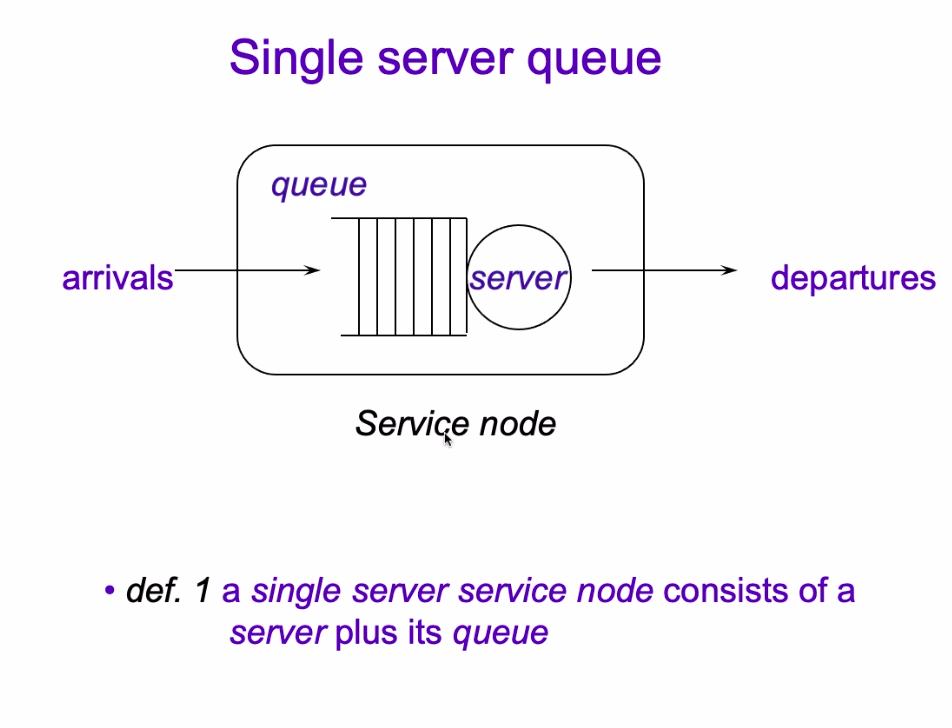
\includegraphics[scale=0.2]{images/PMCSN-1.png}\\
Ho due parti:
\begin{itemize}
\item server: la risorsa che deve essere assegnata, è singolo perché in questo modello semplice si assume che è possibile servire una singola richiesta
\item queue: mantiene tutte le altre richieste che possono arrivare per il servizio. Quando termina il servizio, viene scelta la prima richiesta in coda
\end{itemize}
Spesso si assume che le richieste per il servizio arrivino ad istanti random: non c'è correlazione tra gli istanti di arrivo delle richieste. Questa caratteristica modella bene la stragrande maggioranza dei processi di arrivo.\\ Inoltre, si assume che la coda di buffer sia infinita (non ho la linea nera alla fine), ma spesso si è interessati alla loss probability: dato che la coda è finita, voglio conoscere la probabilità che nel momento in cui una richiesta arriva questa venga rifiutata in quanto non può essere messa in attesa. Ad esempio, in comunicazione tale probabilità di perdita è proprio il livello di connettività offerto da una rete.\\ 
\subsection{Definizioni}
La coda è un elemento importante di questa astrazione, è l'area di buffer in cui possono attendere i job che non possono essere serviti. Bisognerà decidere la politica di scelta con cui si serve il job successivo, una volta che ha finito quello corrente.\\ Disciplina di scheduling è quell'algoritmo secondo il quale si sceglie un job dalla coda:
\begin{itemize}
\item FIFO: serve il job arrivato per prima nel sistema: se arriva un job ed il servizio non è disponibile, questo prende la prima posizione in coda. Un secondo job andrà dietro l'ultimo entrato, quindi gli istanti di partenza dal server saranno ordinati nello stesso modo con cui sono stati ordinati gli istanti di arrivo
\item LIFO: opposto della FIFO, i job vengono presi a partire dall'ultima posizione della coda
\item random
\item priority: i job non sono tutti uguali per il sistema, alcuni hanno valore maggiore di altri. Può esserci un criterio di priorità secondo il quale vengono scelti sempre (se ci sono) i job di priorità più alta
\item processor sharing: rappresentazione ideale di quello che succede in un sistema time-sharing, in cui ad ogni job è assegnato un quanto di tempo per usare la risorsa. TCP ad esempio divide la banda fra i diversi job che sono attivi in un certo istante di tempo, quindi tale disciplina prevede la condivisione della capacità elaborativa (avendone assegnata $\frac{1}{n}$, se ho n job) come se fossero tutti attivi in simultanea
\end{itemize}
Si parla di job non-preemptive se un job che ha iniziato il servizio non può essere interrotto. Se invece il servizio è preemptive, allora questo può essere interrotto per dare il servente ad un job a priorità maggiore (nel caso di algoritmo a priority). Quindi, la processor sharing, avendo questo meccanismo, entra nella classe delle discipline preemptive.\\ Altra caratteristica è quella del servizio conservativo: potrebbe avere senso, nel caso in cui ci siano conoscenza della caratteristica del flusso di job che arrivano, che nel caso in cui server divenga vuoto questo non prende un job e lo manda in esecuzione perché è a conoscenza del fatto che sta arrivando un flusso prioritario.\\ Nel caso in cui un server rimanga in attesa senza fare nulla, si parla di server non conservative. Faremo l'ipotesi di serventi conservativi.
\subsubsection{Primo esempio: quanto conta lo scheduling}
10 job, conosco i 10 istanti di arrivo dei 10 job: 15 47 71 111 123 152 166 226 310 320 e questi job richiedono delle unità di tempo di servizio: 43 36 34 30 38 40 31 29 36 30.\\ Tempo di risposta di un centro: tempo che passa da quando la richiesta arriva al centro a quando parte. Lo scheduling può avere un effetto enorme sulle prestazioni: calcolo la media dei tempi di servizi (del campione) = 34.7\\ Calcolo inoltre la varianza = 20.21 Il tempo di risposta medio è 26.70: qual'è la caratteristica che inficia molto negativamente su tale valore? La variabilità: prendo il campione di 10 tempi ed aumento la variabilità sommando e sottraendo 20: 63 16 54 10 18 60 51 9 56 10. La media rimane uguale, ma la varianza aumenta moltissimo, passando da 20.21 a 504.21\\ Se invece cambio lo scheduling, ordinando i tempi di servizio in modo che arrivino in ordine decrescente di richiesta (o crescente nel caso opposto). Cosa accade: da un punto di vista di media e varianza, non cambia nulla, ma cambia in termini di tempo di risposta. Infatti, nel caso di ordine decrescente (servo dal più piccolo al più grande), i tempi di risposta diminuiscono di molto. Se faccio il contrario, ovvero servo in ordine decrescente, allora ho il caso peggiore: tutti hanno davanti a se job che occupano per più tempo di quello che chiedono.\\ L'algoritmo di scheduling non costa nulla, ma il modo in cui si schedula può agire molto sulle prestazioni. La variabilità è sempre un indice negativo a livello di prestazioni
\subsection{Altri esempi-applicabilità della modellazione}
Ho un rete, conosco i route dei pacchetti, la loro frequenza di arrivo, il tempo di trasmissione e la lunghezza dei collegamenti. Con la teoria delle code, possiamo conoscere:
\begin{itemize}
\item valor medio del tempo speso nel router i
\item la distribuzione dei pacchetti nella coda al router i
\item tempo totale medio per poter andare dal punto A al punto B
\end{itemize}
L'approccio modellistico è anche usato come tool di progettazione: so che un server subirà un carico, dal punto di vista degli arrivi, raddoppiato. Dobbiamo fare in modo che gli utenti non si rendano conto di questo raddoppio, quindi che i tempi rimangano simili. Di quanto va aumentata la capacità operativa della CPU del server per poter mantenere lo stesso tempo di risposta medio?\\ La soluzione che viene subito in mente è prendere una CPU con velocità doppia, ma in realtà serve meno del doppio se l'obiettivo è quello di mantenere gli stessi tempi di risposta.\\ È possibile rendersene conto anche analiticamente, questo evidenzia quanto a volte l'intuizione può portare dalla parte sbagliata.\\ Se sostituissi la CPU con una di potenza doppia, il tempo di risposta sarebbe dimezzato rispetto a quello del giorno prima, quello che succede è che il sistema dal punto di vista del carico che sopporta e della capacità di elaborazione rimane identico, ma come se fosse velocizzato di un fattore 2. Quindi, questo comporta un tempo di risposta che è la metà.\\ Supponiamo ora di cambiare anche lo scheduling: da FIFO passiamo a processor sharing. Cambiano le cose? No.\\ Supponiamo di avere un modello di un sistema batch con due server (carico fisso): ho 6 job che possono andare nel server 1 o 2, che sono identici.\\ 
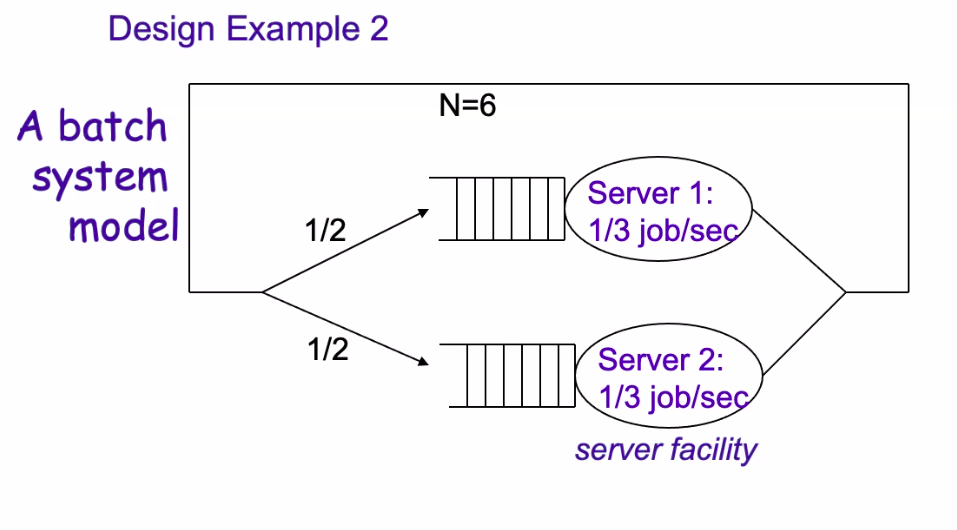
\includegraphics[scale=0.2]{images/PMCSN-2.png}\\
Supponiamo che il server 1 sia potenziato con uno che abbia il doppio della potenza, il tempo di risposta migliora? Ed il thoughput? Il miglioramento è poco e tende al nulla quanto più il numero di job del sistema cresce. Il problema è che nel sistema ho un bottleneck: posso migliorare il server quanto voglio, ma essendo il carico diviso a metà questo pesa nel calcolo della media (e noi guardiamo il calcolo della media). Se invece avessimo meno di 6 job, il miglioramento trascurabile diventa più apprezzabile? Sì, nel caso limite di uno stand alone job calcolerei la media come: 0.5$\cdot$tempo del server 1 (inverso della frequenza) + 0.5$\cdot$tempo di risposta del server 2.\\ Se invece il sistema fosse aperto (tempi di arrivo indipendenti dal completamento del servizio)? Cambia molto, migliorando uno dei due server, l'$\frac{1}{2}$ di arrivi che va nel server migliore ne risente, mentre prima c'era il bottleneck del server meno potente.\\ Altro esempio tipico, navigazione in Internet, vorrei sapere il tempo di risposta medio per una richiesta. Una situazione di questo tipo è spesso modellata, quando il numero di utenti è illimitato, infinit server; mentre se il numero è limitato sarà un centro ad un certo numero di serventi paralleli. Non ci sono code: quando arriva una richiesta c'è sempre un utente libero che aspetta la risposta.\\
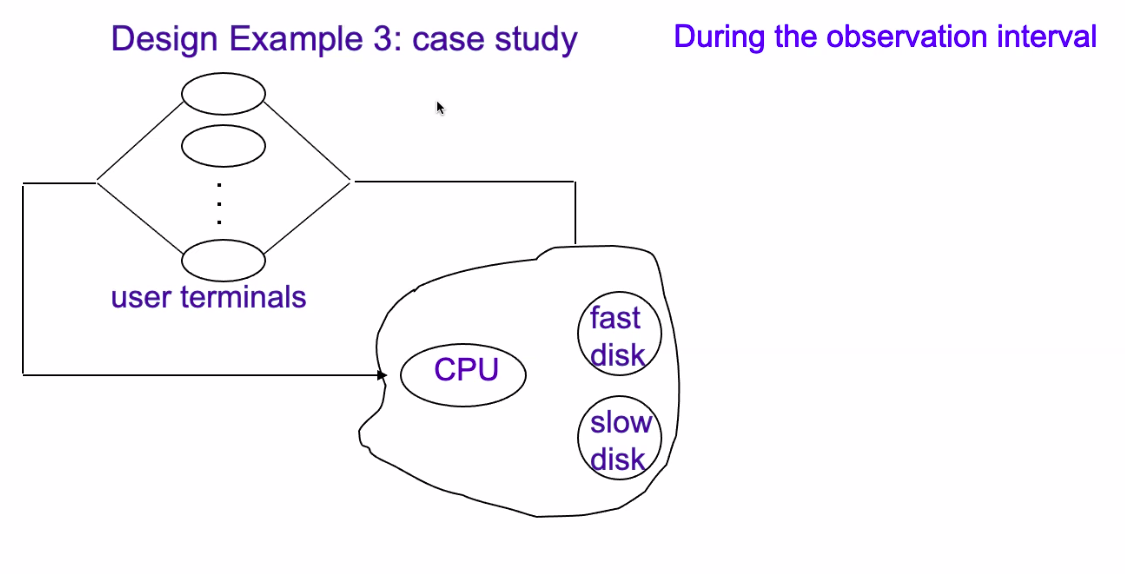
\includegraphics[scale=0.2]{images/PMCSN-3.png}\\
Osserviamo il sistema per un certo tempo (es T = 900 sec), possiamo sapere per ogni dispositivi:
\begin{itemize}
\item busy time: tempo in cui la risorsa è occupata
\item numero di completamenti, fatti nella finestra T
\item numero di completamenti del sistema
\item "think time" medio degli utenti: tempo per quanto aspettano gli utenti prima di lanciare un nuovo comando
\end{itemize}
Quale modifica è più effettiva per aumentare il throughput globale del sistema? Possiamo:
\begin{itemize}
\item prendere CPU con velocità doppia
\item fare load balancing dei due dischi
\item prendere un secondo disco veloce
\end{itemize}
Ancora una volta, la risposta è contro-intuitiva, l'approccio che è possibile usare per rispondere è l'analisi operazionale ed è "molto facile". Inoltre, è indipendente da assunzioni sulla distribuzione e non necessita di conoscere l'intera topologia della rete. Occorre però l'osservazione del sistema reale, per poter derivare le 3 quantità introdotte sopra.\\ Un altro problema molto interessante è il seguente: ho un certo budget, ad esempio in termini di potenza di calcolo ho $4\frac{job}{sec}$. Potrei avere questa potenza con 4 macchine da $1\frac{job}{sec}$ o una da $4\frac{job}{sec}$. Qui, si punta a minimizzare il tempo medio di risposta, ma occorre fare ipotesi. Partiamo dall'ipotesi che i job non siano preemtible. La soluzione migliore dipende dal carico, in particolare dalla variabilità del carico in termini di taglia del job.\\ Se c'è una alta variabilità, può accadere che un job piccolo venga bloccato da uno grande, quindi l'alternativa multi-server paralleli offre la possibilità di distribuire il carico di job piccoli in modo che non siano bloccati (ovviamente, tutti i confronti vanno fatti a parità di potenza computazionale). Viceversa, se la variabilità è bassa, conviene il singolo servente.\\ Se invece assumiamo che la classe sia preemtible, è sempre preferibile la configurazione ad un servente, perché possiamo togliere il job grande e mettere quello piccolo.\\ Il problema ha un'applicazione enorme, considerato che il server può rappresentare diverse risorse, problema è spesso il trade-off tra comprare una macchina più costosa che consuma di meno da un punto di vista energetico, oppure comprare un certo numero di macchine meno costose ma che dissipano più energia.
Un  altro problema molto diffuso riguarda il task assignment in una server farm o data center. Ho un dispatcher che si preoccupa di distribuire il workload fra diversi server. Ancora una volta, l'obiettivo del dispatcher può condizionare il tipo di politica adottata: per siti web, il dispatcher fa in modo di mantenere il carico di lavoro bilanciato fra i vari server. Nell'ambito dei super-computer la politica di bilanciamento può non essere utile.\\ Il modello è un certo numero di code ed il dispatcher davanti che deve distribuire fra le diverse code il carico che riceve. Facciamo delle assunzioni:
\begin{itemize}
\item server omogenei fra loro
\item risorsa singola per ciascun job, ogni richiesta che arriva al dispatcher userà una singola risorsa, sarebbe possibile che una richiesta possa chiedere l'uso di più di una risorsa, ma assumiamo di no.
\item scheduling delle code FIFO non-preemptible
\end{itemize}
Tra le politiche applicabili abbiamo:
\begin{itemize}
\item random: ogni job viene assegnato "lanciando una moneta equa"
\item round-robin: i job i-esimo va all'host $imodn$, dove n è il numero di host
\item shortest-queue: il dispatcher cerca di vedere il carico dell'host, manda il job all'host che ha il numero minimo di richieste
\item central-queue: unica coda, appena uno degli host diventa libero va sulla coda prende il primo job che trova
\item size-interval-task-assignment: assumiamo di conoscere la size delle richieste (in termini di carico di lavoro richiesto). I job vengono suddivisi in base alle size (si può anche avere una partizione più fine):
\begin{itemize}
\item short
\item medium
\item long
\end{itemize}
Si indirizzano i job in base alla taglia
\item least-work-left: si sceglie il server col carico minore, ogni job che arriva viene mandato al server dove a quell'istante di tempo c'è il minor carico, dove il carico è la somma delle size che si trovano in coda. Il server con valore minore sarà quello designato per ricevere il job
\end{itemize}
Le ultime due politiche sono size-based (non è sempre possibile conoscerla), mentre le altre no.\\ Supponiamo che si voglia scegliere la politica che comporta il tempo di risposta medio: dipende dalla variabilità della size:
\begin{itemize}
\item se poco variabili, la LWL comporta il tempo minimo
\item se molto variabili, la SITA comporta il tempo minimo
\end{itemize}
Quanto sarebbe quindi importante conoscere la size? In realtà, la maggior parte delle politiche usate non richiedono la conoscenza della size e si può dimostrare che in media la LWL è equivalente alla politica della central-queue: in qualche modo nella seconda politica si usa la nozione di size, in quanto il primo server che si libera all'istante di arrivo di un job è quello che aveva meno size.\\ Un'altra distinzione è fra classi di job preemptible e non: se non è preemptible non bisogna fare load balancing (non porta vantaggi) e bisogna fare altre considerazioni e studi. Il secondo è una open issue e dipende da cosa si vuole fare, se minimizzare il tempo di risposta o minimizzare il tempo di slow-down.\\ Nell'ipotesi che non vengano fatte assunzioni sulla taglia dei job e che ci siano job non-preemptive, è possibile dimostrare che finché non si mette in mezzo al taglia, è dimostrabile che non cambia nulla. Immagino ora di avere un algoritmo di scheduling FIFO preemptive, ovvero appena arriva un nuovo job ottiene subito il servizio. Per un carico che presenta almeno un minimo di variabilità si ha un miglioramento delle prestazioni enormi. Mentre invece, per un carico molto variabile, si ha un peggioramento delle prestazioni di quasi il doppio.
\section{Modelli analitici}
\subsection{Modelli a risorsa singola}
Ho una singola cosa, l'analisi guarda prevalentemente i valori medi (anche se potrei calcolare la distribuzione di probabilità)\\
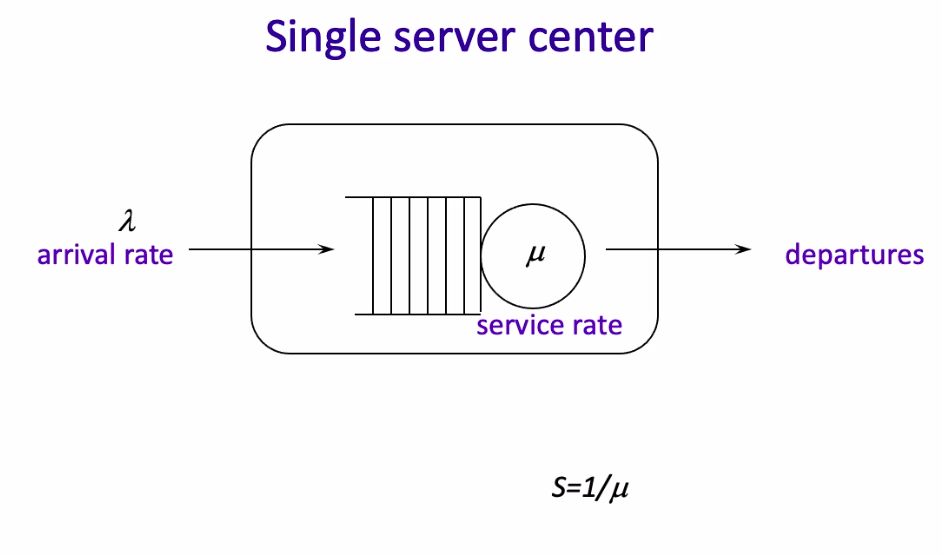
\includegraphics[scale=0.2]{images/PMCSN-4.png}\\
i parametri $\lambda$ e $\mu$ sono valori medi.\\ Si parte dalla definizione del modello concettuale (è sempre il primo passo che va fatto). Terminologia:
\begin{itemize}
\item S è il tempo di servizio ed è pari a $\frac{1}{\mu}$
\item $T_q$ è il tempo di coda
\item $T_s$ è il tempo nel sistema
\item $N_s$ è il numero nel sistema
\item $N_q$ è il numero in coda
\item U, $\rho$ è il numero nel servizio
\end{itemize}
Tipicamente, si considera il valore medio di tutte queste grandezze, un'altra misura importante, in  presenza di SLA e QoS, è P(\{$T_s > t$\}), che è la coda della distribuzione, mentre E(n)$_t$ è il numero medio di job serviti in un intervallo temporale t.\\ Quanto più $\lambda$ aumenta, tanto più cresceranno tutte le misure medie. Così come al crescere di $\mu$, che rappresenta la capacità di smaltire il traffico che arriva, le misure decresceranno.\\ Se rapportiamo E(n)$_t$ al tempo unitario 1, quindi E(n)$_1$ (possono essere secondi, minuti, ore etc...), stiamo guardando il throughput.\\ Altro fattore importante è l'utilizzazione, che ci da il rapporto tra il periodo di occupazione del servizio ed il tempo totale di osservazione.\\ Come definirlo matematicamente:\\
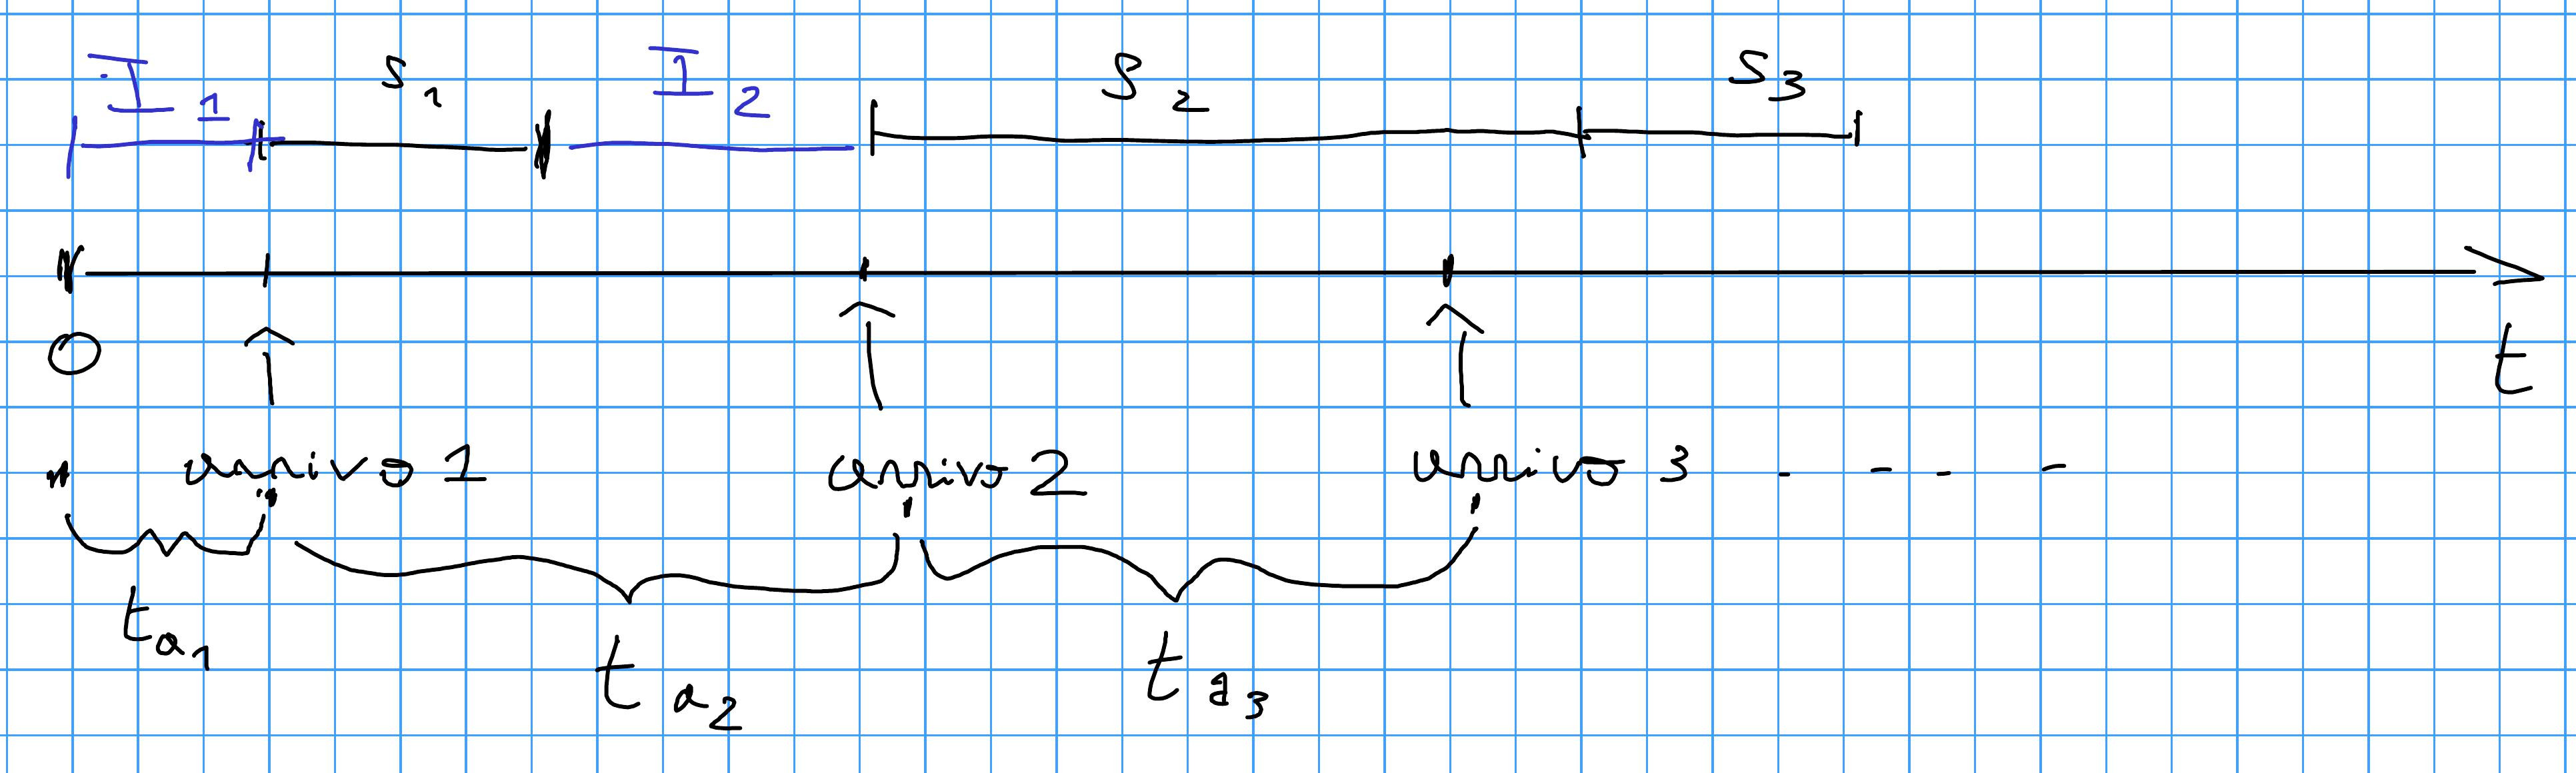
\includegraphics[scale=0.3]{images/PMCSN-5.jpeg}\\
Denotiamo con I gli intervalli in cui il servente è idle (non ha job in servizio), il tempo di occupazione totale sarà dato o da $t - \sum\limits_{i = 1}^{n} I_i$ oppure da $\sum\limits_{i = 1}^{n} s_i$.\\ Definiamo l'utilizzazione come $\rho = lim_{t-> \inf} \frac{B}{T}$.A questo punto, andiamo a sostituire i valori medi con le quantità per cui si considera il limite ottenendo $\cong \frac{E(\sum\limits_{i = 1}^{n} s_i)}{E(\sum\limits_{i=1}^{n} t_{a_i})}$.\\ Siccome gli $s_i$ sono indipendenti ed identicamente distribuite, così come le $t_{a_i}$, che sono tra l'altro esponenziali. Al di là della distribuzione, siccome hanno stessa media e stessa distribuzione, otteniamo $\frac{n\cdot E(s)}{n\cdot E(t_a)}$ = $\frac{E(s)}{E(t_a)}$ = $\frac{\lambda}{\mu}$ ed è anche $1 - P(n = 0)$, se n è il numero di job in coda. Quindi, possiamo dire che l'utilizzazione è il rapporto $\frac{frequenza\_di\_arrivo}{frequenza\_di\_servizio}$.\\ Possiamo anche dire che:
\begin{itemize}
\item $E(N_s) = E(N_q) + E(number\_in\_service)$, questo non è altro che $E(N_q) + \rho$
\end{itemize}
esempio:\\ 
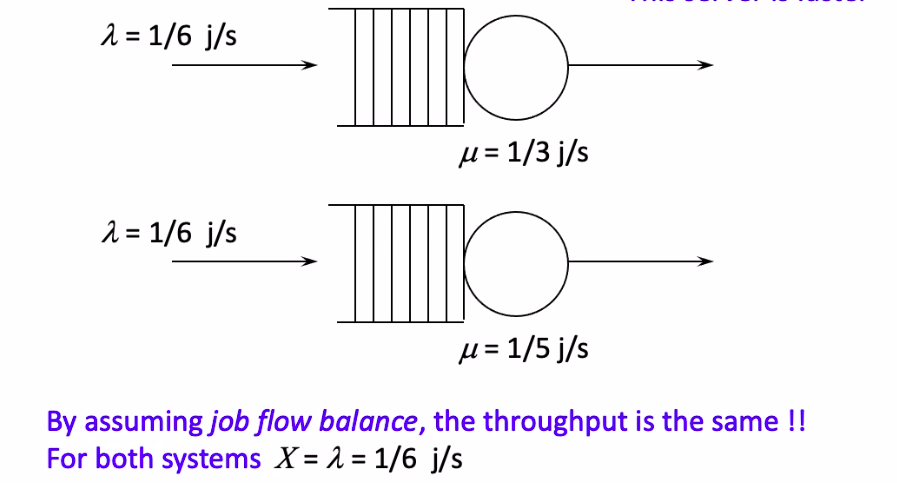
\includegraphics[scale=0.25]{images/PMCSN-6.png}
\\Il server più veloce è comunque utile, in quanto ci saranno dei tempi di risposta più brevi. Però, il minimizzare il tempo di risposta non è detto che migliori il thorughtput, come avviene in questo caso.\\ Se i centri sono in equilibrio stazionario, ovvero il flusso che entra è pari al flusso che esce (se $\lambda < \mu$ o $\rho < 1$), allora il thoughput è pari a $\lambda$. Se invece $\lambda$ è maggiore di $\mu$ allora il throughput è pari a $\mu$, ma questo vuole anche dire che la coda cresce indeterminatamente, perché il centro non riesce a smaltire le richieste in entrata.\\ Un altro modo epr definire il tempo medio di servizio, è farlo in termini di C = capacità operativa del server ($\frac{op}{s}$) e di Z = domanda media dei job (op): $E(S) = \frac{E(Z)}{C}$.
\subsubsection{Server singolo a buffer finito}
Cosa accade nel caso di buffer finito: quando la coda è piena, l'arrivo si perde (c'è tutto un altro tema quando l'arrivo alla coda piena viene mantenuta dove c'è una certa area). Qual è in questo caso il throughput? Non è più $\lambda$ e cambia anche $\rho$ in quanto non entra $\lambda$ nella coda, bensì $\lambda'$. Dove c'è un buffer finito, c'è sempre l'equilibrio perché più di tanto non entra in coda, il sistema sarà sempre in grado di servire le richieste. Per poter calcolare il throughput, avremo bisogno dei processi di Markov, calcolare la probabilità di avere lo stato vuoto e quello saturo, la probabilità di perdita sarà la probabilità di avere la coda piena.
\subsection{Server a coda multipla}
Nel caso di un centro a servente singolo, vale che:
\[
N_s =
\begin{cases}
0 \\
1
\end{cases}
\]
se $N_q = 0$. Mentre $N_s = 1 + N_q \text{se } N_q > 0$. \\ Nel caso in cui abbiamo serventi multipli vale che:
\[
N_s = 
\begin{cases}
0 \\
1 \\
. \\
. \\
m \\
\end{cases}
\]
se $N_q = 0$, mentre invece $N_s = N_q + m$ se $N_q > 0$.\\
In questo caso, cambiano tutte le misure che abbiamo effettuato:
nell'immagine, consideriamo ogni servente identico\\
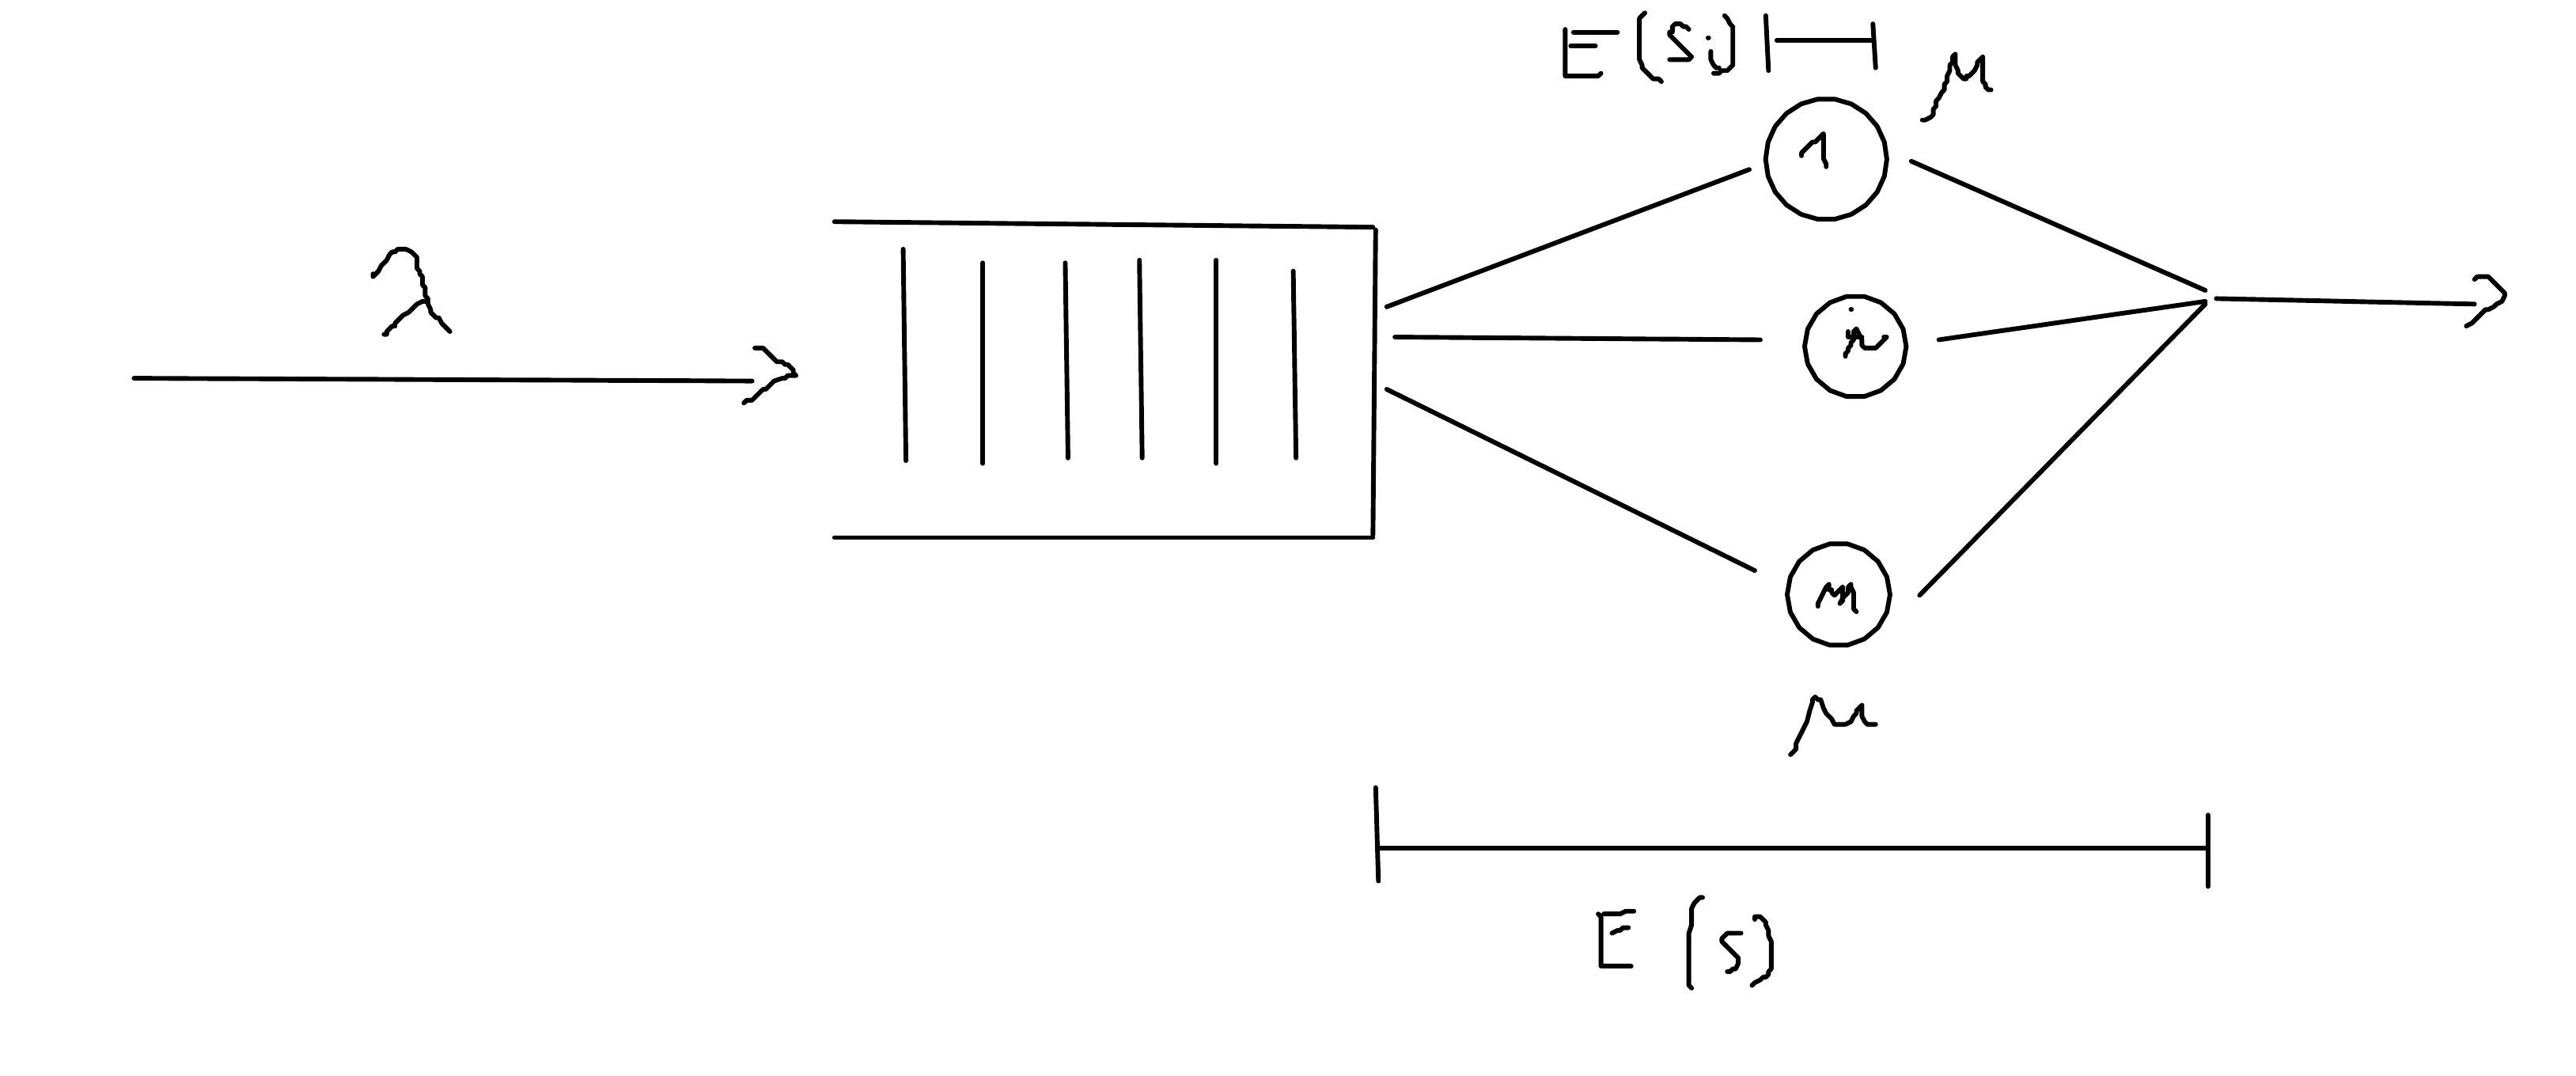
\includegraphics[scale=0.3]{images/PMCSN-903.jpeg}\\
il tempo di servizio medio, nel caso di un singolo server era $E(s)$, ora lo denotiamo con $E(s_i)$ e ci rappresenta il tempo che passa da quando un job si mette in coda a quando esce, quindi è il tempo di servizio medio su un server.\\ $E(s)$ è invece il tempo di servizio medio dall'istante in cui entra un job a quando esce un job (non per forza lo stesso), quindi è il tempo medio che occorre per liberare un server. I due tempi sono sicuramente diversi fra loro:
\begin{itemize}
\item $E(s_i) = \frac{1}{\mu}$
\item $E(s)$ è invece l'inverso del tasso globale, il multi-server ha una frequenza globale pari a $m\cdot \mu$, quindi $E(s) = \frac{1}{m\cdot \mu} = \frac{E(s_i)}{m}$
\end{itemize}
Per quando riguarda $E(N_s)$, abbiamo che:
\[
E(N_s) =
\begin{cases}
E(N_q) + \rho & \text{if } m = 1\\
E(N_q) + m\cdot \rho & \text{if } m > 1\\
\end{cases}
\]
Come viene definito $\rho$ nel caso del multi-server: in generale, sappiamo che $\rho \cong \frac{frequenza\_di\_ingresso}{max\_frequenza\_d'uscita}$, quindi andiamo a fare un prima distinzione fra:
\begin{itemize}
\item $\rho_i$, che è l'utilizzazione del singolo server
\item $\rho_{glob}$ che è l'utilizzazione globale del multi-server
\end{itemize}
Per $\rho_i$, abbiamo che il tasso d'ingresso $\lambda$ viene diviso equamente su tutti gli m centri, quindi avremo $\rho_i = \frac{\lambda}{m\cdot \mu}$; per $\rho_{glob}$, il tasso d'ingresso è $\lambda$, ma la frequenza del multi-server è pari a $m\cdot \mu$, quindi abbiamo $\rho_{glob} = \frac{\lambda}{m\cdot \mu}$. Nonostante i due fattori di utilizzazione siano uguali, cambia il significato che hanno: se ad esempio consideriamo un $\rho = 0.7$, nel caso del singolo servente, e quindi di $\rho_i$, questo corrisponde al fatto che il centro sarà utilizzato per il $70\%$, per un periodo di osservazione lungo. Per quando riguarda invece $\rho_{glob}$, avere un valore di 0.7 vuol dire che in media il $70\%$ dei server saranno pieni.\\ Per quanto riguarda le relazioni medie introdotte in precedenza, abbiamo che:
\begin{itemize}
\item $E(T_s) = E(T_q) + E(s_i)$
\item $E(T_q) = f(\lambda, \rho, E(s))$
\end{itemize}
\subsection{Legge di Little}\label{Little}
La legge di Little permette di fare delle considerazioni sui valori medi di un sistema a code (anche per l'intera rete), vale sotto determinate assunzioni:
\begin{enumerate}
\item coda con disciplina FIFO
\item capacità del servente infinita
\item flussi bilanciati
\end{enumerate}
Nonostante ciò, è possibile applicare il teorema di Little anche se non valgono alcune delle ipotesi, ad esempio se il servente non ha capacità infinita o se per un periodo di tempo di osservazione del sistema non c'è il bilanciamento dei flussi.\\
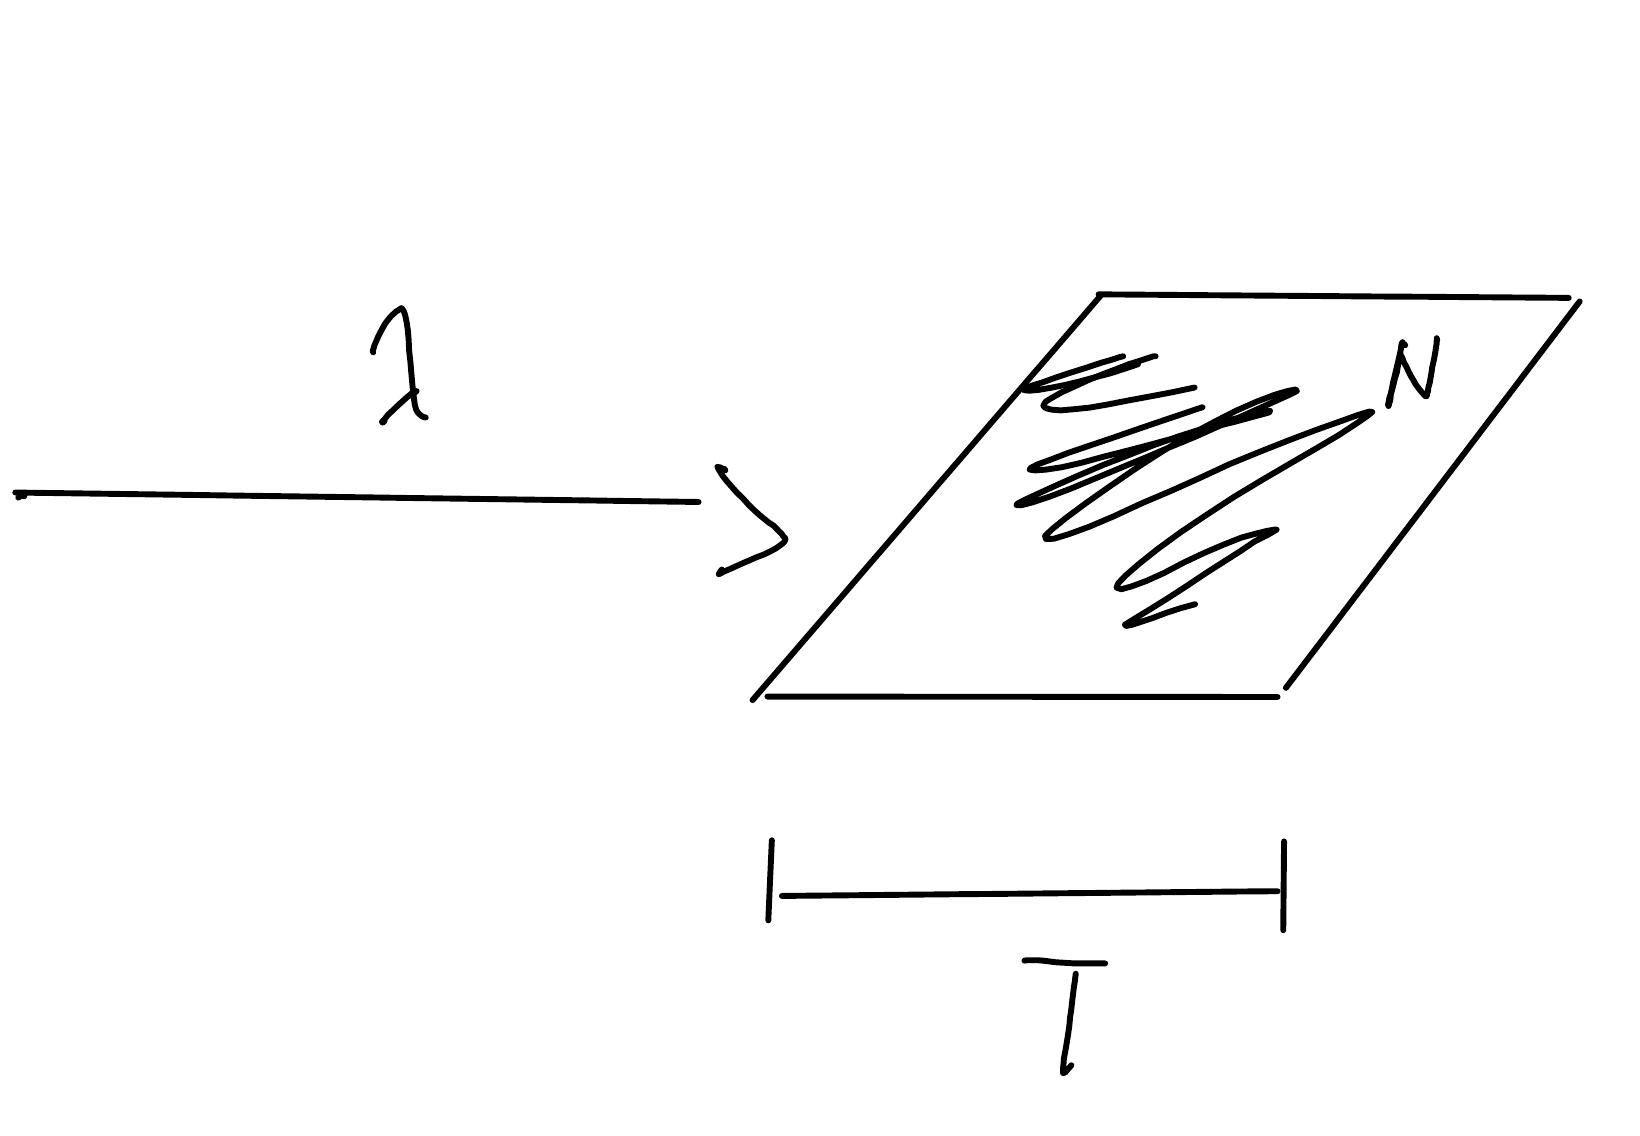
\includegraphics[scale=0.3]{images/PMCSN-903-1.jpeg}\\
\paragraph{Legge di Little:}sia $N$ il numero medio di popolazione in una "black box", $\lambda$ il tasso di arrivi medio e $T$ il tempo medio di percorrenza della box. Allora vale che $N = \lambda\cdot T$.\\ Possiamo ipotizzare che la black box sia qualunque coda:
\begin{itemize}
\item la coda + il servente: la legge ci fornisce $E(N_s) = \lambda\cdot E(T_s)$
\item la singola coda: $E(N_q) = \lambda\cdot E(T_q)$
\item il solo servente: $\rho = \lambda\cdot E(S)$
\item l'intera rete: $N = \lambda\cdot T$
\end{itemize}
È quindi possibile riscrivere tutte le relazioni trovate in precedenza per servente singolo e multi-server in funzione della legge di Little, ad esempio per il singolo centro:
\begin{enumerate}
\item $E(N_s) = \lambda\cdot E(T_s)$
\item $E(N_q) = \lambda\cdot E(T_q)$
\end{enumerate}
e vale lo stesso per il multi-server\\
\subsection{Risultati del modello analitico}
Abbiamo visto alcune relazioni per i valori medi, riscritte anche con la legge di Little. Le soluzioni note partono tutte da $E(N_q)$, cominciamo con il servente singolo.
\paragraph{Notazione di Kendall}: notazione del tipo $A/S/m/B/N/D$, dove:
\begin{itemize}
\item A si riferisce alla distribuzione degli inter-arrivi
\item S alla distribuzione del servizio
\item m al n° server
\item B alla capacità della coda
\item N alla taglia della popolazione
\item D alla disciplina della coda
\end{itemize}
Le distribuzioni più classiche sono $D, M. E_k, H_2, G$. \\ Per ora assumiamo scheduling astratto e non preemptive, quindi FIFO, LIFO non -preemptive, Random. Sembrerebbe che la FIFO, poiché rispetta l'ordine di arrivo, potrebbe essere quella che produce il tempo di risposta minimo (in quanto segue l'ordine di arrivo delle richieste), viceversa con la LIFO sembrerebbe che i job si vedano sempre bloccati da altri con tempi maggiori.\\ Ma tutte le politiche danno lo stesso \textbf{tempo di risposta medio}.\\ La notazione che utilizzeremo sarà $M/G/1$ con scheduling astratto.
\paragraph{Equazione di Khinchin Pollaczek (1930):}da una espressione per il livello di congestione nella coda, ovvero quanti job in media si trovano nella coda. $E(N_q) = \frac{\rho^2}{2\cdot (1 - \rho)} \cdot [1 + \frac{\sigma^2(S)}{E(S)^2}]$. $C^2 = \frac{\sigma^2(S)}{E(S)^2}$ vuol dire che la variabilità incide moltissimo sulle prestazioni: $C^2$ misura la dispersione dei tempi di servizio attorno alla media, quindi potrei avere distribuzioni con la stessa media, ma se la varianza è differente le cose cambiano di molto (rivedi esempi di introduzione. La congestione della coda, ovvero la popolazione media, è proporzionale a $C^2$; la formula fa riferimento ad un sistema all'equilibrio e tutti i risultati analitici fanno riferimento a sistemi all'equilibrio (o $E(N_q) -> \infty$.
\subsection{Distribuzioni a fasi}
Facciamo la distinzione fra le diverse distribuzioni a fasi,ovvero in cui si combinano più fasi esponenziali per modellare il tempo di servizio, \textbf{consideriamo sempre un solo servente, che serve un solo job}:
\begin{itemize}
\item esponenziale: il tempo di servizio che viene caratterizzato da una fase, tasso $\mu$
\item k-Erlang: il tempo di servizio che viene caratterizzato con la k-Erlang è la successione di k tempi, dove ciascuna fase è esponenziale. Le fasi sono uguali fra di loro, con tasso $\mu k$, un job che prende servizio termina tutte le k fasi e poi esce
\item distribuzione iper-esponenziale a 2 fasi: c'è una alternanza con probabilità $p$ fra due tempi esponenziali. I due tempi sono legati da una relazione, che dipende da $p$:
\begin{itemize}
\item tasso del 1° stadio è $2p\mu$
\item 2° stadio ha tasso $2(1-p)\mu$
\end{itemize}
quindi cambieranno le frequenze di servizio.\\ Quando $p = 0.5$, i due stadi sono equiprobabili, hanno entrambi tasso $\mu$, quindi l'iper-esponenziale diventa una esponenziale. Tanto più $p$ si allontana da 0.5, tanto più cresce la variabilità fra i due diversi possibili tempi
\item distribuzione di Cox: può modellare qualsiasi distribuzione. Può avere un numero arbitrario di fasi, ciascuna di esse è esponenziale ma al contrario della Erlang, dopo ciascuna fase possono accadere due cose (esclusa l'ultima fase):
\begin{itemize}
\item o si esce, questo accade nella fase i con probabilità $b_i$
\item o si passa all fase successiva e questo accade nella fase i con probabilità $a_i$
\end{itemize}
ovviamente devono valere le classiche regole, ovvero $a_i = 1 - b_i,  \forall i$ ed inoltre per lo stato finale k abbiamo $b_k =1, a_k = 0$.
\end{itemize}
Riscrivendo la KP in termini di $C^2$, otteniamo $E(N_q) = \frac{\rho^2}{2\cdot (1 - \rho)} \cdot [1 + C^2]$, dove $C^2$ dipende dalla distribuzione :
\begin{itemize}
\item D: $C^2 -> 0$
\item $E_k$: $C^2 = 1 + \frac{1}{k}, k \geq 1$
\item M: $C^2 = 1$
\item $H_2$: $C^2 = g(p) = \frac{1}{2\cdot p\cdot(1-p)} - 1$. Per $p = 0.5$, riotteniamo la $C^2$ di una M, mentre al crescere di $p$ cresce anche il termine $C^2$.
\end{itemize}
esempio: utilizziamo la KP per ricavare il tempo medio di attesa in coda. $E(T_q) = \frac{E(N_q)}{\lambda} = \frac{\rho^2}{\lambda\cdot 2\cdot(1-\rho)}\cdot(1 + C^2)$, scrivo uno dei $\rho$ al numeratore come $\lambda\cdot E(S)$ ed ottengo $\frac{\lambda\cdot E(S)\cdot \rho}{\lambda\cdot 2\cdot(1 - \rho)}\cdot (1 + C^2) = \frac{E(S)\cdot \rho}{1 - \rho}\cdot \frac{(1 + C^2)}{2}$. Anche per un fattore $\rho$ basso, ad esempio 0.5, il coefficiente $C^2$ per le heavy tails deve essere almeno pari a 25, quindi $\frac{1 + C^2}{2} = 13$, ovvero il tempo di attesa medio può diventare 13 volte il tempo di servizio.\\Nella tabella sono riportati in base al service time, $E(N_q)$ ed $E(T_q)$:\\\\
\begin{tabular}{ |c|c|c| }
\hline
Service time & $E(N_q)$ & $E(T_q)$\\
 & $\frac{p^2}{2\cdot (1 - \rho)} \cdot [1 + C^2]$ & $\frac{E(S)\cdot \rho}{1 - \rho}\cdot \frac{(1 + C^2)}{2}$\\
 &  & \\
Deterministic M/D/1 & $\frac{\rho^2}{2\cdot(1 - \rho)}$ & $\frac{\rho\cdot E(S)}{2\cdot(1 - \rho)}$\\
 &  & \\
Markovian M/M/1 & $\frac{\rho^2}{1 - \rho}$ & $\frac{\rho\cdot E(S)}{1 - \rho}$\\
 &  & \\
k-Erlang M/$E_k$/1 & $\frac{\rho^2}{2\cdot(1 - \rho)}\cdot (1 + \frac{1}{k})$ & $\frac{\rho\cdot E(S)}{2\cdot(1 - \rho)}\cdot (1 + \frac{1}{k})$\\
$\sigma^2(S) = \frac{E(S)}{k}$ &  & \\
 & & \\
Iper-esponenziale M/$H_2$/1 & $\frac{\rho^2}{2\cdot(1 - \rho)}\cdot(1 + g^2(p))$ & $\frac{\rho\cdot E(S)}{2\cdot(1 - \rho)}\cdot(1 + g(p))$\\ 
$\sigma^2(S) = E^2(S)\cdot g(p)$ &  &  \\
\hline
\end{tabular}\\\\ Al di là delle formule, è interessate notare come tutti i valori siano indipendenti da $C^2$.\\ esempio: richiamiamo l'esempio del provider che deve aumentare la potenza di calcolo per far si che gli utenti, nonostante il tasso di arrivi sia raddoppiato, sperimentino lo stesso tempo di risposta. Mostriamo in particolare come, se raddoppia la potenza il tempo di risposta risulta dimezzato:
\begin{itemize}
\item in partenza avevamo $\lambda, \mu, \rho$
\item ora, abbiamo $\lambda' = 2\cdot \lambda$, $\mu' = 2\cdot \mu$, ma $\rho' = \rho$
\end{itemize}
$E(S)'$ diviene pari ad $\frac{E(S)}{2}$, quindi ora consideriamo $E(T_s') = E(T_q') + E(S')$.Per quanto riguarda $E(T_q')$, vedendo le formule sopra, questo viene dimezzato (in quanto $E(S)$ è la metà), ed è quindi pari a $\frac{E(T_q)}{2}$. Quindi, abbiamo che $E(T_s') = \frac{E(T_q)}{2} + \frac{E(S)}{2} = \frac{E(T_s)}{2}$, quindi raddoppiando la potenza si dimezza il tempo di risposta.\\ Valgono le relazioni:
\begin{itemize}
\item $E(N_q)_D \leq E(N_q)_{E_k} \leq E(N_q)_M \leq E(N_q)_{H_2}$
\item $\sigma^2(N_q)_D \leq \sigma^2(N_q)_{E_k} \leq \sigma^2(N_q)_M \leq \sigma^2(N_q)_{H_2}$
\end{itemize}
C'è sensitività al tempo di servizio, visto che $E(N_s) + \rho$, vale lo stesso ordinamento. Con Little è possibile vedere la stessa cosa sui tempi, ma vale solo sulla media; per il momento del II ordine invece non vale.\\ Per quanto riguarda la sensitività allo scheduling, sono uguali sia media e varianza perché KP vale per ogni servizio astratto. Lo stesso vale per $E(N_s)$ ed ancora per $E(T_q)$, ma non per $\sigma^2(T_q)$ perché come abbiamo visto, lo scheduling conta.\\ Ad esempio, per uno scheduling LIFO, c'è la maggiore variabilità:\\
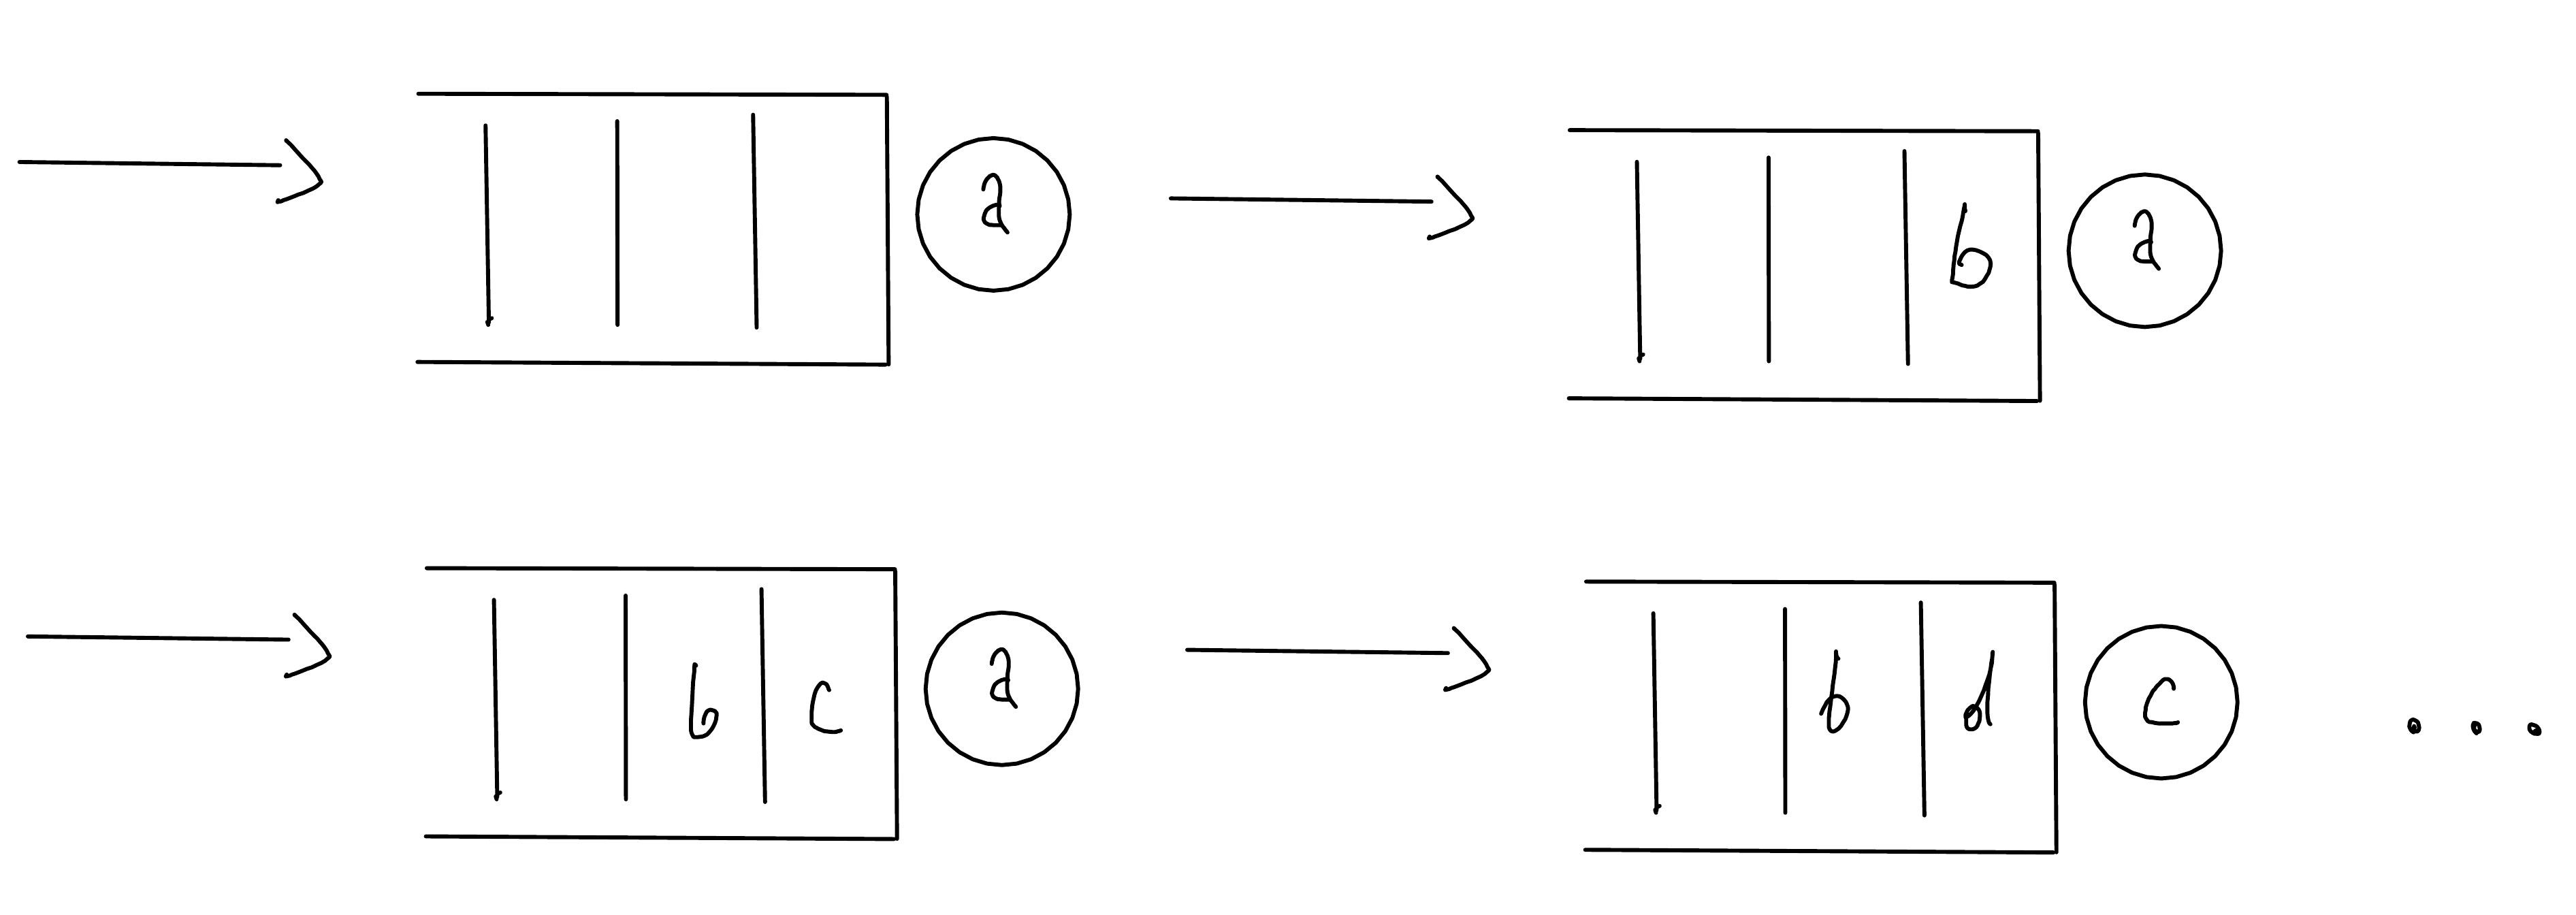
\includegraphics[scale=0.3]{images/PMCSN1003.jpeg}\\ in questo caso, b si vede arrivare sempre dei job e quindi risente del tempo di esecuzione di questi. L'esempio fa riferimento alla sola varianza, dato che nella media di tutti i possibili casi non conta, ed inoltre vale se $\rho$ è grande, in quanto questo corrisponde ad un'alta probabilità che al suo arrivo b trovi la coda piena.\\ Se consideriamo una esponenziale di parametro $\frac{1}{\mu}$:
\begin{itemize}
\item la k-Erlang ha $f_i(x) = k\mu e^{-k\mu x}$, media e varianza saranno divise per k
\item per l'iper-esponenziale, abbiamo che il singolo stadio  è una esponenziale: una sarà di param $2p \mu$ e l'altra $2(1 - p)\mu$. Per la media si fa la somma pesata delle due medie, e viene = $\frac{1}{\mu}$; per quanto riguarda la varianza abbiamo $\sigma(X) = g(p)(\frac{1}{\mu})^2$, dove $g(p) = \frac{1}{2p(1 - p)} - 1$ e tanto più ci allontaniamo da 0.5, tanto più p decresce e $g(p) -> \infty$
\item per distribuzioni generiche, abbiamo la distribuzione di Cox (può venire una distribuzione complessa). Ogni stadio è esponenziale di media $\frac{1}{\mu_i}$, dove i vari $\mu_i$ possono essere differenti e se $t_1, t_2, ..., t_k$ sono i tempi spesi in ciascuno stadio il tempo totale t è:
\begin{itemize}
\item t = $t_1$ con probabilità $b_1$
\item t = $t_1 + t_2$ con probabilità $a_1\cdot b_2$
\item t = $t_1 + t_2 + t_3$ con probabilità $a_1\cdot a_2 \cdot b_3$
\item ...
\end{itemize}
\end{itemize}
\subsubsection{Distribuzioni arbitrarie}
È sempre possibile trovare una distribuzione di Cox che approssima bene la funzione arbitraria, occorre guardare alla trasformata di Laplace e distinguere i casi in cui sia razionale o no:
\begin{itemize}
\item[a)] se è razionale, possiamo approssimare $C_k(t) = f(t)$ per un certo k, esatto o con una certa precisione nota
\item[b)] altrimenti, serve una $f(t) \approx g(t)$, in cui l'errore è noto ed a questo punto $C_k(t) \approx g(t)$, ma c'è un errore di sicuro
\end{itemize}
\subsubsection{Confronti}
Consideriamo un esempio con distribuzione esponenziale, $E(S) = 1s$, $\mu = 1 \frac{job}{s}$, se andiamo a graficare $E(T_q)$ in funzione di $\rho$ vediamo come dopo un valore di 0.7, la curva cresce velocemente a $\infty$.\\ Se confrontiamo con una k-Erlang (con k = 3), a parità di $E(S)$ (o il confronto non avrebbe senso), con $\mu = 2 \frac{job}{s}$, abbiamo come frequenza del singolo stadio $\frac{\mu}{k}$, $E(S_i) = \frac{0.5}{3} = 0.1666... s$ (tempo medio nello stato i) ed un $\sigma^2(S) = \frac{1}{k}\cdot (\frac{1}{\mu})^2 = 0.08333...$, un'esponenziale di stessa media avrebbe varianza pari a 0.25 (la varianza * 3).\\ Considerando infine una iper-esponenziale, con stessa $E(S)$, $\mu = 2 \frac{job}{s}$, $p = 0.2$ abbiamo che il primo stato ha un tasso pari a $2\cdot \rho\cdot \mu = 0.8 \frac{job}{s}$, mentre il secondo stato pari a $2\cdot(1 - \rho)\cdot \mu = 3.2 \frac{job}{s}$, quindi in media il 20\% del traffico riceve un servizio con tempo pari ad $\frac{1}{3.2}$, molto più basso di quello ricevuto in media dal restante 80\% del traffico.\\ esercizio:\\ un sistema TP accetta e processa uno stream di transazioni, mediate tramite un buffer grande.
\begin{itemize}
\item Le transazioni arrivano in modo random (distribuzione dei tempi di inter-arrivo random)\\
\item il server TP è in grado di servire transazioni ad un certo service rate
\end{itemize}
Se il tasso di arrivi e di servizio raddoppiano, sappiamo che il tempo di risposta dimezza. Supponiamo che $\lambda = 15 tps$ ed il tempo di servizio medio per transazione sia $E(S) = 58.37ms = 0.05837 s$. Cosa succede al tempo di risposta medio se la frequenza di arrivo cresce del 10\%?\\ $\lambda' = 16.5 tps$, $\rho = 87.56\%$, ora il $\rho' = 96.31\%$. Cosa possiamo dire su $E(S)$: siccome t. medio di servizio non è cambiato possiamo ragionare sul tempo medio di attesa. $E(T_q) = \frac{\rho}{1 - \rho}\cdot (\frac{C^2 + 1}{2})\cdot E(S)$, al cambiamento di $\rho$, i due termini che non vi dipendono non cambiano, quindi valutiamo il rapporto fra $E(T_q)$ ed $E(T_q')$: $\frac{E(T_q)}{E(T_q')} = \frac{\frac{\rho}{1 - \rho}}{\frac{\rho'}{1 - \rho'}} = \frac{7.0354}{26.1039} \simeq \frac{1}{3.7}$. Tempo di attesa quasi quadruplicato.
\subsection{Proprietà di mancanza di memoria e distribuzioni di probabilità}
La classe delle distribuzioni a fasi è molto importante, perché permette di modellare una distribuzione generale. La distribuzione esponenziale gode della memoryless property: informalmente, la RV non si ricorda del passato e si comporta come se fosse una variabile nuova, quindi il comportamento dipende solo dal presente.\\ esempi: supponiamo che la rv X sia il tempo trascorso in un negozio in un certo giorno della settimana dall'istante di apertura all'istante in cui entra il primo cliente. Oppure X sia il tempo da quando un server viene acceso a quando arriva la prima richiesta al server. La proprietà di mancanza di memoria fa un confronto fra la distribuzione di probabilità che valuta il fenomeno dall'istante 0 e la distribuzione che valuta il fenomeno aleatorio prima del momento in cui avviene per la prima volta un evento. Le due distribuzioni sono identiche.\\ Le uniche distribuzioni che soddisfano questa proprietà sono l'esponenziale e la geometrica; questa proprietà semplifica moltissimo l'analisi.\\ esempio: due utenti in fila alla posta, arriva un terzo utente. Qual è la probabilità che A sia l'ultimo ad uscire? $\frac{1}{2}$, uno fra B e C se ne andrà, quindi poi uscirà uno fra A ed il rimanente. Siccome i tempi di servizio sono esponenziali, la probabilità che finisca A o il rimanente è il $50\%$, non c'è influenza della storia passata.\\ Supponiamo di avere una v.a esponenziale di parametro $\frac{1}{\mu}$, quale è $P(X \leq t)$? = $1 - e^{-\mu t}$. Se condiziono invece rispetto al fatto che la v.a non ha terminato a $t_0$ e voglio scoprire la probabilità che termini a $t + t_0$, $X - t_0$ è \textbf{tempo di servizio rimanente}.\\ $P(X \leq t_0 + t | X > t_0) = \frac{P(X \leq t_0 + t \cap X > t_0)}{X > t_0} = \frac{P(X \leq t_0 + t) - P(X > t_0)}{P(X > t_0)} = ... = 1- e^{-\mu t}$
\subsubsection{Costante di decadimento dell'esponenziale}
L'esponenziale ha un'altra proprietà particolare: $f(t) = \lambda e^{-\lambda t}$, la calcolo in alcuni punti:
\begin{itemize}
\item $f(0) = \lambda$
\item $f(1) = \lambda e^{-\lambda} = f(0)e^{-\lambda}$
\item $f(2) = \lambda e^{-2\lambda} = f(1)e^{-\lambda}$
\item ...
\item $f(n) = f(n-1)e^{-\lambda}$
\end{itemize}
La media è $\frac{1}{\lambda}$, ed $f(\frac{1}{\lambda}) = \lambda e^{-1}$ ovvero: l'esponenziale parte da un punto che è il suo parametro e crolla, valutando f nella media $\frac{1}{\lambda}$ scopro che il suo valore iniziale è stato ridotto dell'$e^{-1}\%$, quindi la media è il tempo per ridurre la quantità iniziale del $1 - e^{-1} \%$. Questa viene detta costante di tempo ($\frac{1}{\lambda}$): se valuto la funzione di distribuzione nella media $\frac{1}{\lambda}: F(\frac{1}{\lambda}) = \int_{0}^{\frac{1}{\lambda}} f(t) dt = 1 - e^{-1} = 0.6321$.\\
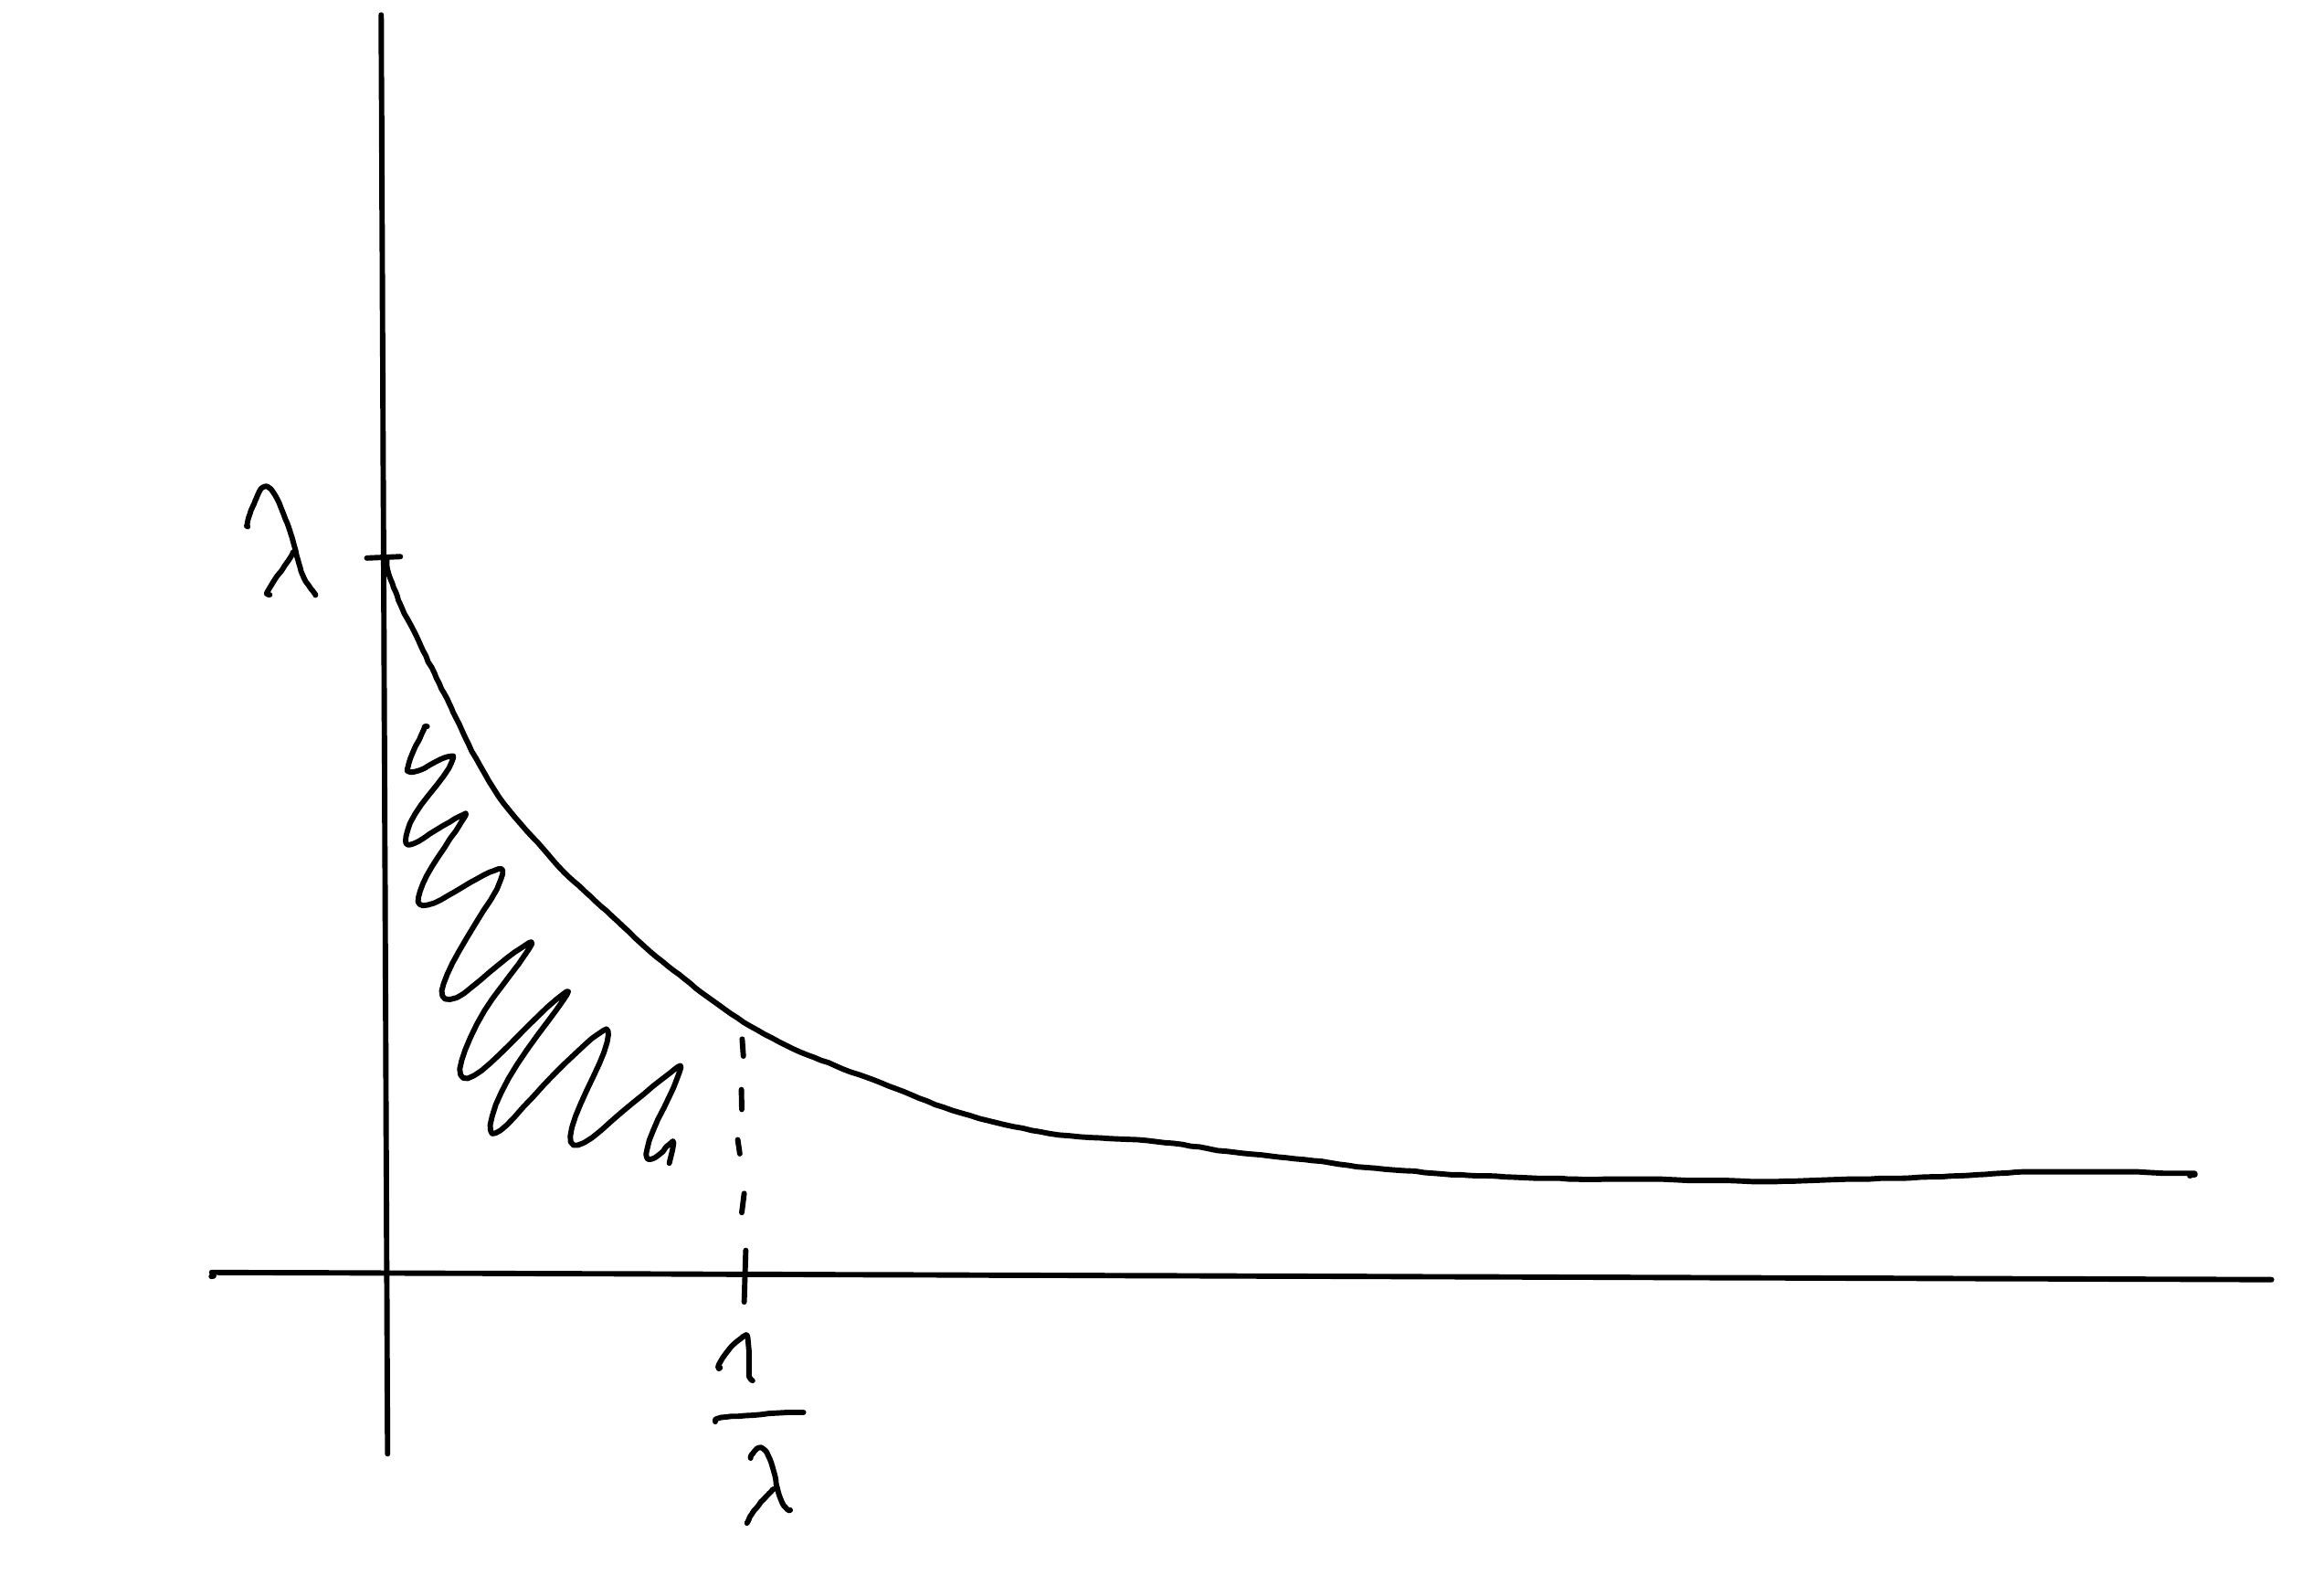
\includegraphics[scale=0.3]{images/PMCSN-exp.jpeg}\\
È indipendente da $\lambda$: qualunque sia la costante di tempo, questo equivale al tempo necessario affinché il valore iniziale si riduca di circa il $63 \%$.
\subsection{Memoryless come tempo di vita}
Una v.a X è detta memoryless se $P(X > s + t| X > s) = P(X > t), \forall s,t > 0$, ovvero il fatto che sia passato già un tempo s non conta nulla. esempio: sia X il tempo di vita di una lampadina. La memoryless direbbe che la probabilità che la lampadina duri ancora t secondi prima che si fulmini, dato che aveva funzionato per s secondi, è la stessa che la lampadina funzioni per almeno t.\\ Vediamo in termini di distribuzioni, non considerando la memoryless: considero tutte le distribuzioni per cui questo tempo di vita trascorso conta. Le distribuzioni per cui $P(X > s + t |X > s)$ decresce al crescere di s vengono dette a \textit{failure rate crescente}. Mentre, quelle per cui vale il contrario (ovvero al crescere di s la probabilità decresce), vengono dette a \textit{decreasing failure rate}.\\ esempi: il tempo di vita di una automobile è caratterizzato da un tempo di vita a increasing failure rate, nel caso chi ci riguarda di più:
\begin{itemize}
\item i tempi di vita dei job UNIX sono caratterizzati da distribuzioni decreasing failure rate: tanta più CPU ha usato un job, quanto più è probabile che ne debba usare altra
\item stesso vale per i chip: (test spesso eseguito per i chip) se non falliscono per un certo tempo, la probabilità di difetto è bassa (solitamente compaiono in un primo tempo).
\end{itemize}
\paragraph{Hazard rate function:}supponiamo di avere una v.a X continua con densità di probabilità $f(t)$ e funzione di distribuzione $F(t) = P{X < t}$, chiamiamo $r(t) = \frac{f(t)}{\bar{F}(t)}$, dove $\bar{F}(t)$ è il complementare della $F(t)$, consideriamo la probabilità che un oggetto di $t$ anni fallirà nei prossimi $dt$ secondi = $P(X \in (t, t + dt)|X > t) \approx \frac{f(t)dt}{\bar{F}(t)} = r(t)dt$, quindi la hazard rate function ci da il failure rate istantaneo.\\ Quando $r(t)$ è costante, allora la distribuzione è esponenziale.
\subsubsection{Importanza del tempo di vita rimamente}
Consideriamo un load balacing per la CPU in una rete di workstations: può essere utile migrare un job sulla workstation meno carica, per migliorare i tempi medi di risposta. Ma questo ha un costo, bisogna portarsi dietro lo stato del processo, ci sono due tipi di migrazioni:
\begin{itemize}
\item non-preemptive migration: re-alloca solo processi "nuovi", non ancora attivi
\item preemptive migration (active process migration): possibile migrare anche processi attivi
\end{itemize}
Ci poniamo delle domande: può essere utile la migrazione P, o basta la NP? E se scegliamo di usare la P, quale è una buona politica di migrazione (quale processo è meglio scegliere)?\\ Richiamiamo ancora una volta il lifetime, ricordiamo la terminologia:
\begin{itemize}
\item taglia di un job: domanda totale di CPU
\item vita di un job: utilizzo di CPU fino ad ora
\item tempo di vita di un job: richiesta totale di CPU di un job, dipende sia dalla capacità operativa che da quanto richiede (coincide sostanzialmente con la size
\item tempo di vita rimanente di un job: si riferisce ad un certo istante di tempo, la rimanente richiesta di CPU
\end{itemize}
Non per tutte le applicazioni è possibile conoscere tutti i termini, ma è sempre possibile su un sistema misurare quanta elaborazione è stata fatta, quindi è sempre possibile conoscere l'age (vita di un job).\\ 
\subsection{Distribuzioni di Pareto}\label{pareto}
(vedi slide)
Vedo le raccolte dei tempi di vita di job Unix, sembrano distribuiti esponenzialmente ma non è così: per t=2 abbiamo una decrescenza di $\frac{1}{2}$, per t=4 $\frac{1}{4}$ etc..., classe delle distribuzioni di Pareto: $f(x) = \alpha \cdot k^{\alpha} \cdot x^{-\alpha-1}$ con $k \leq x < \infty, 0 \leq \alpha \leq 2$, con code la cui misura è data da $\alpha$:
\begin{itemize}
\item $\alpha -> 0$, più variabilità e più pesantezza della coda
\item $\alpha -> 2$, il contrario
\end{itemize}
problema: hanno momento finito di ordine i sono se $\alpha > i$, quindi non possiamo valutarne la varianza.\\ Proprietà:
\begin{itemize}
\item sono a decreasing failure rate: più CPU viene usata, più continua ad usarne
\item hanno varianza infinita, la heavy tail property ci dice che una una minuscola frazione dei job molto grandi contribuisce alla metà del carico del sistema. Per esempio, con $\alpha = 1.1$, se migro i job grandi, tolgo la metà del carico dal sistema.
\end{itemize}
\subsubsection{Bounded Pareto}
L'infinito che limita la x si può togliere, si può facilmente trovare un limite finito molto grande alla size, si può passare alla classe bounded Pareto: $f(x) = \alpha \cdot x^{-\alpha - 1} \cdot \frac{k^{\alpha}}{1 - (\frac{k}{p})^{\alpha}}$ con $k \leq x \leq p, 0 < \alpha < 2$, tutti i momenti sono finiti.\\ $C^2 = 25$ è il minimo coefficiente di variazione misurato per distribuzioni di questo tipo, solitamente varia tra 25 e 49, quindi le prestazioni possono degradare moltissimo (con la variabilità), nel caso di distribuzione di questa classe.\\ Quindi, rispondendo alle due domande precedenti, la caratteristica del decreasing failure rate (quindi tutti i casi in cui l'applicazione viene ben modellata da questa caratteristica) ci porta a pensare che la migrazione è utile e può essere più sensato migrare i job vecchi. Sebbene i job vecchi potrebbe aver maturato uno stato più significativo di un job "giovane" (appena nato"), quel costo di migrazione verrà ammortizzato dal tempo in cui quel job continuerà a chiedere risorse di computazione.
\subsubsection{Pareto study}
Consideriamo una distribuzione di Pareto: $f(x) = \alpha \cdot k^{\alpha} \cdot x^{-\alpha-1}$ con $k \leq x < \infty, 0 \leq \alpha \leq 2$, $E[X] = \frac{\alpha k}{\alpha - 1}, \alpha > 1$, combinando media e varianza si ottiene il tempo di attesa $E(T_Q)$. Dalla media posso ricavare k a seconda dell'$\alpha$ che vogliamo: man mano che ci si allontana da $\alpha = 2$ ci si allontana dal caso peggiore (vogliamo $\alpha < 2$ per una heavy tail). Tutti i casi sono peggiori dell'iper-esponenziale, che è il caso peggiore di tutte le distribuzioni viste, andando verso le heavy tail e con fattori di utilizzazione alti il tempo di attesa passa dal 7 dell'iper-esponenziale a 144 per la Pareto; la variabilità ha quindi un impatto pesante.
\subsection{Risultati analitici ulteriori della KP}
Vediamo la KP nell'ottica del tempo di servizio rimanente. Ad un certo istante di tempo, la situazione di un server può essere la seguente:\\
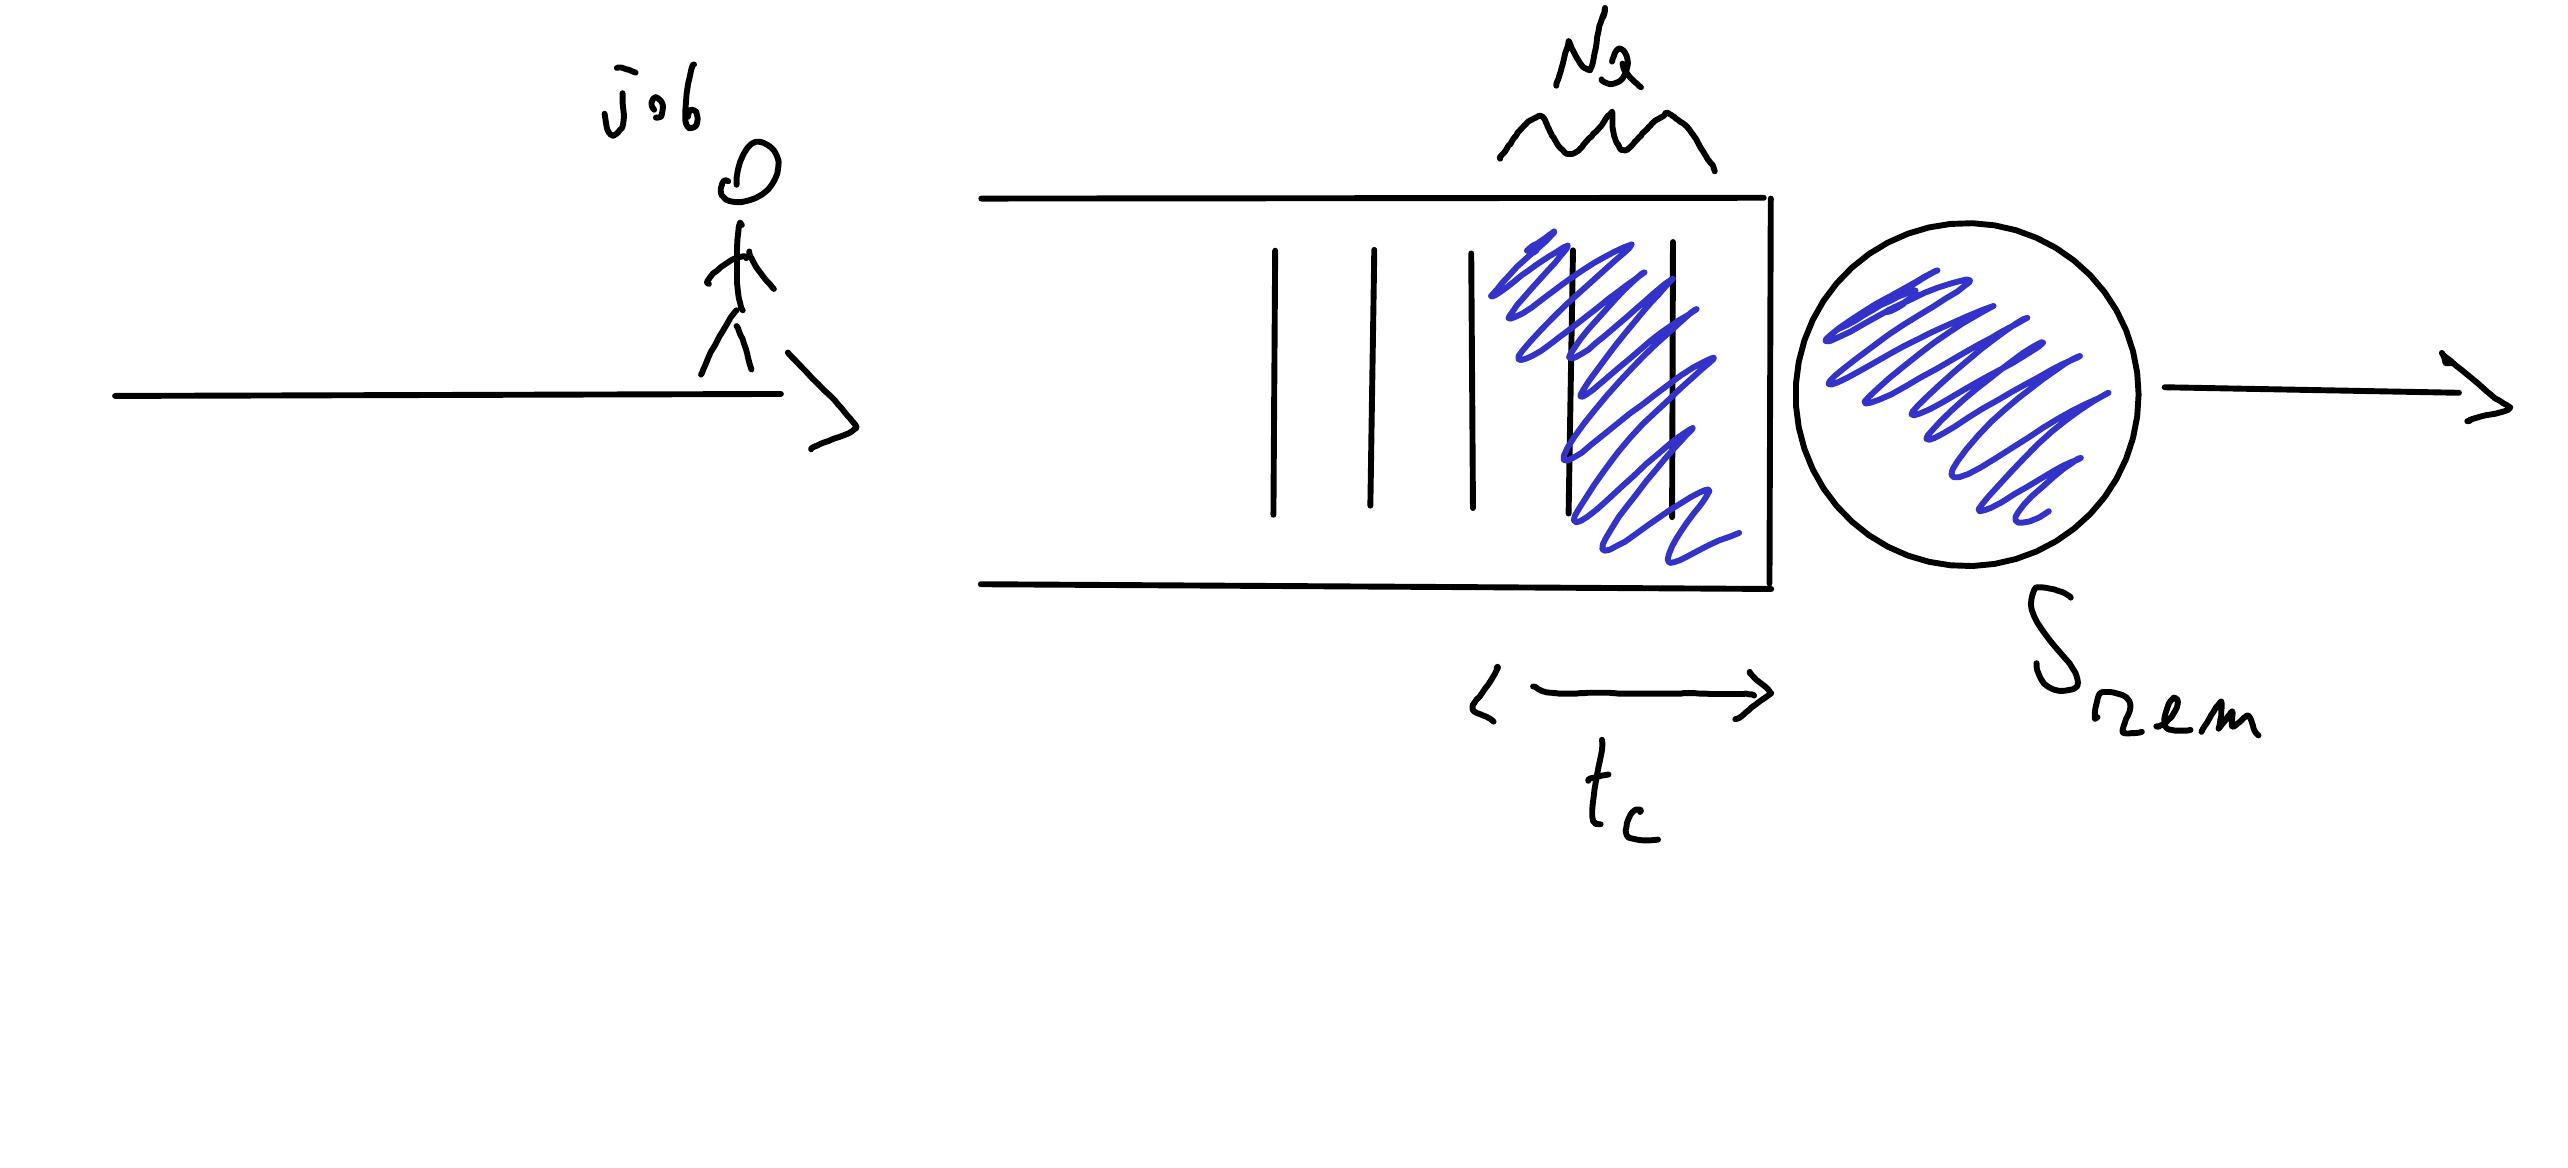
\includegraphics[scale=0.4]{images/PMCSN-1603.jpeg}\\
supponiamo che lo scheduling sia FIFO, il job che arriva dovrà attendere il tempo necessario ad elaborare i job nella coda ed il tempo di servizio rimanente del job in servizio. Il tempo di attesa sarà quindi una qualche combinazione $T_Q = t_c \oplus S_{rem}$, si può dimostrare che per \textbf{qualunque distribuzione} $E(S_{rem} = \frac{\lambda}{2}\cdot E(S^2)$. Nel caso dell'esponenziale, poiché $E(S^2) = 2\cdot E(S)^2 \rightarrow E(S_{rem}) = \frac{\lambda}{2}2E(S)^2 = E(S_{rem} = \rho E(S))$, quindi $E(T_Q) = \frac{\rho E(S)}{1 - \rho} = \frac{E(S_{rem})}{1 - \rho}$, quindi l'operazione per l'esponenziale è un prodotto di $E(S)$ con $\frac{1}{1 - \rho}$ (che non è il tempo per completare, \textbf{ma è un numero puro}).\\ Nel caso generale (KP): $E(T_Q) = \frac{\rho}{1 - \rho} \cdot \frac{C^2 + 1}{2}\cdot E(S) = \frac{1}{1 - \rho} [\frac{\sigma(S)^2}{E(S)^2} + 1]$ = $\frac{\rho}{2(1 - \rho)}\cdot[\frac{E(S^2) - E(S)^2}{E(S)^2} + 1] = \frac{\lambda E(S)}{2(1 - \rho)}[\frac{E(S^2)}{E(S)^2} - 1 + 1]$ = $\frac{\lambda}{2(1 - \rho)}[\frac{E(S^2)}{E(S)^2}]E(S)^2 = \frac{\lambda}{2}\cdot \frac{E(S^2)}{1 - \rho}$.\\ Il termine $\frac{1}{1 - \rho}$ rappresenta il fattore legato al $t_c$ (NON È UN TEMPO), siccome i due termini sono combinati con un prodotto:
\begin{itemize}
\item se uno è 0, il risultato è 0. Se $E(S_{rem}) = 0$, allora non c'è coda. Il job che arriva non deve attendere e viene subito servito
\item se uno è 1, abbiamo un invariante per il prodotto. Se il coefficiente $\frac{1}{1 - \rho}$ fosse 1, il job che arriva trova solo il job in servizio, quindi in pratica è come se non attendesse nulla
\end{itemize}
\paragraph{Tempo di risposta} per il tempo di risposta $E(T_S)$ abbiamo:
\begin{itemize}
\item M/G/1: $E(T_S) = E(T_Q) + E(S) = \frac{\frac{\lambda}{2} \cdot E(S^2)}{1 - \rho}$
\item M/M/1: $E(T_S) = \frac{\rho E(S)}{1 - \rho} + E(S) = \frac{E(S)}{1 - \rho}$.
\end{itemize}
\subsection{Scheduling astratto non-preemptive}
Riprendiamo le definizioni sullo scheduling, abbiamo dei risultati molto più forti di quelli della KP. Ricordiamo che: 
\paragraph{Definizione 1:}una politica prevede preemptive se un job può essere fermato durante la sua esecuzione e ripreso più tardi, dal punto in cui era stato fermato. Una politica è invece non preemptive se i job non possono mai essere fermati mentre sono in servizio.
\paragraph{Definizione 2:}lo scheduling si dice work conserving quando il server non è mai fermo nel caso in cui ci sia qualcuno nella coda. Può avere senso, per un server, attendere un job di taglia piccola (se sa che questo arriverà a breve), quindi il work non-conserving ha un senso.\\ C'è un risultato molto più forte della KP:
\paragraph{Teorema di Conway, Maxwell, Miller:} tutto lo scheduling astratto non preemptive mostra avere la stessa distribuzione del numero di job nel sistema: vale per $E(N_S), E(N_Q)$, quindi con Little anche per $E(T_Q)$ ed $E(T_S)$; quindi, vale per i momenti di ogni ordine (per i tempi invece, vale solo per le medie).\\ In generale $E(T_Q) = \frac{\frac{\lambda}{2} E(S^2)}{1 - \rho}$, può essere alto quando il quadrato è alto.\\ Cosa non ci piace: l'attesa in coda non ha nessuna relazione con la size del job, Mentre un job grande la tollera, in quanto l'attesa è proporzionale a quanto lui richiede, ma per job piccoli questo è poco fair. Ciò che vorremmo vedere è un tempo di risposta proporzionale alla size: chi chiede molto attende molto, chi poco attende poco.
\subsubsection{Tempo di slowdown}
Consideriamo il tempo di risposta medio per un job di taglia x: $E(T_S(x)) = E(x + T_Q(x))$, ATTENZIONE: si mette la taglia del job (x), non il tempo di servizio medio $E(S)$, perché dopo aver atteso in coda non vogliono vedere il tempo $E(S)$, bensì x. Quindi, siccome x non è una media, ma una size, inoltre $E(T_Q)$ è indipendente dalla size x, quindi otteniamo $E(T_S(x)) = x + E(T_Q)$. Definiamo una nuova misura di prestazione chiamata \textit{slowdown} (rallentamento): non valuto solo il tempo di risposta, che una misura non fair, ma anche lo slow down per size che mi dice quanto il sistema è stato fair con i job. Lo slowdown medio per job di taglia x è il tempo medio osservato rispetto all taglia del job: $E(sd(x)) = \frac{E(T_S(x))}{x} = 1 + \frac{\frac{\lambda}{2} E(S^2)}{x \cdot (1 - \rho)}$  quindi lo slowdown diventa tanto più grande, quanto più il job è piccolo.
\subsubsection{Slowdown vs response time}
Il tempo di risposta tende ad essere rappresentativo per la performance di pochi job, i più grandi tendono ad enfatizzare la performance di quelli molto grandi, visto che contano di più in media il loro tempo di risposta tendere ad essere il più grande.\\ Il tempo di slowdown tende ad essere rappresentativo per la performance della maggior parte dei job perché domina la performance del grande numero di piccoli job; vorremmo rendere $E(T_S(x))$ piccolo per x piccoli. Come fare se non si conosce la taglia x: due ragioni storiche per cui lo scheduling delle CPU è circa processor sharing :
\begin{itemize}
\item parliamo di sistemi con molte risorse, quindi è utile avere in esecuzione molteplici job perché questi richiedono diverse risorse
\item una divisione di tempo o processor sharing, in termini di modelli, fa andare avanti job piccoli senza necessariamente conoscere la taglia. Se do un n-simo di quanti (o quanto di tempo) a ciascuno, i job piccoli finiranno subito, quelli grandi continueranno a stare lì
\end{itemize}
dovrebbe essere migliore il processor sharing rispetto alla FIFO, in termini di tempi di risposta medi,perché manda via i job piccoli velocemente, ed in termini di slowdown dovrebbe essere molto meglio, perché non rallenta i job piccoli. $P(N_S = n)^{M/G/1/PS} = \rho^n (1 - \rho) = P(N_S = n)^{M/M/1/FIFO}$, riusciamo ad avere le stesse prestazioni, anche in caso di distribuzione generale. In particolare: $E(N_S)^{M/G/1/PS} = \frac{\rho}{1 - \rho} = E(N_S)^{M/M/1/FIFO}$ ed $E(T_S)^{M/G/1/PS} = \frac{E(S)}{1 - \rho} = E(T_S)^{M/M/1/FIFO}$, quindi il processor sharing, che tra l'altro modella bene molte situazioni reali, ha degli indici di prestazioni ottimi quando la variabilità è maggiore di 1. Inoltre, è insensibile alla variabilità del tempo di servizio, perché vale per distribuzione generale (infatti la variabilità non compare nelle formule), mentre nella FIFO le prestazioni sarebbero peggiori.\\ Se guardassimo delle sequenze particolari di job, potrebbero esserci prestazioni differenti:\\
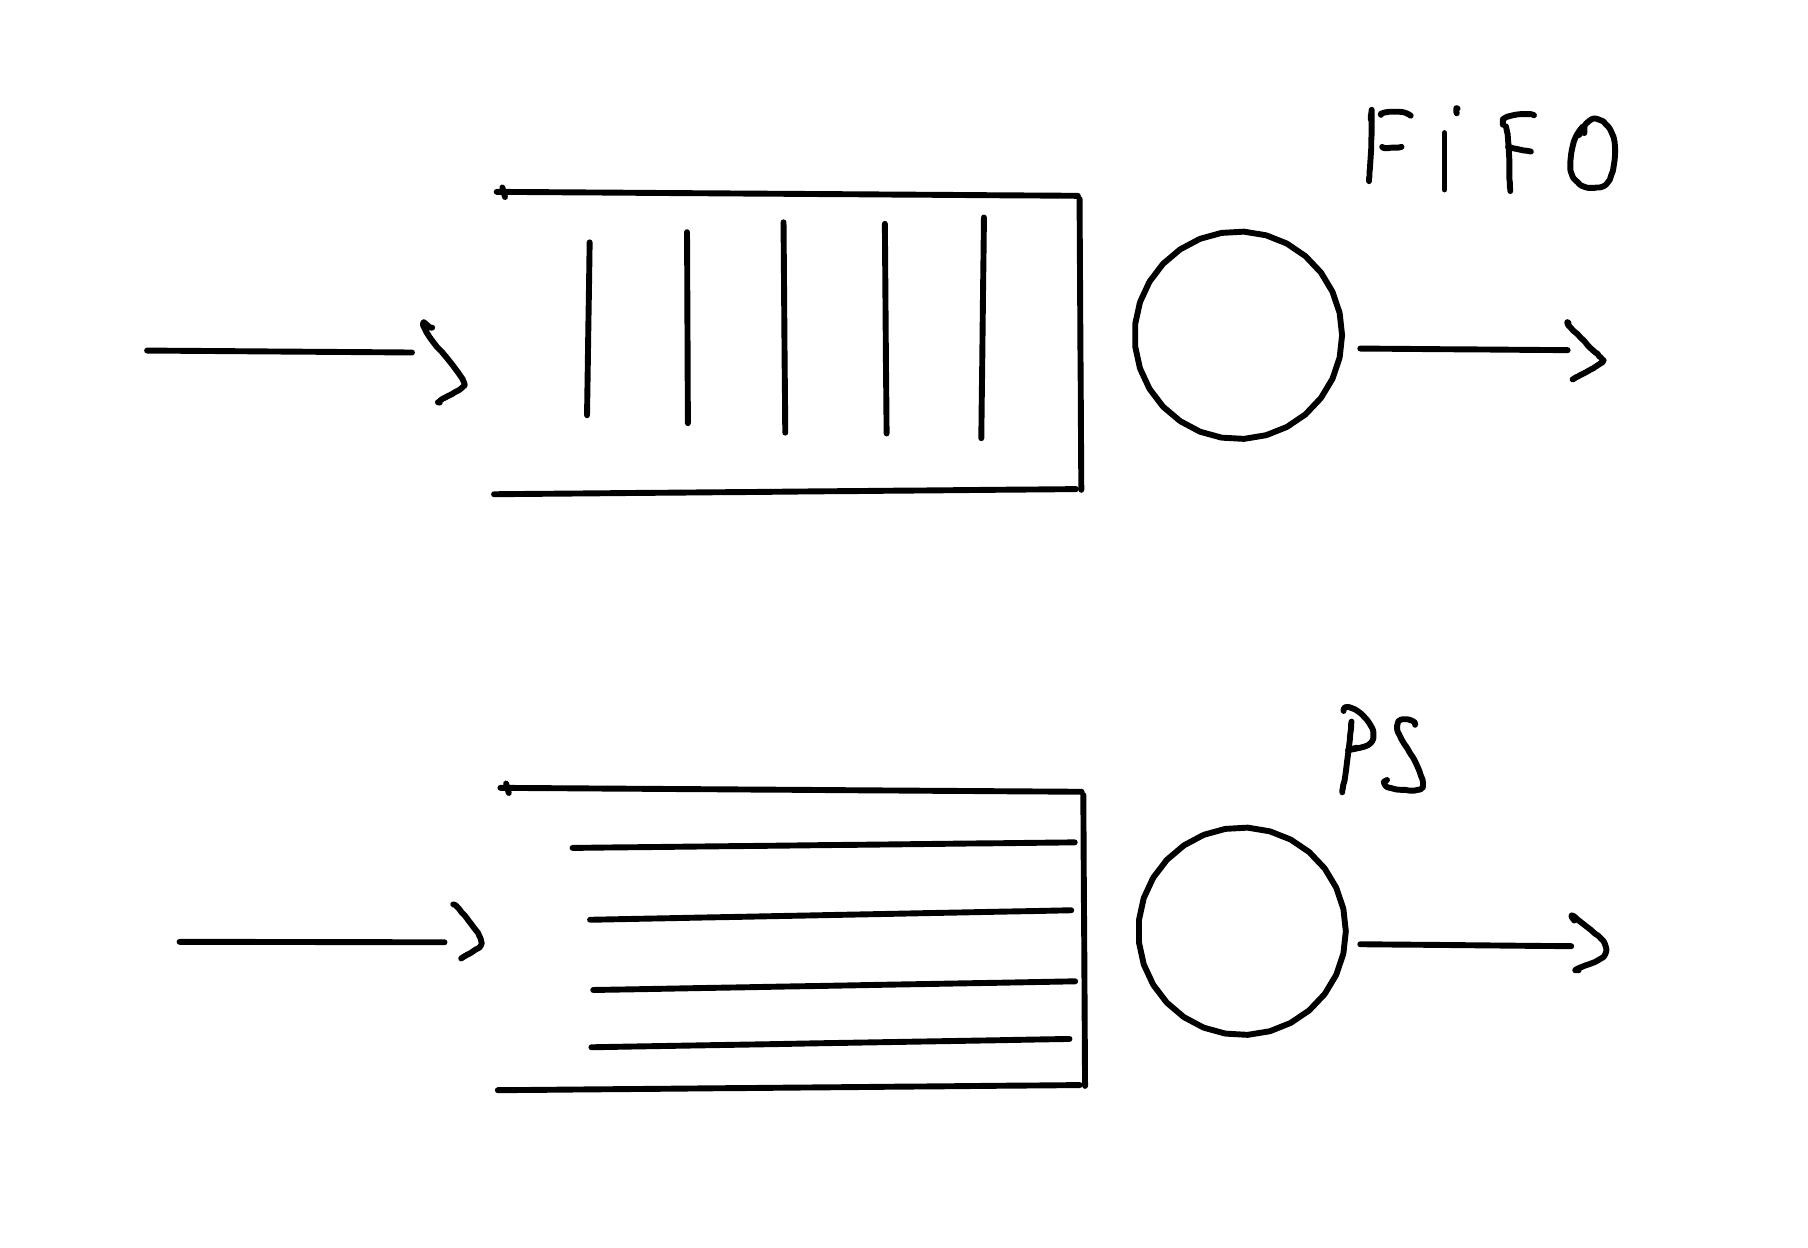
\includegraphics[scale=0.3]{images/PMCSN-1603-1.1.jpeg}\\ 
arrivano 2 job in simultanea con una taglia di 1s, per quale dei due scheduling abbiamo $E(T_S)$ più piccolo;
\begin{itemize}
\item nel caso FIFO, arrivano i due job in simultanea, il primo prende subito servizio e ci mette 1 sec. Il secondo attende 1 sec + 1 sec per il suo servizio, quindi in totale 2. In media, $1.5 s$
\item nel caso della PS, i due job dovranno stare nel centro 2 sec per poter essere entrambi serviti, quindi $E(T_S) = 2 s$, simultaneamente riceveranno la metà della capacità, nel 1° secondo $\frac{1}{2}$ della capacità a testa e nel 2° secondo l'altro $\frac{1}{2}$
\end{itemize}
quindi su alcune sequenza particolari di job la Processor Sharing può dare dei risultati peggiori.\\ In termini di slowdown abbiamo che $E(T_S(x))^{M/G/1/PS} = \frac{x}{1 - \rho}$ e quindi $E(sd(x))^{M/G/1/PS} = \frac{1}{1 - \rho}$, quindi è indipendente dalla size: tutti i job vengono rallentati dello stesso fattore, piuttosto dipende dal carico del sistema; quindi la processor sharing è lo scheduling fair per eccellenza, spesso viene usato per confronti con altri scheduling. Nel caso astratto abbiamo $E(T_S(x))^{M/G/1/abstract} = 1 + \frac{\frac{\lambda}{2}E(S^2)}{x(1 - \rho)}$. Tutti gli scheduiling preemptive non basati size hanno lo stesso tempo di slowdown $\frac{1}{1 - \rho}$. Noi vorremmo rallentare i job grandi a favore dei piccoli, ma senza conoscere la size dei job come facciamo? Sappiamo sempre di sicuro l'age dei job, ed è un indicazione della domanda rimanente: se le distribuzioni hanno decreasign failure rate, allora i job più grandi hanno con una certa probabilità una domanda rimanente più alta, quindi potremmo dare preferenza ai job con age bassa che \textbf{potrebbero essere piccoli} (per le heavy tail, consultare paragrafo 20.7).
\paragraph{Scheduling Unix}la disciplina si chiama foreground-background:\\
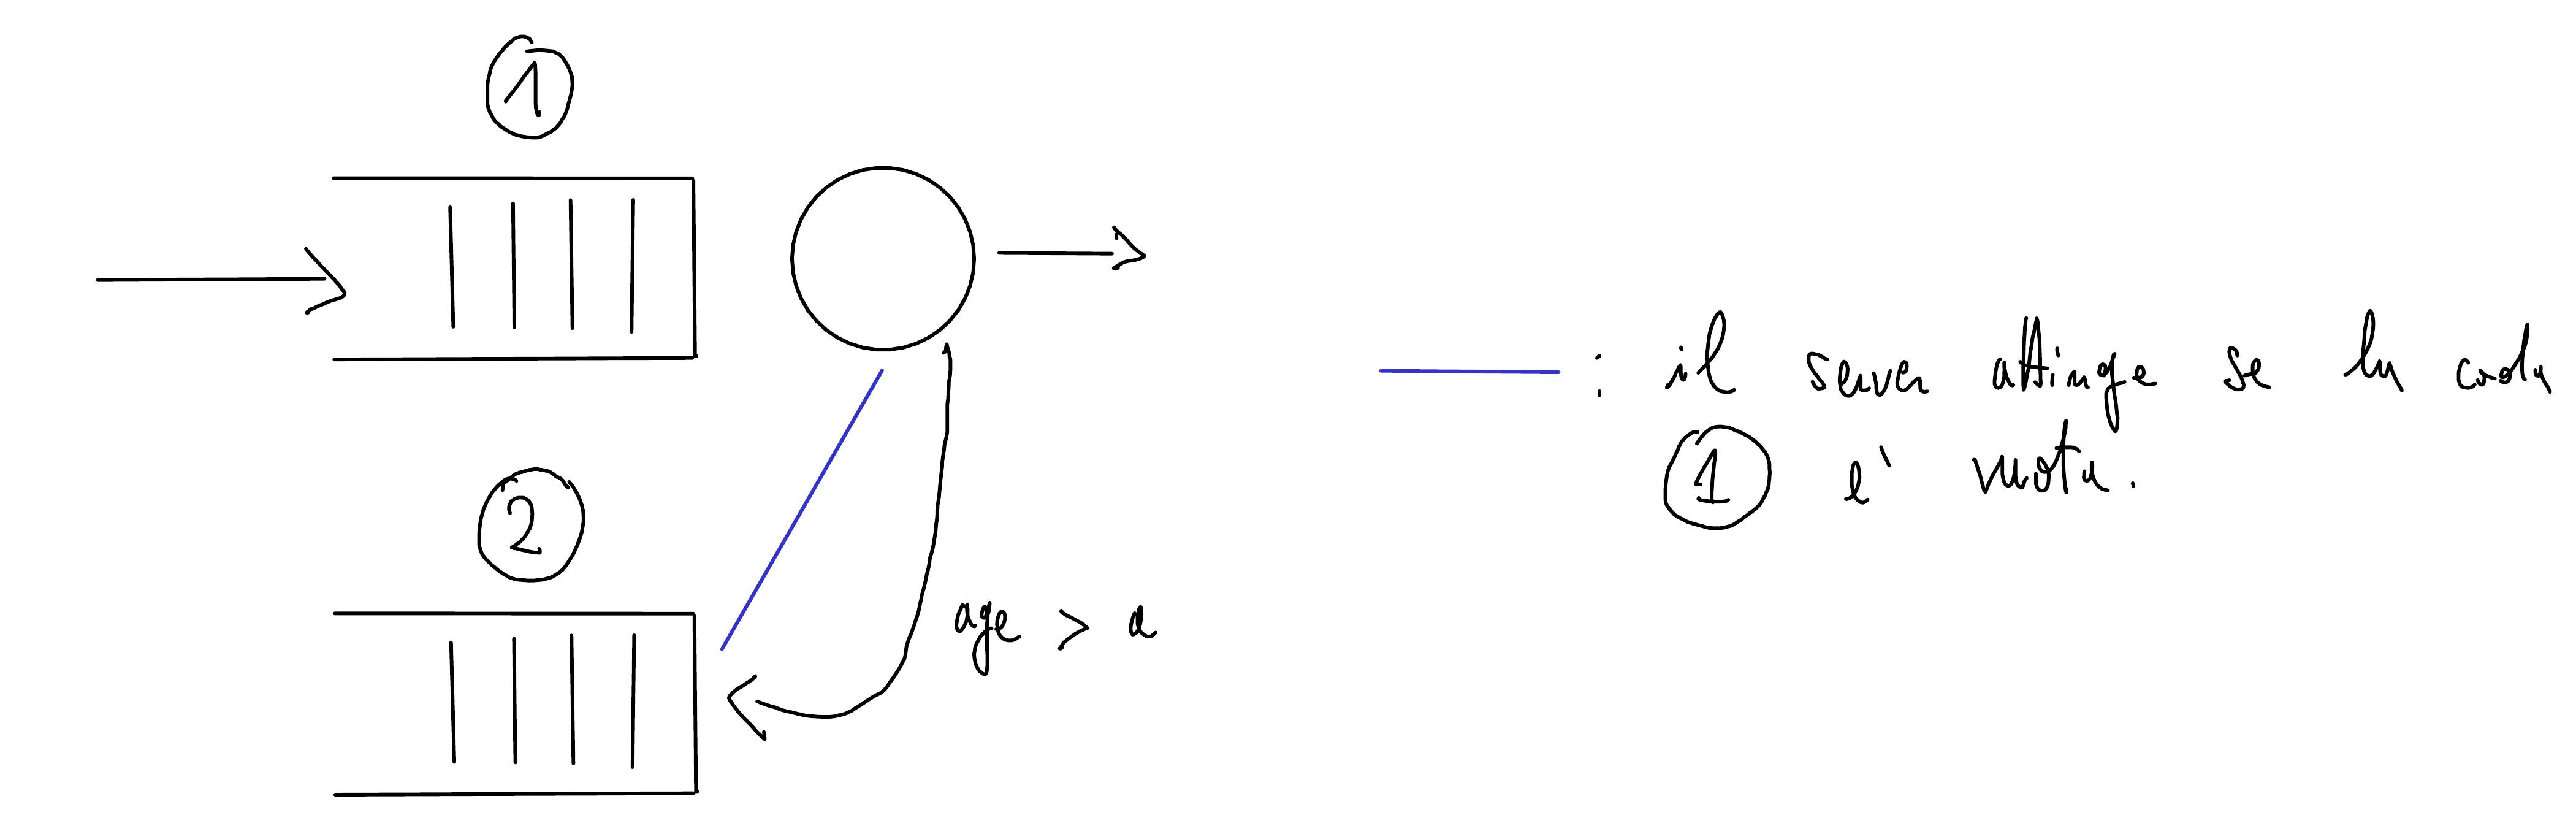
\includegraphics[scale=0.3]{images/PMCSN-1603-1.3.jpeg}\\
due code gestite in PS, tutto il traffico in I va nella prima coda che viene servita con priorità. Il server passa alla seconda coda solo quando la prima è libera, il passaggio di coda avviene mediante l'age: superato un valore a di age (parametro del sistema) di uso della risorsa, il job viene messo in coda 2. Non appena arriva qualcuno in coda 1, il server torna a servire questa coda, in modo da dare la precedenza ai job piccoli pur senza conoscerne la size, ma "giocando" sull'age.\\
Il tempo di risposta medio è abbastanza condizionato dai job con tempi di servizio alti, viceversa nel calcolo dello slowdown la metrica tiene conto di una grande parte di job piccoli. Nello slowdown, se non ci fosse attesa (perché $\rho$ è piccolo) lo slowdown sarebbe 1, la curva tende ad 1.Il tempo di risposta condizionato è invece lineare ad x. Nel caso della processo sharing, abbiamo $E(T_S(x))^{PS} = \frac{1}{1 - \rho}$: confrontando con FIFO, il tempo di risposta è sempre lineare rispetto ad x, ma lo slowdown nel caso della PS è costante e dipende solo da $\rho$.
\subsection{Utilizzazione e bilancio dei flussi}
L'utilizzazione si può vedere studiando nel tempo l'occorrere degli eventi, otteniamo $\frac{\lambda}{\mu}$. Vediamo ora il feedback
\subsubsection{Servente a coda singola con feedback}
Un job che ha completato potrebbe ancora avere necessità del server, quindi il flusso di arrivo al server è mischiato:
\begin{itemize}
\item richieste nuove
\item richieste che hanno terminato e vogliono richiedere di nuovo il servizio
\end{itemize}
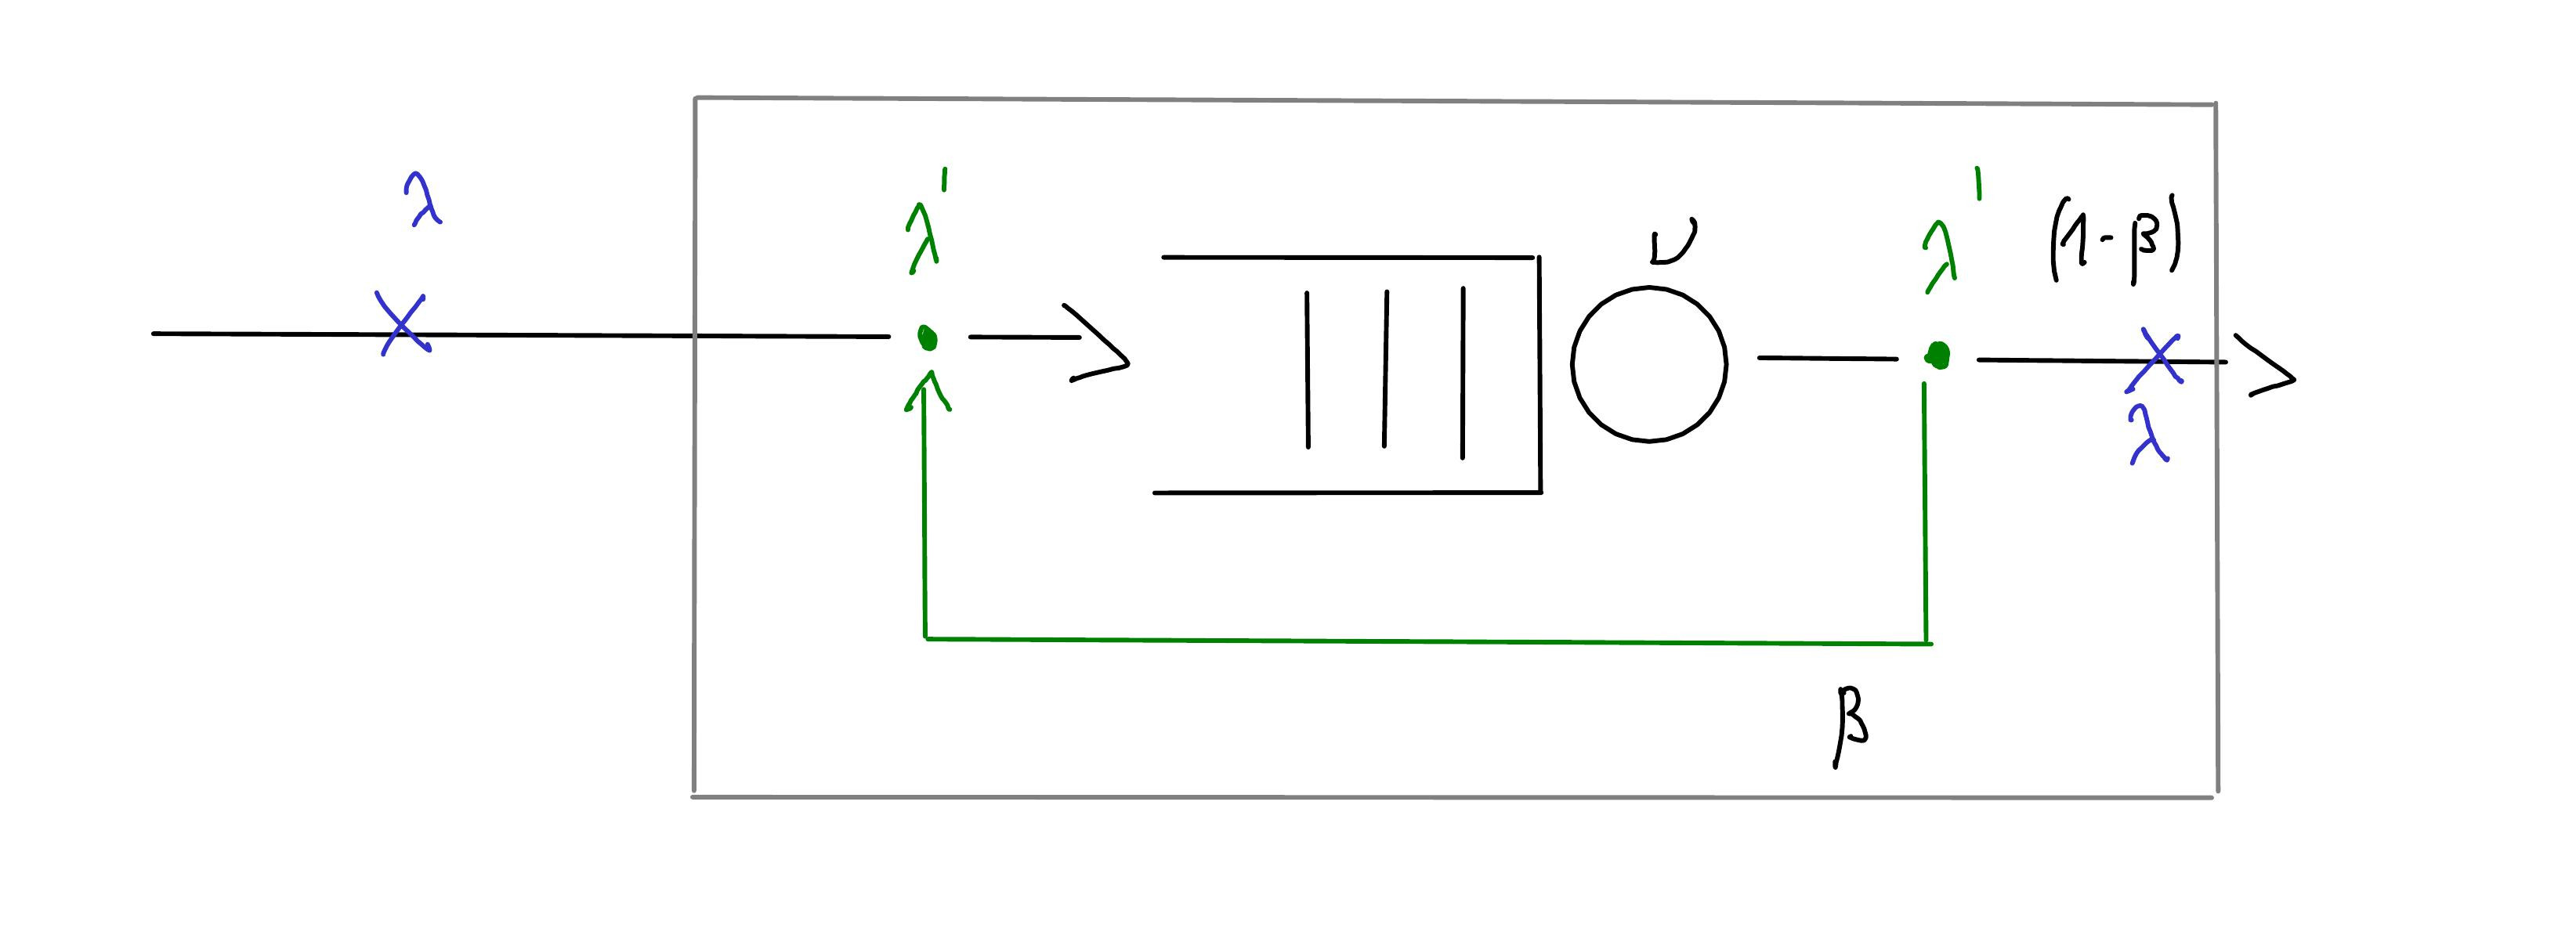
\includegraphics[scale=0.3]{images/PMCSN-1603-1.2.jpeg}\\
a questo punto, le partenze hanno significati diversi dai completamenti: il throughput del server può essere più alto del numero di completamenti, in quanto alcuni possono essere parziali.\\
\\ denotiamo con $\beta$ la probabilità di feedback, ovvero quella con cui un job si rimette in coda (verrà servito in base alla disciplina della coda). Occorre fare delle considerazioni:
\begin{itemize}
\item il feedback è indipendente dalla storia passata, sarebbe diverso se un job sapesse quanti "giri" deve fare quando arriva in coda, assumiamo che sia probabilistico
\item in teoria, un job può fare feedback un numero arbitrario di volte
\item job si mischiano fra quelli che fanno feedback, ma quando calcolo il tempo di risposta i giri fatti da un job devono essere inclusi
\end{itemize}
Vediamo bilanciamento del flusso, throughput etc... L'utilizzazione del centro dipenderà da $\lambda$ e da $\beta$ (non è più $\frac{\lambda}{\nu}$).
\paragraph{Bilanciamento del flusso} deve valere $\lambda = \lambda'(1 - \beta)$, quindi $\rho = \frac{\lambda'}{\nu} = \frac{\lambda}{(1 - \beta)\nu}$ ed il sistema satura quando $\rho \longrightarrow 1$ ovvero quando $\frac{\lambda}{(1 - \beta)\nu} \longrightarrow 1$, in termini di beta quando $\beta \longrightarrow 1 - \frac{\lambda}{\nu}$
\subsection{Analisi del multi-server}
Soluzione del 1917 di Erlang, il modello è M/M/m con scheduling astratto. Anche questa soluzione parte dal determinare la popolazione media nella coda $E(N_Q)_{Erlang}$: si parte con la distribuzione dei job, ovvero la probabilità che nel sistema ci siano N job. Il sistema presenta delle particolarità:
\begin{itemize}
\item il $\rho$ dell'intero sistema è pari al $\rho$ del singolo centro, dove il $\rho$ globale rappresenta la percentuale (sempre a livello stazionario) media di server occupati su un certo periodo di tempo di osservazione
\item il tempo di servizio medio cambia significato: da una parte abbiamo quello del singolo centro, dall'altra quello che passa da quando un job entra in servizio all'istante in cui uno (non è detto che sia lo stesso) esce. I due tempi sono diversi fra loro, il tempo globale è m volte più piccolo del tempo che si spende nel singolo centro.
\end{itemize}
la probabilità che nel centro (coda + m serventi) ci siano n job:
\[
\begin{cases}
p(n) =
\frac{1}{n!}(m \rho)^n p(0) & \text{for } n = 1,...,m\\
\frac{m^m}{m!}\rho^np(0) & \text{for } n > m
\end{cases}
\], dove $p(0) = [\sum\limits_{i=0}^{m-1} \frac{(m \rho)^i}{i!} + \frac{(m\rho)^m}{m!(1 - \rho)}]^{-1}$. \\ L'altra grandezza è $P_Q \cong P(n \geq m)$, ovvero la probabilità che tutti i serve siano pieni, quindi la misura di probabilità che inizi a formarsi la coda: $P_Q = \sum\limits_{n=m}^{\infty} p(n) = \sum\limits_{n=m}^{\infty} \frac{m^m}{m!}\rho^n p(0) = \frac{m^m}{m!p(0)} \sum\limits_{n=m}^{\infty} \rho^n = \frac{m^m}{m!} p(0) \sum\limits_{n=}^{\infty} \rho^{n + m} = \frac{m^m}{m!} p(0) \rho^m \cdot \sum\limits_{n=0}^{\infty} \rho^n$, ma $\sum\limits_{n=0}^{\infty} \rho^n = \frac{\rho}{1 - \rho}$ e quindi $P_Q = \frac{(m\cdot \rho)^m}{m!(1 - \rho)}p(0)$\\ Quindi la popolazione media viene espressa come $E(N_Q)_{Erlang} = P_Q \cdot \frac{\rho}{1 - \rho}$ ed $E(N_S) = P_Q\cdot \frac{\rho}{1 - \rho} + m \rho$. Vale ovviamente la legge di Little, quindi possiamo ottenere $E(T_Q) = \frac{E(N_Q)}{\lambda} \Rightarrow E(T_Q) = P_Q \frac{\rho}{\lambda(1 - \rho)} = \frac{P_QE(S)}{1 - \rho}$.\\ Confrontando con la formula del servente singolo (M/M/1), notiamo una sostanziale somiglianza: qui, il tempo di servizio rimanente in media è il tempo necessario a liberare uno degli m server, quindi NON È $E(S_i)$, perché sarebbe come mettersi in attesa esattamente di uno degli m centro (l'i-esimo specificatamente), IMPORTANTE:è un errore grave fare questo. Si verifica con probabilità $P_Q$ e dura fino ad $E(S)$, ovvero il tempo per liberare uno degli m server.\\ Un'altra grandezza che studiamo è il numero medio di server occupati: chiamiamo la media c: $E(c) = \sum\limits_{n=0}^{m-1} np(n) + \sum\limits_{n=m}^{\infty} mp(n) = m \rho$, ma quindi possiamo riscrivere $\rho$ in altri termini: $\rho = \sum\limits_{n=0}^{m-1} \frac{n}{m}p(n) + \sum\limits_{n=m}^{\infty} p(n)$ ed è ancora uguale a $\sum\limits_{n=0}^{m-1} \frac{n}{m}p(n) + P_Q$ da cui deriviamo che $\rho \geq P_Q$.\\ Da un punto di vista dell'attesa, confrontando multi-server con servente singolo di uguale capacità (tasso $m \mu$, stesso $\lambda$), vediamo che l'attesa è più piccola nel caso del multi-server: nel momento in cui ho m server, è chiaro che l'attesa diminuisce rispetto al singolo; quindi una configurazione del genere consente di avere un tempo medio di attesa più piccola
\subsubsection{Organizzazioni di server} 
Possiamo avere diverse configurazioni:\\
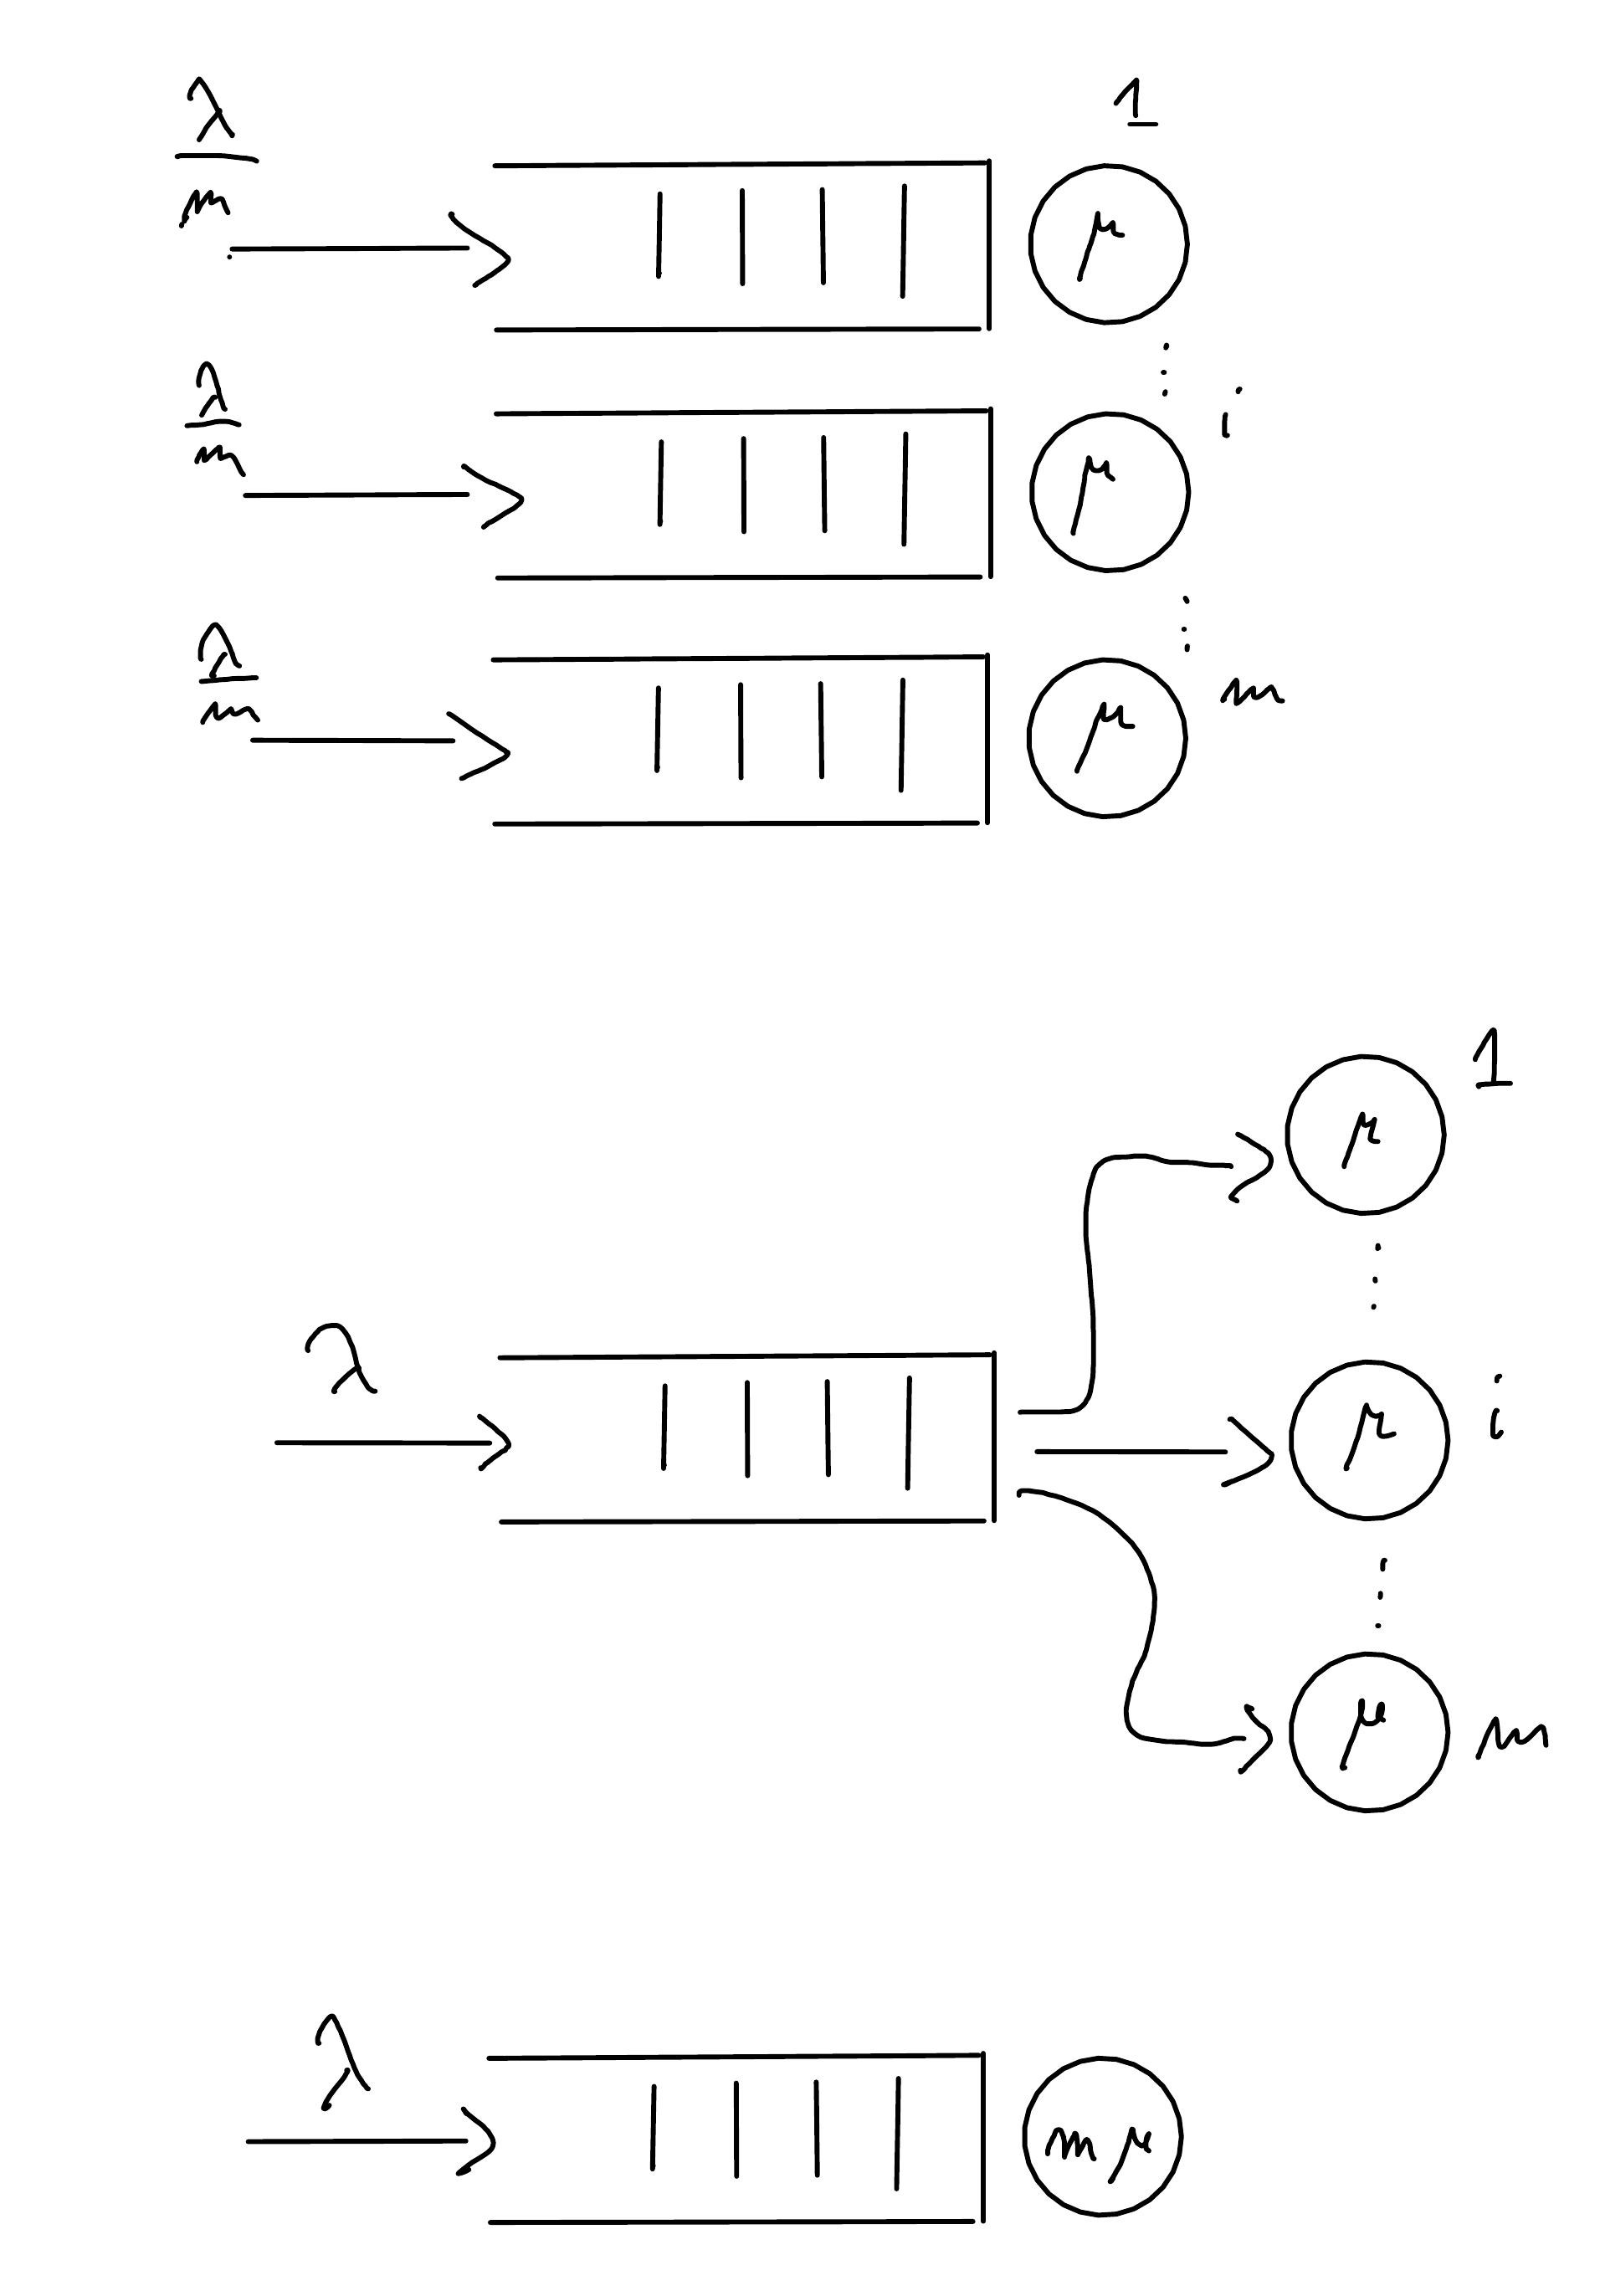
\includegraphics[scale=0.3]{images/PMCSN-1803.jpeg}\\
i $\rho$ delle configurazioni sono le stesse: $\frac{\lambda}{m \mu}$.\\ Le applicazioni sono molteplici:
\\ linee di comunicazione, m linee diverse ed m flussi di Poisson, ognuna con una frequenza di arrivo $\frac{\lambda}{m}$ pacchetti per secondo. La distribuzione dei servizi è una $Exp(\frac{1}{\mu})$. Nella gestione dei canali di comunicazione ci sono due diversi approcci:
\begin{itemize}
\item frequency division multiplexing (o time): sporziono la frequenza in m frequenza di uguale capacità, quindi è il primo modello visto
\item statistical multiplexing: condivido la capacità comunicativa, quindi c'è il merge degli m originali in un unico flusso, quindi il modello sarà il 3°.
\end{itemize}
la domanda può essere come i due diversi approcci si comportano da un punto di vista del tempo medio di risposta: nel caso di una M/M/1, abbiamo $E(T_S) = \frac{\rho E(S)}{1 - \rho} + E(S) = \frac{E(S)}{1 - \rho}$, da cui $E(T_S) = \frac{1}{\mu - \lambda}$. Nei 3 casi,tutti i centri sono M/M/1, quindi per $E(T_S) = \frac{m}{m \mu - \lambda}$ nel caso del FDM. Nel caso dello statistical multiplexing abbiamo $E(T_S) = \frac{1}{m \mu - \lambda}$, quindi FDM ha un tempo medio di risposta m volte più grande dello SM.\\ Ma il FDM da una garanzia di qualità per ogni flusso, quindi se abbiamo una QoS da rispettare, con il FDM siamo tranquilli di poter garantire ad ogni flusso una frequenza di servizio che è $\mu$, mentre nel caso dello SM non c'è questa sicurezza.\\ Inoltre, se noi avessimo dei flussi molto regolari (non di Poisson), andando a fare il merge si perde questa regolarità: andiamo ad introdurre unac erta variabilità, che potrebbe non andare bene per applicazioni che richiedono una bassa variabilità (es: traffico voce o video).\\ Rimane il confronto fra il 2° ed il 3° modello, ricorda uno degli esempi fatti inizialmente, sui server di capacità differenti, in cui volevamo un tempo medio di risposta basso. Dipende dalle assunzioni: se i job sono non preemptible:
\begin{itemize}
\item se la variabilità è alta, si preferisce il 2° modello. Vogliamo evitare che job grandi blocchino i piccoli
\item se la variabilità è bassa, sarebbe da preferire il 3° modello. Se $\rho$ è basso, con una capacità non contentata le risorse sarebbero sprecate
\end{itemize}
indipendentemente dall'assunzione, se l'obiettivo è minimizzare il tempo medio di risposta ed è possibile fare preemption, allora possiamo sempre simulare il comportamento del 2° sistema col 3°: possiamo interrompere un job grande all'arrivo di uno piccolo, diamo servizio a quest'ultimo e poi riprendiamo; tutti i job usufruiscono di capacità elaborativa maggiore e c'è anche fairness.\\ Vediamo tutto questo nell'analisi:
\begin{itemize}
\item tempo di attesa: $E(T_Q)_{Erlang} = \P_Qfrac{E(S)}{1 - \rho}$, mentre $E(T_Q)_{KP} = \frac{\rho E(S)}{1 - \rho}$
\item da un punto di vista del tempo di risposta $E(T_S)_{Erlang}$, dobbiamo sommare il tempo di servizio che è $E(S_i)$, perché $E(T_S)_{Erlang}$ modella il tempo che passa da quando il job arriva a quando prende servizio presso uno dei job; a quel punto sarà servito con tasso $\frac{1}{\mu}$.
Otteniamo quindi: $E(T_S)_{Erlang} = \frac{P_Q E(S)}{1 - \rho}+E(S_i)$ ed $E(T_S)_{KP} = \frac{\rho E(S)}{1 - \rho} + E(S)$, notare che $E(S_i) = \frac{1}{\mu} = m \frac{1}{m \mu} = mE(S)$. Confrontando i due termini, il risultato dipenderà dal valore di $\rho$:
\begin{itemize}
\item $\rho \longrightarrow 1$, le prestazioni tendono a convergere, i server saranno sempre molto pieni quindi approssimativamente hanno lo stesso tempo di risposta
\item $\rho \longrightarrow 0$ la configurazione 2° da prestazioni m volte più lente
\end{itemize}
\end{itemize}
dipende quindi tutto dall'obiettivo che si ha.\\ Dal confronto fra servente singolo e multi-server (con m = 5), emergono alcuni risultati:
\begin{itemize}
\item Tempo di attesa: al tendere di $\rho$ ad 1, le due curve tendono allo stesso asintoto verticale.
\item Tempo di risposta, le cose cambiano completamente: ATTENZIONE: nel tempo di risposta si somma la tempo di attesa il tempo di servizio che il job dovrà mediamente spendere. Nel caso del multi-server, per avere una capacità globale equivalente, questo tempo è m volte più lento ed è quello che pesa di più nel requisito di qualità\footnote{in questo caso il tempo di risposta più piccolo} 
\end{itemize}
\subsubsection{Fattore di scala}
Cosa succede se le specifiche del nostro problema vengono aumentate entrambe di un fattore a: $\lambda \rightarrow a\lambda$ e $\mu \rightarrow a\mu$, Abbiamo visto che i tempi si riducono dello stesso fattore a. Consideriamo sempre i due sistemi di prima, siamo sempre a parità di $\rho$:
\begin{itemize}
\item tempo medio di attesa: $E(T_Q)_{m,a} = \frac{P_Q E(S)_{m,a}}{1 - \rho} = \frac{P_Q}{ma \mu (1 - \rho)} = \frac{1}{a}\cdot \frac{P_Q E(S)_{m,1}}{1 - \rho}$ = $\frac{1}{a}\cdot E(T_Q)_{m,1}$ 
\item tempo medio di risposta
\end{itemize}
\subsubsection{Confronti numerici}
Confrontiamo ancora tutti e 3 i modelli, per confermare con i numeri le prestazioni:\\
FDM: $\lambda = 4 j/s, m = 4, \mu = 1.5 j/s, E(S) = 0.666667 s$, abbiamo un $\rho = 0.666667$, assumiamo tempo di servizio esperienziale, otteniamo un $E(T_S) = \frac{1}{\mu - \lambda} = 2 s$\footnote{dove il $\lambda$ è quello del singolo centro, quindi $\frac{\lambda}{4}$}, mentre per $E(T_Q) = \frac{\rho E(S)}{1 - \rho} = 1.3336 s$.\\ Confrontando con il multi-server, abbiamo un $E(S) 0 0.1667$, stesso $\rho$, con la Erlang otteniamo $p(0) = [(\sum\limits_{i=0}^{3} \frac{(4 \rho)^i}{i!}) + \frac{(4 \rho)^4}{4!(1 - \rho)}]^{-1} = 0.059857$. La $p(0)$ è la probabilità che il centro sia completamente vuoto, sia in coda che in servizio, quindi da un punto di vista stazionario se osserviamo il sistema per un periodo di tempo abbastanza lungo, la percentuale di tempo in cui lo osserviamo vuoto è circa del 6\%. Otteniamo quindi una $P_Q = \frac{(4 \rho)^4}{4!(1 - \rho)}p(0) = 0.37847$, ovvero la probabilità che tutti i centri siano pieni è del 38\% circa, $E(T_S) = \frac{P_Q\cdot E(S)}{1 - \rho} + E(S_i)$, sommo $E(S_i)$, misura da quando un job arriva in coda a quando prenderà servizio e quando lo farà spenderà in media $E(S_i)$ e non $E(S)$, infine $E(T_Q) = 0.189292 s$.\\ Quindi ora concentriamo anche gli m$\mu$: $m \mu = 4\cdot 1.5 j/s, E(S) = 0.166667s$, usando la KP calcoliamo $E(T_S) = \frac{1}{m \mu - \lambda} = 0.5$, $E(T_Q) = 0.3334 s$. Quindi nel confronto finale, il tempo minimo di attesa è nel multi-server, poi si passa al concentrato ed infine al FMD, in cui abbiamo garanzie sul QoS a scapito di prestazioni decisamente peggiori.\\ Da un punto di vista del tempo di attesa le cose cambiano: il 3° modello ha il minimo, poi abbiamo il multi-server e poi il 1° caso.
\section{Processi di Markov}
\subsection{Storia di Google}
L'algoritmo dietro al motore di ricerca è PageRank: l'idea è stata quella di risolvere il problema ricorsivamente, usando un formalismo modellistico che assegnava un rank (peso) ad una pagina a seconda di quant'era la somma dei punteggi che avevano le pagine che la puntavano. Ogni pagina aveva un rank, che dipendeva dai ranking di quelle che vi puntavano. Rank j $\approx prob \pi_j$, dove $\pi_j = \sum\limits_{i=1}^{n} \pi_i$. L'algoritmo prevedeva la creazione di una catena di Markov a stati discreti dove ogni stato era un pagina web con connessioni per le pagine linkate.\\ Se una pagina i è collegata a k pagine, la probabilità di spostarsi da quella pagina ad una delle k, la probabilità di sposarsi era uniforme $\frac{1}{k}$.\\ Risolvendo la catena, le pagine erano presentate in base alle loro probabilità limite, quindi in ordine in base al loro rank. Ci sono una serie di problemi se la cosa fosse risolta solo così:
\begin{itemize}
\item le pagine possono essere facilmente create, quindi si potrebbero creare 1000 pagine che puntano alla loro
\item pagine trap, ovvero che non puntano ad altre pagine
\end{itemize}
ci sono quindi una serie di raffinamenti che tengono conto di tutti i problemi
\subsection{Elementi per un processo di Markov}
Processo stocastico: possiamo definirlo come un insieme di variabili aleatorie che ha come indice il parametro tempo, ne consideriamo varie istanze (outcome): \{$X(t_1), X(t_2),...$\}\\ Lo spazio degli stati ci dice i valori ammissibili che la famiglia di v.a può assumere: \{$s_0, s_1,...$\}\\ La catena di Markov è un particolare processo stocastico che gode della stessa memoryless property per cui l'evoluzione delle v.a nel tempo non determinano nulla rispetto all'evoluzione futura, ma l'insieme informativo è tutto contenuto nello stato all'istante t. Ne definiamo la probabilità come : $P\{X(t_{n+1}) = x_{n+1}|X(t_n) = x_n, X(t_{n-1}) = x_{n-1},...,X(t_0) = x_0\} = P\{X(t_{n+1}) = x_{n+1}|X(t_n) = x_n\}$. Siamo molto interessati alle distribuzioni a fasi, ad esempio alla Cox, in quanto abbiamo diversi stati che ci rappresentano le fasi di servizio, che è esponenziale e quindi può essere modellata con Markov. Se il job esce, bisogna vedere cosa accade, comunque il sistema transita in un nuovo stato, se invece il jbo continua, il processo stocastico che modella l'evoluzione del servizio, passa da uno stato esponenziale ad un altro sempre esponenziale; quindi il processo stocastico continua ad essere di Markov, pur in presenza di distribuzioni del servizio così generali.
\paragraph{Distribuzione di probabilità istantanea}definita come $P\{X(t) = s_i\} = \pi(s_i,t)$. Si dimostra che quando lo spazio degli stati è finito, il processo è irriducibile\footnote{irriducibile: non ci sono stati da cui non è possibile uscire, quindi al limite la probabilità dello stato sarebbe 1} ed ergodico, esiste $\lim_{t\rightarrow \infty} \pi(s_i,t) = \pi(s_i)$.
\paragraph{Probabilità stazionaria}immagino che lo spazio degli stati sia finito, li poniamo sull'asse x, sulle ordinate abbiamo la probabilità dello stato al tempo t\\
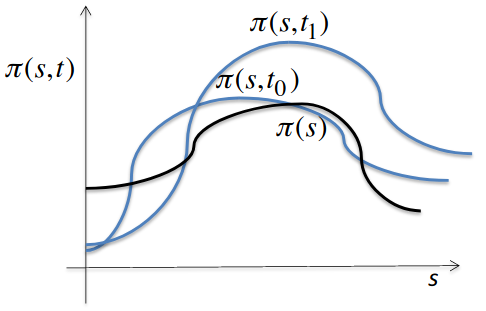
\includegraphics[scale=0.3]{images/PMCSN-2303.png}\\
Studiamo il sistema e capiamo le condizioni iniziali\footnote{ovvero al tempo $t_0$}, poi al tempo $t_1$, notando che la probabilità è cambiata, perché magari il sistema evolve in un certo modo. Possiamo vedere dopo quanto tempo si tende ad una probabilità stazionaria, ovvero dalla quale non ci si muove più al trascorrere del tempo: anche se passa altro tempo, il sistema non cambia probabilità. Questo è fondamentale nella simulazione, nel caso in cui siamo interessati alla stazionarietà: se dobbiamo raccogliere un campione, occorre capire da quale punto in poi il campione rappresenta lo stato stazionario
\subsection{Server a singolo centro con coda finita}
Se la coda è piena, alcuni arrivi vengono perduti, quindi il throughput e l'utilizzazione cambiano, è necessario un processo di Markov. Da un punto di vista della modellazione, le cose cambiano: supponiamo che la capacità del sistema sia C\footnote{coda + servizio}, il processo X(t) rappresenta in numero di job nel centro. Siccome ho capacità finita, questo \textbf{garantisce che la stazionarietà c'è sempre}: la coda è finita, quindi del tasso di arrivo si perde ed il server si troverà a smaltire C, ed al tendere del tempo all'infinito riuscirà sempre a smaltire C:\\ 
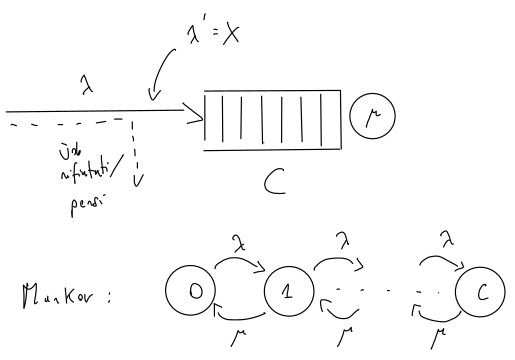
\includegraphics[scale=0.5]{images/PMCSN-2403-2.jpeg}\\
da ogni stato si passa nel successivo con tasso $\lambda$, mentre si torna indietro di stato con tasso $\mu$.\\ Come avviene la risoluzione: scriviamo stato per stato \textbf{l'equazione di bilanciamento globale}, stiamo considerando la stazionarietà:
\begin{itemize}
\item $\pi_0 \cdot \lambda = \pi_1 \cdot \mu$, ci deve essere un equilibrio fra i flussi che entrano e quelli che escono , altrimenti non avrei la stazionarietà, da qui possiamo ricavare $\pi_1 = \frac{\lambda}{\mu}\pi_0$
\item $\pi_1(\lambda + \mu) = \pi_0 \lambda + \pi_2 \mu$, qui le cose cambiano, in quanto nello stato 1 posso entrare ed uscire in diversi modi. Anche qui, possiamo ricavare $\pi_2 = (\frac{\lambda}{\mu})^2 \pi_0$
\end{itemize}
quindi avremo: $\pi_C = (\frac{\lambda}{\mu})^C \pi_0$, e per il generico i $\pi_i = (\frac{\lambda}{\mu})^i \pi_0$. Dobbiamo avere che $\sum\limits_{i=1}^{C} \pi_i = 1$ (condizione di normalizzazione), da qui possiamo ricavare $\pi_0 = \frac{1}{\sum\limits_{i=0}^{C} (\frac{\lambda}{\mu})^i}$. Qual è la probabilità di perdita: $\pi_C = (\frac{\lambda}{\mu})^C \pi_0 = \frac{(\frac{\lambda}{\mu})^C}{\sum\limits_{i=0}^{C} (\frac{\lambda}{\mu})^i}$, quindi il tasso di ingresso reale è $\lambda' = \lambda(1 - p_{loss})$ da cui $\rho = \frac{\lambda'}{\mu}$.\\ esempio: C = 4, $\lambda = \mu = 5 j/s$, la capacità finita fa sì che il sistema si stabilizzi sempre. Da quanto visto prima, abbiamo che $\pi_i = (\frac{\lambda}{\mu})^i \pi_0$, tutti i $\pi_i$ saranno pari ad $\frac{1}{5}$ (andando ad intersecare con la condizione iniziale $\sum\limits_{i=0}^{4} \pi_i = 1$. La $p_{loss} = \pi_4 = \frac{1}{5}$, da cui $\lambda' = \lambda(1 - p_{loss}) = 4 = X$ e $\rho = 0.8$
\subsection{M/M/m/m - m server loss system}
Abbiamo un certo numero di risorse parallele, senza alcun buffer delle richieste: quindi, o le richieste trovano subito un server libero, oppure si perdono (ad esempio: chiamate telefoniche o connessioni con circuiti virtuali). Ipotizziamo una distribuzione del servizio esponenziale, la soluzione (di Erlang) usa le catene di Markov: \\
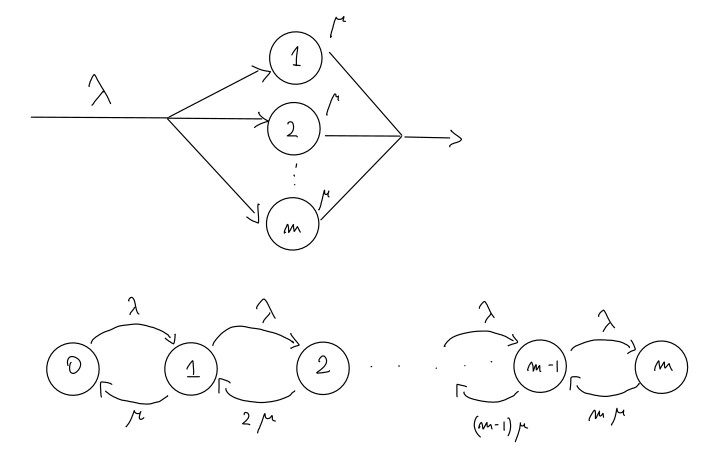
\includegraphics[scale=0.5]{images/PMCSN-2403-1.jpeg}\\ 
a seconda del livello di occupazione del server, il tasso di servizio sarà pari a $i \mu$. Abbiamo $\pi_i = (\frac{\lambda}{\mu})^i \frac{1}{i!}\pi_0$, unendo con la somma delle probabilità $\sum\limits_{i=0}^{m} \pi_i = 1$ otteniamo $\pi_0 = \frac{1}{\sum\limits_{i=0}^{m} (\frac{\lambda}{\mu})^i \frac{1}{i!}}$, da cui otteniamo $\pi_i = \frac{(\frac{\lambda}{\mu})^i}{i! \sum\limits_{j=0}^{m} (\frac{\lambda}{\mu})^j \frac{1}{j!}}$, tale formula prende il nome di Erlang-B, lo stato m è la probabilità di perdita, ovvero la percentuale di tempo in cui il sistema perderà richieste in ingresso. Confrontando con la Erlang-C, a parità di $\lambda, \mu, m$: $\pi_m = (\frac{\lambda}{\mu})^m \frac{1}{m!} \pi_0$ vs $P_Q = \frac{(m \rho)^m p(0)}{(\frac{\lambda}{\mu})^m m!(1 - \rho)} = \frac{(\frac{\lambda}{\mu})^m}{m!(1 - \rho)p(0)}$. Ora, la parte $\frac{(\frac{\lambda}{\mu})^m}{m!(1 - \rho)}$ è sicuramente maggiore di $\frac{(\frac{\lambda}{\mu})^m}{m!}$, ed intuitivamente, la presenza della coda rende $\pi_0 > p(0)$.\\ esempio: $\lambda = 5 j/s$, $\mu = \frac{1}{300} j/ms = 3.33333 j/s$, $m = 4 \Rightarrow m \mu > 12 j/s$, abbiamo una $p_{loss} = \pi_4 = 0.048$, $\lambda' = \lambda(1 - p_{loss}) = 4.76 j/s$ con un $\rho = \frac{\lambda'}{\mu} = 0.357$.
\section{Introduzione alla simulazione}
Cambia il tipo di approccio per la valutazione delle prestazioni, per caratterizzare un modello di simulazione ci sono diverse tipologie, tutti i sistemi hanno una qualche componente stocastica, differenza fra modello statico e dinamico: nel primo la variabile tempo non è significativa, mentre nel secondo si. Il caso di nostro interesse è un sistema con componente stocastica, dinamica e discreta. Come si sviluppa un modello: non ci sono tecniche automatiche, ce ne sono per delle classi particolari e limitate, in generale si parla di "arte" dello sviluppo dei modelli di valutazione. Occorre seguire una serie di passi, saltarne alcuni porta al fallimento dello sviluppo della valutazione. Quali sono i primi passi:
\begin{itemize}
\item obiettivi dello studio: sono fondamentali, possono essere espressi come decisioni booleane, numeriche etc...
\item sviluppo del modello concettuale
\item convertire il modello concettuale in modello delle specifiche
\item convertire il modello delle specifiche nel modello computazionale: il modello computazionale sarà lo sviluppo del simulatore se si parla di modello simulativo, altrimenti un solutore della catena di Markov se siamo in un modello analitico
\item verifica
\item validazione
\end{itemize}
Sul primo punto, gli obiettivi non devono condizionare le scelte nella fase di sviluppo del modello.\\ Ci sono 3 livelli di modelli:
\begin{itemize}
\item[i] modello concettuale: a livello alto, occorre cercare di definire quali sono le variabili di stato essenziali per quel sistema sotto quegli obiettivi. Quali sono le variabili di stato possono essere ignorate per semplificare il modello, come le variabili sono collegate fra loro
\item[ii] modello delle specifiche: viene fatta sostanzialmente su carta, può coinvolgere pseudocode, equazioni etc... Cosa riceverà il modello come input? Raccogliamo ed analizziamo l'input usando dei modelli stocastici rappresentativi. Vedremo più che altro le tecniche, occorre capire 
\item[iii] modello computazionale: sviluppo del codice che serve per la soluzione, un'altra filosofia è se usare linguaggi general purpose o specifici per la simulazione: il simulatore è un oggetto relativamente complesso, ha una serie di debolezze a cui occorre prestare attenzione, gli strumenti "black box" sono rischiosi; quindi si sceglie un linguaggi general purpose.
\end{itemize}
\paragraph{Verifica vs validazione} la verifica occorre per capire se, rispetto al modello che avevo, ciò che ho implementato è corretto o no. Ma ciò non mi dice nulla rispetto al sistema reale, ovvero se il modello è una buona rappresentazione di quel caso di studio oppure no. Verifica: ho costruito il modello correttamente? Validazione: ho costruito il modello giusto rispetto a quel sistema?\\ Il processo è iterativo, alcune osservazioni:
\begin{itemize}
\item cerchiamo di avere modelli quanto più semplici possibili, ovvero che non ci sia un modello più semplice di quello trovato, che comunque non deve né ignorare delle caratteristiche, né includerne troppe
\item lo sviluppo non è sequenziale, se si lavora in team si possono fare degli step in parallelo. ATTENZIONE: non si mischiano verifica e validazione
\item NON si saltano i passi per passare alla programmazione
\end{itemize}
C'è una seconda parte dell'algoritmo, che riguarda la progettazione degli esperimenti:
\begin{itemize}
\item progettazione di esperimenti di simulazione
\item fare delle run, conservando dati di input e condizioni iniziali
\item analisi dell'output: dai risultati ottenuti, occorre tirare fuori delle linee guida, verso che tipo di soluzioni andare. L'analisi statistica dei risultati della simulazione è più difficile della statistica classica: viene meno l'indipendenza fra le v.a, occorre che il campione abbia delle caratteristiche che permettono di applicare i metodi statistici
\item prendere delle decisioni: dal passo precedente, bisogna decidere cosa fare. Prima di mettere in atto le decisioni, potremmo simulare quali sarebbero le conseguenze delle azioni che stiamo pensando di applicare, potremmo modificare il simulatore per poter includere le politiche che migliorano le prestazioni del sistema
\item documentazione dei risultati: la simulazione è uno studio prezioso, costoso, quindi è un know-how prezioso. \textbf{Se non è ben documentato, so cazzi:} importante avere una documentazione ben fatta sia del codice, sia sulle linee guida generali che sono state raggiunte
\end{itemize}
\subsection{Machine stop model}\label{machine}
Problema di failure di macchine. 150 macchine identiche che operano continuativamente:
\begin{itemize}
\item 8 h/giorno
\item 250 g/anno
\end{itemize}
Operano indipendentemente, vengono riparate se falliscono. Guadagno è di 50000 €/h per macchina. Per la riparazione, viene assunto un servizio tecnico:
\begin{itemize}
\item contratto di 2 anni, 60000 €/anno
\item ogni tecnico lavora 230 g/anno per 8 h/giorno
\end{itemize}
Quanti tecnici dovrebbero essere assunti per massimizzare il profitto? È utile pensare ai casi limite:
\begin{itemize}
\item unico tecnico: l'overhead del servizio tecnico è minimizzato, ma i tempi di attesa per la riparazione cresceranno moltissimo, quindi ci doverebbe essere una grande perdita di profitto
\item numero di tecnici pari al numero di macchine: overhead tecnico enorme, è probabilmente il minimo caso di donwtime, il profitto dovrebbe massimizzarsi, ma c'è l'overhead dei tecnici
\end{itemize}
\paragraph{Modello concettuale}il modello concettuale: deve sicuramente includere:
\begin{itemize}
\item lo stato di ogni macchina
\item lo stato di ogni tecnico
\item dovrà dare lo stato del sistema a ciascun istante di tempo
\end{itemize}
modello ibrido: ci sono degli elementi del modello analitico\\ A livello di specifiche, occorre chiedersi alcune cose:
\begin{itemize}
\item sappiamo dopo quanto tempo una macchina si guasta di nuovo? I guasti sono random? Se lo fossero, il tempo inter-guasto sarebbe esponenziale
\item sappiamo qualcosa sui tempi di riparazione? C'è una distribuzione che rappresenta bene i tempi?
\item come verrà simulata la distribuzione temporale
\end{itemize}
\paragraph{Modello computazionale}nel modello computazionale, dovrà esserci una struttura dati per le macchine guaste ed anche per i tecnici disponibili. Dovranno anche essere incluse tutte le strutture dati per collezionare la variabili di output.
\paragraph{Verifica}la fase di verifica è una tipica attività di ingegneria del software, solitamente viene fatta mediante testing, è possibile anche usare dei controlli di consistenza.
\paragraph{Validazione}la fase di validazione tende a stabilire quanto il modello deciso ed implementato è rappresentativo del sistema reale: la maniera migliore di validare un modello, sarebbe quella di confrontarsi con il caso reale ma non è sempre possibile. Quindi, si possono eseguire controlli di consistenza, per verificare che il simulatore abbia lo stesso comportamento del sistema reale.\\ Se il caso di studio lascia pensare (rispetto al modello delle specifiche) che la soluzione analitica è coerente, quindi ha un certo livello di affidabilità, lo stesso modello analitico potrebbe anche costituire in parte una validazione: se il simulatore da la stessa soluzione, possiamo fidarci che il simulatore è abbastanza rappresentativo.
\paragraph{Progetto degli esperimenti}l'obiettivo è quello di trovare l'ottimo numero di tecnici, quindi occorrerà fare riferimento a valori parametrici. Partiamo da alcune condizioni iniziali, ad esempio che inizialmente tutte le macchine all'istante 0 sono operative.\\ A questo punto, per ogni set di parametri bisogna capire quanti run di simulazione occorrono: un unico run rappresenta uno scenario particolare.\\
\paragraph{Runs}la gestione dell'output può diventare un problema, una simulazione produce una quantità di dati molto grande. Evitare di memorizzare dati grezzi, siccome la simulazione è replicabile, è possibile ripetere un particolare esperimento di simulazione.
\paragraph{Analisi dell'output}è più complicata dell'analisi statistica classica (dove avevo il mio simple random sample con le sue proprietà), se stiamo guardando il numero di macchine guaste durante una simulazione su un intervallo di tempo significativo è abbastanza probabile che due osservazioni successive siano correlate: rispetto a quello che dovrebbe essere il valore medio, potrebbero essere entrambe sopra o sotto la media.\\ Due osservazioni saranno vicine temporalmente ed avranno una certa correlazione
\paragraph{Fase di decisione}la rappresentazione grafica dell'output della simulazione aiuta, ad esempio abbiamo un grafico in cui da un lato c'è il profitto, dall'altro il fatto che avere pochi tecnici porterebbe ad avere più macchine guaste. Ci immaginiamo una curva che parte bassa, poi sale e poi scende: possiamo vedere l'ottimo (se è un massimo assoluto) ed anche la sensitività negli intorni di quest'ottimo
\paragraph{Documentazione} dovrà includere una visione del diagramma del sistema, che sia comunicabile anche a non esperti, tutte le tabelle grafici, il software, le assunzioni e la descrizione dell'analisi dell'output.\\ Un'altra caratteristica interessante della modellazione è che ci permette di capire delle cose che altrimenti non sarebbe possibile ottenere.
\section{Simulazione trace-driven}
Vediamo l'applicazione al caso di studio 1, introdotto nella \ref{machine}. Partiamo con terminologia:
\begin{itemize}
\item coda/centro/nodo sono sinonimi
\item job/richiesta/utente sono sinonimi
\end{itemize}
da un punto di vista di tempi:
\begin{itemize}
\item tempo di attesa, come usato fin ora, rappresenta il tempo che passa dall'istante in cui arriva finché non prende servizio. Nel libro, il tempo di attesa è indicato con \textit{delay}, ovvero in ottica del ritardo che subisce la richiesta
\item il tempo di risposta viene chiamato \textit{wait}
\end{itemize}
Per un job i, in un centro con singolo server e singola coda teniamo traccia di:
\begin{itemize}
\item tempo di arrivo $a_i$
\item tempo di servizio $s_i$
\item delay in coda $d_i$
\item istante in cui comincia il servizio: $b_i = a_i + d_i$
\item tempo di wait: $w_i = d_i + s_i$
\item tempi di partenza: $c_i = a_i + w_i$ (completamento)
\end{itemize}
$a_i, s_i$ sono variabili di input, tutte le altre sono variabili di output.\\ Il tempo di inter-arrivo fra i job $j_{i-1}$ e $j_i$ è indicato come $r_i = a_i - a_{i-1}$, dove per definizione $a_0 = 0$, assumiamo che non ci siano bulk arrivals, ovvero che ad ogni istante di tempo ci sia un solo arrivo (probabilità di attivi simultanei prossima allo 0), tutti gli $r_i > 0 \forall i$.
\subsection{Trace driven simulation}
Il modello è guidato dai dati esterni di input, noi abbiamo $a_i$ ed $s_i$, come possiamo calcolare il tempo di coda $d_i$: per alcune discipline di coda, non è semplice. Ma se ci limitiamo al caso FIFO, $d_i$ è determinato da quando $a_i$ avviene rispetto a $c_{i-1}$, ovvero rispetto all'ultimo completamente. A seconda se avvenga prima o dopo, ci saranno risultati diversi:
\begin{itemize}
\item il job arriva prima che il precedente completi, ovvero $a_i < c_{i-1}$
\item se invece $a_i > c_{i-1}$, il job i-esimo prende subito servizio (perché trova il centro vuoto) e quindi il tempo di delay è $d_i = 0$.
\end{itemize}
Queste equazioni vengono determinate a livello di specifiche e modello concettuale, in cui si capiscono le relazioni.
\subsubsection{Statistiche di output}
Da un punto di vista di definizione analitico, le statistiche di output si dividono in due tipologie:
\begin{itemize}
\item job average: il tempo medio di inter-arrivo $\bar{r} = \frac{1}{n} \sum\limits_{r_i} = \frac{a_n}{n}$, quindi il tasso di arrivo ($\lambda$) è $\frac{1}{\bar{r}}$. Da un punto di vista empirico, è abbastanza chiaro quant'è il tempo di inter-arrivo medio: prendo il numero di arrivi avuti fino a quel momento e divido per n.\\ Analoga operazione per il tempo di servizio medio: $\bar{s} = \frac{1}{n} \sum\limits_{s_i}$. L'attesa e la risposta media: $\bar{d} = \frac{1}{n} \sum\limits_{d_i}$ e $\bar{w} = \frac{1}{n} \sum\limits_{w_i}$. Poiché $w_i = d_i + s_i$, la relazione vale anche per le medie. Quindi, dai dati in input è possibile calcolare le medie, e viste le relazioni di dipendenza basta calcolarne due e derivare la terza. Ma sarebbe buona norma calcolare tutti i valori indipendentemente e poi fare la verifica come controllo di consistenza usare la relazione.
\item time average: statistiche legate alle popolazioni:
\begin{itemize}
\item l(t): popolazione media nel sistema al tempo t
\item q(t): popolazione media nella coda al tempo t
\item x(t): numero medio di job in servizio al tempo t
\end{itemize}
per definizione: l(t) = q(t) + x(t) $\forall t$. Sono tutte funzioni a gradino, siccome assumono valori interi.
\end{itemize}
Supponiamo di guardare un intervallo $(0, \tau)$:
\begin{itemize}
\item il numero medio nel tempo in coda è dato da $\bar{l} = \frac{1}{\tau} \int\limits_{0}^{\tau} l(t) dt$
\item media nel tempo in coda $\bar{q} = \frac{1}{\tau} \int\limits_{0}^{\tau} q(t) dt$
\item media nel tempo in servizio $\bar{x} = \frac{1}{\tau} \int\limits_{0}^{\tau} x(t) dt$, è anche l'utilizzazione. Per definizione di utilizzazione, è chiaramente minore di 1
\end{itemize}
sono tutte collegate con la legge di Little: come visto nella \ref{Little}, le ipotesi valgono e quindi abbiamo: $\int\limits_{0}^{c_n} l(t) dt = \sum\limits_{i=1}^{n} w_i$, dove $c_n = \tau$. Lo stesso si può dire a livello di coda e di servente: $\int\limits_{0}^{c_n} q(t) dt = \sum\limits_{i=1}^{n} d_i$, $\int\limits_{0}^{c_n} x(t) dt = \sum\limits_{i=1}^{n} s_i$, dove $c_n = \tau$. Se noi andiamo a scriverci la funzione cumulativa degli arrivi e la funzione cumulativa delle partenze, abbiamo una corrispondenza con il tempo che ogni job richiede: quando calcoliamo l'aera, stiamo calcolando il tempo di risposta del job. Quindi integrando su tutto il tempo equivale a fare la somma di tutti i tempi di risposta per tutti i job.\\ $\tau$ corrisponde a $c_n$, quindi sostituendo: $\bar{l} = \frac{1}{\tau} \int\limits_{0}^{\tau} l(t) dt = c_n \bar{l} = \int\limits_{0}^{c_n} l(t) dt$, usando Little abbiamo $\sum\limits_{i=1}^{n} w_i = n \bar{w}$, da cui $\bar{l} = \frac{n}{c_n} \bar{w}$ lo stesso vale per $\bar{q} = \frac{n}{c_n} \bar{d}$, $\bar{x} = \frac{n}{c_n} \bar{s}$.\\$\frac{n}{c_n}$: n job completano in $c_n$, quindi otteniamo il throughput in $c_n$; nel caso della coda infinita, corrisponde alla frequenza media di arrivo.
\paragraph{Intensità di traffico}il rapporto fra la frequenza di arrivo e la frequenza di servizio $\dfrac{\frac{1}{\bar{r}}}{\frac{1}{\bar{s}}} = \frac{\bar{s}}{\bar{r}} = \frac{\bar{s}}{\frac{a_n}{n}} = (\frac{c_n}{a_n})\bar{x}$ questo poiché $\bar{x} = \frac{x}{c_n}\bar{s}$. Questo per dire che la frequenza di servizio coincide con l'utilizzazione soltanto quando il rapporto $\frac{c_n}{a_n}$ tende ad 1, ma per periodi di tempo piccoli (quindi piccole finestre temporali) l'utilizzazione coincide con l'intensità di traffico quando il tempo di simulazione è sufficientemente lungo.
\subsubsection{Algoritmo}
Algoritmo:
\lstset{
	mathescape
}
\begin{lstlisting} 
$c_0$ = 0.0;
i = 0;
while (more jobs to process){
	i++;
	ai = GetArrival();
	if($a_i < c_{i-1}$)$d_i = c_{i-1} - a_i$;
	else $d_i = 0.0$;
	$s_i$ = GetService();
	$c_i = a_i + d_i + s_i$;
	}
	n = 1;
	return $d_1, d_2, ... , d_n$;
\end{lstlisting}
\textit{GetArrival()} e \textit{GetService()} leggeranno da file, prendendo i primi tempi. Possiamo calcolare il tempo di inter-arrivo medio, il tempo di servizio medio etc... a partire dai dati e dai valori dei $d_i$ risultanti dopo la simulazione. È possibile calcolare la media dei delay $\bar{d_i}$, siccome occorre dover effettuare la verifica e questo può essere complicato, un approccio può essere quello di calcolare i valori e poi usare l'equazione $\bar{w} = \bar{d} + \bar{s}$ per fare la verifica.
\subsubsection{Case study - gelateria}
Una gelateria vuole offrire delle varianti di gusti, ma vuole sapere quanto il tempo in più necessario a prepararli possa impattare sui tempi di coda. Viene usato un modello con singolo servente, il file dati ssq1.dat rappresenta i tempi di attesa per 1000 clienti, contenente le coppie istante di arrivo - tempo di servizio. I dati danno il così detto punto di stima (con le relative statistiche), ma è uno scenario: i 1000 clienti sono arrivati in quel preciso tempo ed hanno chiesto quel determinato tempo. Per lo studio, i tempi di servizio vengono incrementati e decrementati sistematicamente di un fattore moltiplicativo. Per il file di partenza, abbiamo un fattore di utilizzazione minore di 1, infatti 1-x (che è la probabilità che il centro sia vuoto) è circa del 28\%. A dispetto di questa probabilità, il numero medio in coda $\bar{q} = 2$, quindi non trascurabile: c'è una relazione fra l'aumento del tempo di servizio e la dimensione della coda.\\ Linee guida:
\begin{itemize}
\item se i dati non hanno delle incertezze ed il risultato è regolare, è possibile unire i punti, ma i dati originali vanno mantenuti
\item se la curva non è così regolare probabilmente occorrono più punti
\item se i punti corrispondono a dati incerti, non fare interpolazione, è approssimativo
\item se i dati sono inerentemente discreti, mai fare interpolazione. È un errore grave
\end{itemize}
\subsection{Caso di studio 2}
L'oggetto di studio è un magazzino, in particolare l'inventario: il magazzino riceve una serie di domande da utenti per il tipo di merci che vende e che, nel momento in cui le merci fossero poche per soddisfare gli ordini, sarebbero  rifornite. Gli utenti acquistano un certo numero di articoli, i quali arrivano dai fornitori una volta che gli ordini vengono evasi e le merci vengono inviate.\\ La domanda di merci è discreta, consideriamo un unico tipo di merce per semplificare il case study.
\paragraph{Obiettivi}trovare una politica per l'inventario per minimizzare i costi. Vi sono due categorie di politiche:
\begin{itemize}
\item quando il numero di merci nel magazzino varia, viene rifatta un analisi dello stato dell'inventario
\item politica periodica, indipendente dalla variazione delle merci
\end{itemize}
I pro ed i contro: nel primo caso, il costo è maggiore in quanto occorre verificare il livello dell'inventario ed agire di conseguenza. Il pro è che in questo modo verranno minimizzati i periodi in cui il livello merci è basso, la \textit{short age}\footnote{mancanza di merci} dovrebbe essere  minimizzato. Nel caso periodico, l'epoca di revisione è periodica, per esempio settimanale. Gli articoli vengono ordinati se necessario solo all'epoca della revisione, ad esempio il lunedì mattina. Si usano due parametri: il livello minimo di merci s ed il livello massimo S(che il magazzino può ospitare), chiaramente avremo $0 \leq s \leq S$.\\ Scegliamo la politica due, l'obiettivo dello studio diventa la ricerca della coppia (s,S) che minimizza i costi.
\paragraph{Modello concettuale}definiamo tutti i costi di sistema:
\begin{itemize}
\item Holding cost: costo del mantenimento delle merci nel magazzino, legato al costo dello spazio
\item Shortage cost: costo da pagare se non si risponde alla domanda
\item Setup cost: costo fisso quando si effettua un ordine
\item Item cost: costo per articolo
\item Ordering cost: somma dei costi di setup e di items
\end{itemize}
A livello concettuale, lo stato del sistema è dato:
\begin{itemize}
\item dal livello dell'inventario l
\item dalla quantità di merce ordinata o
\item dalla quantità di merce richiesta dall'utente d
\end{itemize}
CI sono poi una serie di assunzioni da fare:
\begin{itemize}
\item arriva un ordine che ha una richiesta maggiore del livello merci, per essere evaso dovrebbe portare il livello ad un valore negativo; viene chiamato back ordering
\item delivery lag: tempo che passa da quando qualcuno ordina le merci a quando queste arrivano. Lo assumiamo nullo ( ma manco per nulla è nullo)
\item il livello di scorte iniziale è S
\item il livello dell'inventario al termine dello studio è ancora S, questo fa si che abbiamo un bilanciamento dei flussi per tutt il tempo dello studio
\end{itemize}
\paragraph{Modello delle specifiche}fissiamo le variaibli a livello di specifica:
\begin{itemize}
\item il tempo comincia all'istante 0
\item gli istanti di revisione sono t=0,1,2... che sono le settimane
\item $l_{i-1}$ è il livello dell'inventario all'inizio della settimana i
\item $o_{i-1}$ è la quantità ordinata dal tempo t= i-1
\item alla fine dell'intervallo i-esimo, l'inventario è diminuito di $d_i$: $I_i = I_{i-1} + o_{i-1} - d_i$
\item l'inventario alla fine della settimana può essere negativo
\end{itemize}
Il livello dell'inventario viene revisionato al tempo t = i-1, se la quantità è almeno s non viene fatto nessun ordine, altrimenti viene fatto un ordine per riportare il livello di scorte ad S. Le statistiche che calcoliamo sono $\bar{d_i}$ e $\bar{o_i}$, la domanda media e l'ordine medio devono essere uguali per definizione. Per quanto riguarda i costi, ci sono dei punti in cui il livello del magazzino è negativo e quindi si paga la penalità per lo short age. Abbiamo due casi:
\[
o_{i-1} = 
\begin{cases}
0 & \text{se }I_{i-1} \geq s\\
S - I_{i-1} & \text{se }I_{i-1} < s
\end{cases}
\]
\\$\bar{l_i^+}$ è la parte positiva di $\bar{l}$ nell'intervallo i-esimo, data da $\bar{l_i^+} = \int\limits_{i-1}^{i} l_i(t) dt$, se c'è una parte negativa (dovuta allo short age) ed una positiva, queste andranno sommate: $\bar{l_i^+} = \int\limits_{i-1}^{\tau} l(t) dt - \bar{l_i^-} = \int\limits_{\tau}^{i} l(t) dt$ Abbiamo le rispettive statistiche: la parte positiva sarà la somma su tutti gli intervalli, stesso vale per la parte negativa. Possiamo calcolare tutte le statistiche: $\bar{d}, \bar{o}, \bar{l^+}, \bar{l^-}$, possiamo poi fare la verifica dei valori.
\subsubsection{Caso di studio - concessionario d'auto}
La facility qui è costituita dallo showroom e dalle automobili. Sono macchine nuove, il fornitore sarà il produttore delle macchine e per semplicità consideriamo un solo tipo di macchina.\\ Nel caso di studio la quantità massima S = 80, l'inventario viene rinnovato ogni lunedì, se si scende sotto s = 20, viene fatto un ordine per tornare a 80.\\ La politica ottima è quella che porta ad un costo medio minimo. Notiamo che $\bar{o} = \bar{d}$ e $\bar{d}$ dipende solo dalla domanda, quindi il costo di item è indipendente da (s, S). La parte che dipende da s sarà sicuramente il costo di setup medio, il costo medio di immagazzinamento ed il costo medio di shortage (andranno tutti sommati). Fissato S e la sequenza di domande, facciamo variare s e ci aspettiamo che:
\begin{itemize}
\item il costo di immagazzinamento cresca ed anche il costo di setup
\item il costo medio di shortage decrescerà
\end{itemize}
La funzione dei costi totali avrà un andamento ad "U" e potremo osservare il minimo valore.
\section{Random number generators}
Tutti i case study visti fin ora hanno bisogno di dati persi dall'esterno, quindi l'utilità dei programmi è limitata dalla disponibilità dei dati:
\begin{itemize}
\item se non ci fossero dati?
\item se il modello cambiasse?
\item se i dati di input non fossero abbastanza?
\end{itemize}
Occorre un random number generator: per generare i numeri caratterizzati da un particolare distribuzione di probabilità si parte da un generatore di numeri random fra 0 ed 1.\\ Tra tutte le classi di generatori, siamo interessati a quelli software, che hanno diversi vantaggi. Un generatore ideale dovrebbe estrarre il valore fra 0 ed 1 (che è una probabilità), in modo che tutti i possibili infiniti valori siano equiprobabili. Un generatore "buono" produce un output che è statisticamente (slides): scegliamo un m grande, positivo $m > 0$, denotiamo un insieme $\chi_{m} = \{1,2,...,m-1\}$, immaginiamo di estrarre a caso un intero x e di dividerlo per m, ottenendo $u = \frac{x}{m}$. I possibili valori sono $\frac{1}{m}$, $\frac{2}{m}$,... È importante che m sia grande in modo che i possibili valori siano molti.\\ Per definizione, i due estremi 0 ed 1 sono esclusi, inoltre vorremmo che ogni volta che estraiamo dall'urna un particolare valore vorremmo avere sempre lo stesso valore di probabilità  ovvero poter "rimettere" nell'urna il numero estratto. Vorremmo simulare un'estrazione con rimpiazzo, per ragioni pratiche dovremmo accontentarci di un generatore senza rimpiazzo ma se scegliamo m grande ed il gruppo di numeri usati è più piccolo di m, il fatto che non ci sia rimpiazzo è quasi non percepibile.
\subsection{Generatore di Lehmer}
Definito sulla base di due parametri:
\begin{itemize}
\item modulo m: un primo molto grande
\item moltiplicatore a: uno dei numeri in $\chi_m$
\end{itemize}
I possibili valori $x_0, x_1,...$ vanno da $\frac{1}{m}$ ad $\frac{m-1}{m}$, la sequenza dei numeri generati è definita da un'equazione iterativa: $x_{i+1} = g(x_i)$ con $g(x) =ax mod m$; $x_0 \in \chi_m$ è chiamato seme (spesso, per convenzione, si sceglie 1). Se a ed m sono scelti propriamente, un generatore id Lehmer è statisticamente non distinguibile dal pescare da $\chi_m$ con rimpiazzo. Una buona scelta di m è l'INTMAX su sistemi a 32 bit, su sistemi a 64 bit la scelta non è così ovvia e quindi $2^{31} - 1$ continua ad essere una buona scelta. La scelta di a deve essere fatta con grande cura:
\begin{itemize}
\item vogliamo una sequenza full period
\item inoltre, se abbiamo una sequenza full period, possono esserci sequenza migliori di altre a seconda della caratteristica di randomicità
\item l'operazione $ax mod m$ non può essere fatta in modo banale, perché ax potrebbe causare integer overflow.
\end{itemize}
\subsubsection{Implementazione dell'algoritmo}
Come abbiamo detto, è possibile che ax vada in overflow: su una macchina a 32 bit, tutti gli interi maggiori di $2^{32} - 1$ verranno persi, ma è possibile trasformare la funzione di partenza col calcolo di due funzioni, e ricavare $d(x) = \gamma(x) +m\cdot \delta(x)$, dove il prodotto ax non è solo. Inoltre, c'è un teorema che da una strada implementativa semplice:
\paragraph{Teorema 2.2.1}se $m = aq + r$ è primo ed $r<q$ vale che per $x \in \chi_m$: $\delta(x) = 0$ o $\delta(x) = 1$, dove $\delta(x) = \lfloor \frac{x}{q} \rfloor - \lfloor \frac{ax}{m} \rfloor$, inoltre
\[
\delta(x) =
\begin{cases}
0 & \text{if } \gamma(x) \in \chi_m \\
1 & \text{if } - \gamma(x) \in \chi_m
\end{cases}
\]dovremo scegliere una coppia (a,m) per cui vale la relazione del teorema.\\ Da qui, nell'algoritmo sapremo come generare il numero, in base al fatto che $\gamma(x)$ sia positiva o negativa in modo tale da non avere problemi di overflow.\\ La caratteristica per cui riusciamo a trovare m primo per cui vale il Teorema è detta modulo-compatibilità, il modulo scelto è $2^{31} - 1$, un moltiplicatore considerato lo standard è a = 48271. 
\subsubsection{Proprietà}
\begin{itemize}
\item i moltiplicatori modulo-compatibili sono tutti minori di $\frac{m-1}{2}$
\item sono più densi verso lo 0
\end{itemize}
quindi, basta scegliere un moltiplicatore piccolo per avere un alta probabilità che sia MC. Un moltiplicatore è "piccolo" quando il suo quadrato è minore di m, quindi tutti i moltiplicatori da 1 a $\lfloor \sqrt[2]{m} \rfloor$ sono MC. Da un punto di vista algoritmico, bisognerebbe partire da un moltiplicatore piccolo e vedere se è full period.\\ esempio: con $m = 2^{31} - 1$ ed un FPMC a = 7 è possibile generare altri 23093 FPMC, in particolare a = 16807 è uno standard "minimale", mentre lo standard consigliato è 48271. \\ Da un punto di vista della randomicità, dovremmo scegliere dei FPMC che danno delle sequenze quanto più randomiche possibili: non c'è una definizione universale di randomicità, inoltre il generatore mostra una struttura a lattice (tutti i punti si trovano su rette parallele).
\textbf{WARNING:} rand(), della libreria ANSI-C fa schifo, non usarla per lavori scientifici. Non fidarsi di tool che non danno informazioni sull'algoritmo  con cui vengono generati i numeri
\subsection{Esempio - single server queue}
Sappiamo solo che i tempi di servizio sono distribuiti fra 1 e 2 minuti, non sappiamo nulla sulla distribuzione e quindi assumiamo che sia distribuito uniformemente fra 1 e 2 sia $Unif(1,2)$. Abbiamo un generatore di Lehmer che genera valori fra 0 ed 1, abbiamo bisogno fi una funzione che ci trasformi questo valore in uno che modella il tempo di servizio. Partendo dal valore, otteniamo x per cui il valore della densità di probabilità è proprio u, la trasformazione è $x = -\mu ln(1-u)$, ovvero della trasformazione esponenziale e dove $\mu$ è la media campionaria. Potremmo usare quindi in questo esempio l'esponenziale per i tempi di inter-arrivo, ovvero generando gli istanti di arrivo come $a_i = a_{i-1} + Exponential(\mu); i=1,2,3...,n$, per i tempi di servizio $s_i$ scegliamo la $Uniform(1.0, 2.0)$. L'uniformità de tempi di servizio non è molto diffusa, molto più spesso ci sono distribuzioni monotòne decrescenti, come le esponenziali.
\\esercizio: calcoliamo teoricamente le statistiche di output che vengono prodotte con la simulazione: abbiamo un centro a coda infinita, servente singolo. Scriviamo i parametri:
\begin{itemize}
\item $\lambda = \frac{1}{2} j/s$, di tipo esponenziale
\item E(S) = 1.5 s, unif (1,2)
\item con Little, abbiamo ricavato $E(T_Q) = \dfrac{\frac{\lambda}{2}E(S^2)}{1 - \rho}$
\end{itemize}
per l'uniforme, in generale, la media è $E(S) = \frac{b+a}{2} = \frac{3}{2} s$, la varianza è $\sigma^2(S) = \frac{(b-a)^2}{12} = \frac{1}{12}$. \\ Per conoscere $E(S^2)$, poiché conosciamo sempre media e varianza delle v.a, possiamo scrivere $E(S^2) = \sigma^2(S) + E(S)^2$, da cui $E(S^2) = \frac{7}{3}$. \\ Possiamo quindi ricavare $\rho = \lambda E(S) = 0.75$ ed $E(T_Q) = 2.\bar{3}$.\\ Ora possiamo ricavare $E(T_S) = E(T_Q) + E(S) = 1.5 + 2.\bar{3} = 3.8333 s$ e possiamo usare Little per le popolazioni:
\begin{itemize}
\item $E(N_Q) = 1.1667$
\item $E(N_S) = 1.9167$ 
\end{itemize}
dalla simulazione, otteniamo gli stessi risultati. Da un punto di vista delle prestazioni, nonostante il servente sia occupato per il 75\% del tempo, in media ci sono 2 job nel centro, quindi in tutto un job che mediamente chiede 1.5 spende più del doppio: 2.33 in coda ed 1.5 nel servizio.\\ Il vantaggio della simulazione è che possiamo mandare avanti la simulazione per molti job e vedere quando le statistiche tendono a questi valori asintotici, in quanto il calcolo effettuato usa la KP, quindi per valori stabili. Notiamo come la convergenza di w al valore 3.83 è lenta e dipende dal seme iniziale.\\ La simulazione può essere usata sia per usare il comportamento allo stato stazionario, ma anche per studiare la fase transiente e quindi la parte iniziale delle curve: si decide il numero di job e si fanno diverse repliche, usando semi differenti ma mantenendo fisso lo stato iniziale del sistema.\\Cerchiamo di simulare dall'inizio lo stato di stazionarietà. Sappiamo che il tempo di attesa medio in coda è 2.33, piuttosto che far partire il sistema come se fosse vuoto, partiamo con un sistema in uno stato stabile (con departure = 3):
\begin{itemize}
\item $a_1 = a_0 + expo(2) = 0 + 0.8 = 0.8$, confrontiamo poi arriva con departure. Il primo job va quindi in coda per un tempo $d_1 = 3-0.8 = 2.2$. Abbiamo un $s_1 = Uniform(1,2)=1.3$, con $w_1 = 2.2 + 1.3 = 3.5$ e $c_1 = 0.8+3.5 = 4.3$
\end{itemize}
C'è un bias nel calcolo dei dati: nella media campionaria non è così evidente, mentre nella varianza sì e andrà corretto matematicamente nel calcolo della varianza.\\ Vorremmo un indipendenza fra i valori di $x_i$, che però non c'è: è presente una correlazione seriale, i DES time-sequenced spesso presentano correlazione seriale che introduce bias sui valori.\\ esempio 2: i job arrivano on lo stesso tasso $\lambda$, ma stavolta i tempi di servizio modellano una situazione più articolata:
\begin{itemize}
\item ogni job può avere pari ad 1 + Geom(0.9)
\item ogni task richiede un tempo (minuti) che è Unif(0.1, 0.2) 
\end{itemize}
quindi, mediamente ci saranno 10 task per job (la media della geometrica è $\frac{1}{0.9}$ ed il tempo di servizio per singolo job sarà 1.5 (0,15$\cdot$10). Sembra lo stesso caso di prima, ma ora è cambiata la varianza: abbiamo la varianza di 10 uniformi, quindi è più alta. Cambiano quindi tutte le statistiche, tranne $\bar{r}, \bar{x}, \bar{s}$, quindi le misure di performance sono sensibili alla scelta della distribuzione dei tempi di servizio.
\subsubsection{Revisione dell'inventario}
Come cambia il case study nel caso in cui: viene sostituita la Equilikely(a,b), usando sempre gli stessi dati. Per studiare al variare di s come cambiano le cose, non possiamo cambiare troppe cose insieme: facciamo variare s e lasciamo il resto invariato, così da capire come cambiano le statistiche di output. Qui, l'utilizzo di uno studio stazionario può sembrare inappropriato: già i due anni sembrano un ipotesi eccessiva, in quanto le cose tendono a cambiare. Il senso è che la curva è molto più smooth e quindi mostra meglio qual è il minimo per s. La variabilità nella fase di transizione ha assolutamente senso e non va eliminata, per quanto riguarda studi come quest'ultimo, in cui vogliamo solo vedere la variazione di s, ridurre la varianza vuole dire scegliere sempre lo stesso seme e cambiare solo s. Una stima viene detta robusta quando piccole oscillazioni nell'introno della stima non spostano gli obiettivi posti dallo studio.
\subsubsection{Modifiche alla coda singola}
Partiamo dall'esempio della coda singola, dove la \textit{GetService()} sceglieva uniformemente fra 1.0 ed 2.0 il valore. Cambiamo il codice in modo da:
\begin{itemize}
\item inizializzare una volta per tutte la variabile del seme (che per questo è \textbf{static})
\item generare il tempo di servizio s
\item ricavare lo stato del generatore, ovvero l'ultimo valore da cui bisogna partire
\end{itemize}
Analogo per la funzione che generava i tempi di arrivo,\textit{GetArrival()} che potremmo cambiare in maniera similare alla \textit{GetService()}.\\ Il problema è che noi vogliamo che i flussi non si sovrappongano, non sappiamo di quanti tempi di servizio abbiamo bisogno, di quanti tempi di arrivo, e quindi se poi generando questi due tempi non si sovrappongano. Non sappiamo la distanza in termini di numeri generati fra due seed, ad esempio fra 12345 e 54321: i primi valori sono diversi, ma se poi i tempi sono così tanti da superare la distanza fra i due seed, come servizi usiamo numeri fra 0 ed 1 che sono già stati usati come tempi di servizio, causando quindi un fenomeno di accoppiamento fra i servizi, che dovrebbero essere indipendenti.
\subsubsection{Jump multipliers}
Dividiamo il flusso in pezzi, in modo che le partizioni siano non sovrapposti, in modo che il numero di generazioni all'interno di ogni pezzo dovrà esser sufficiente per gestire i valori da generare. Prima ci siamo mossi a caso, ma occorre avere una scelta dei semi non casuale, ma fatta in modo che i flussi siano disaccoppiati: abbiamo il generatore di Lehmer $ax mod m$, viene detta \textbf{funzione salto} quella che usa come moltiplicatore $a^{j}mod m$, con $1 < j < m - 1$. $g^j(x) = (a^j mod m)x mod m$ genera i valori distanziati di j, scelto j opportunamente fra 1 ed m-1, quindi a partire da $x_0$ genera $x_j, x_{2j},...$, quindi consente di passare da un flusso all'altro di lunghezza j. Quindi se j è piuttosto grande, possiamo essere sicuri che ai processi vengano assegnati flussi lunghi j che non si sovrappongono. Dobbiamo avere dei seed che siano full-period e modulo compatibili, per standard il moltiplicatore è 48271, supponiamo di dividerlo in 256 flussi. Partizioniamo la ruota dei valori in 256 flussi diversi, dobbiamo assicurarci che j sia $< \frac{2^{31}}{2^8} = 2^{23}$ in modo che il moltiplicatore salto sia modulo-compatibile. Dobbiamo scegliere il moltiplicatore salto più grande possibile, in modo che sia modulo-compatibile.
\subsection{Disaccoppiamento di processi stocastici}
Possiamo provare a riscrivere il processo dei servizi come la somma di due uniformi, entrambe fra 0 ed 1.5: la media rimarrà uguale, mentre la varianza cambia. In questo modo, possiamo considerare gli stessi arrivi del caso della Unif(1.0, 2.0), possiamo prendere esattamente lo stesso flusso ed usarne un altro per i servizi "nuovi" ma sempre di media 1.5, con una variabilità che è 4.5x quella di prima. Se con un unico flusso avessimo variato anche la frequenza di arrivo, la variabilità sarebbe dovuta a più elementi che cambiavano, che non potevamo attribuire alla sola componente che volevamo cambiare. Vediamo come tutti i valori dei tempi di risposta e della popolazione media crescono, perché la variabilità influisce negativamente.
\subsection{Altri esempio}
\subsubsection{Feedback model}
Abbiamo una frequenza di arrivo al centro che viene aumentata, dato il numero di job che faranno feedback una volta finito il servizio e questo avviene con una certa probabilità. Per aggiungere il feedback, ci basta definire la probabilità con cui un job fa feedback ed a seconda del valore di ritorno, occorre gestire i job: se non contiamo due volte il job che fa feedback, ma manteniamo il vecchio indice, il calcolo delle statistiche job-avereaged non cambiano. I tempi cambiano: se un job riceve un nuovo tempo di servizio di media $\frac{1}{\nu}$, quindi tempo di attesa, di risposta, e di servizio medio del job cambiano. Anche la semplice aggiunta di un feedback rende problematica la gestione degli arrivi nella coda che si mischiano con il feedback. Occorre quindi una struttura dati che mantenga le informazioni sui job che fanno feedback.
\subsubsection{Inventory system con delivery lag}
Assumiamo di avere del delivery lag, che sia generato randomicamente ma che sia minore di 1, ovvero che l'ordine sia evaso prima della settimana successiva. Si assume inoltre (per avere bilanciamento dei flussi) che nella settimana finale non ci sia delivery lag.
\\ Le statistiche $\bar{o}, \bar{d}, \bar{u}$ saranno pressoché uguali al variare del delivery lag, mentre la statistica $\bar{l}^+$ tenderà a diminuire, mentre la parte negativa $\bar{l}^-$ crescerà o rimarrà simile. Dalle curve globali che rappresentano il costo globale, si può vedere che con delivery lag l'ottimo viene shiftato a sinistra.
\subsubsection{Machine shop model}
Partendo dalle assunzioni fatte in precedenza, abbiamo che ogni singola macchina si guasta in media ogni 100 unità di tempo (tempi distribuiti esponenzialmente), il tecnico è unico. Il programma è sostanzialmente lo stesso, dove però gli arrivi sono le failure, possiamo valutare $M - \bar{l}$, ovvero il numero di macchine operanti come totale - media di macchine guaste, contro il numero totale di macchine. Si nota che, oltre un certo valore, il numero di macchine attive si schiaccia contro un asintoto orizzontale, quindi occorre aggiungere tecnici e non macchine.
\subsubsection{Controlli di consistenza}
In generale, quando si parte da un modello e si aggiunge qualcosa, è importante verificare il modello esteso con quello di partenza tramite dei controlli di consistenza. Ad esempio, per il modello con feedback, il controllo più semplice da fare può essere impostare $\beta = 0$ e verificare che i valori siano gli stessi. Poi, facendo variare di poco il valore di $\beta$, si può vedere che i valori cominciano ad aumentare. In questo caso, avere un multi-stream facilita il lavoro, vogliamo controllare l'output di due sequenze diverse senza cambiare il modello.\\ Anche nel caso dell'inventory system, si può verificare che con delivery lag pari a 0 i valori trovati corrispondano a quelli del sistema originale.
\section{Next Event simulation}
Fin ora, abbiamo visto una simulazione in cui il tempo non c'è: abbiamo delle tracce, generate a random o lette da un file, su cui vengono effettuati dei calcoli. Non c'è la simulazione temporale, ed è questo che rende gli algoritmi difficili: ogni volta, occorre verificare se i tempi di completamento sono più o meno grandi di quelli di arrivo etc...\\ L'approccio next event fa una simulazione del tempo e degli eventi che accadono a mano a mano che il tempo passa. Gli elementi chiave di una next event simulation sono:
\begin{itemize}
\item stato del sistema
\item eventi
\item un clock di simulazione
\item scheduling di eventi, un ordine di eventi
\item lista di eventi, in cui ci sono tutti gli eventi correnti nel sistema in quell'istante di tempo
\end{itemize}
\paragraph{Stato}lo stato del sistema è una sua caratterizzazione completa in un istante di tempo. Sappiamo che nel definire il modello ci sono 3 livelli, lo stato va definito per ognuno dei livelli:
\begin{itemize}
\item livello concettuale: lo stato è un insieme di elementi astratti, anche espressi in linguaggio naturale. L'insieme di variabile è l'evoluzione del sistema nel tempo
\item livello di specifiche: le variabili diventano matematiche e le relazioni matematiche fra di esse
\item livello computazionale: le variabili diventano variabili di programma
\end{itemize}
per esempio in ssq lo stato è il numero di job nel sistema, per l'inventory system lo stato è la quantità di merci nel magazzino.
\paragraph{Eventi}un evento è una occorrenza che può cambiare lo stato, per definizione lo stato può cambiare solo in presenza di eventi definiti per quel caso; ogni evento ha un suo tipo. Possiamo aggiungere agli eventi propri degli eventi artificiali, ovvero che non cambiano lo stato del sistema, ma che servono per scopi di simulazione, ad esempio un evento di campionamento per raccogliere le statistiche. Oppure, decidiamo che la simulazione deve essere un certo tempo $\tau$, quindi arrivati a quel tempo limite si chiude il processo degli arrivi; anche questo è un evento, ma aggiunto ai fini della simulazione
\paragraph{Clock}orologio di sistema, i simulatori visti fin ora mancavano completamente del concetto di tempo. Qui, il tempo sarà il clock di simulazione
\paragraph{Scheduler}meccanismo di avanzamento del tempo, nel nostro caso si segue l'ordine del tempo degli arrivi, l'orologio di simulazione passa dal tempo corrente a quello dell'accadimento del prossimo evento.
\paragraph{Lista degli eventi}struct che mantiene tutti gli istanti di tempo di occorrenza dei prossimi eventi, uno per ogni tipo.
\\\\ Per costruire un simulatore next-event occorre:
\begin{itemize}
\item individuare l'insieme di variabili di stato
\item identificare i tipi di evento
\item costruire un insieme di algoritmi che definiscono il cambiamento di stato per ogni tipo di evento
\end{itemize}
Algoritmo:
\begin{itemize}
\item inizializzazione: si impostano il clock e una prima occorrenza per ogni tipo di evento
\item passo iterativo: si scandisce la lista degli eventi, scegliendo il primo, si aggiornano clock e stato
\item schedulazione di nuovi eventi: un evento di arrivo genera un evento di completamento, se il primo va subito in esecuzione, che non è detto che sia il prossimo perché magari prima c'è un altro arrivo. Quindi si schedulano nuovi eventi se sono stati generati
\item termina: il clock avanza finché non si arriva alla terminazione
\end{itemize}
quindi, il clock avanza in maniera asincrona.
\subsection{Estensione del modello - multi-server}
Da un punto di vista simulativo, a livello concettuale il multi-server è un centro con una coda singola (potrebbe non averla, ricordando l'M/M/m loss system) ed un certo numero di serventi che operano in parallelo. Quindi, per lo stato:
\begin{itemize}
\item ogni server può essere libero o occupato
\item la coda può essere vuota o non vuota
\item se ci sono dei job in coda, questi devono prendere servizio. Non è possibile avere server vuoti e code non vuote
\item se ogni coda è vuota, allora tutti i server sono pieni
\end{itemize}
Abbiamo dato per scontato che la scelta del server libero è indipendente, ma nella simulazione potrebbe aver senso cercare di vedere cosa accade se i server sono diversi fra di loro e ci sia una politica di scelta del server libero:
\begin{itemize}
\item random
\item in ordine, numeriamo i serventi paralleli
\item cyclic, vengono scelti in ordine ma dopo l'ultimo si torna al primo
\item equity, si usa il meno usato in modo tale da non sovraccaricare i server.
\item priority, si sceglie il migliore server idle ma bisogna definire cosa vuol dire  "migliore"
\end{itemize}
\subsection{Esempi di simulatori next-event}
\subsubsection{Single server queue}
Lo stato è il numero di job nel centro al tempo t, $l(t)$. Nel tempo, lo stato varia per due eventi possibili:
\begin{itemize}
\item arrivo di un job, lo stato viene incrementato di 1
\item completamento di un job, lo stato viene incrementato di 1
\end{itemize}
A livello di specifiche, la variabile di stato viene messa in relazione con $q(t)$ ed $x(t)$, che sono le altre variabili a livello di specifica. Quindi,
\begin{itemize}
\item se $l(t) = 0$, allora $q(t) = 0$ ed $x(t) = 0$
\item se $l(t) > 0$ allora $q(t) = l(t) - 1$ ed $x(t) = 1$
\end{itemize}
Scegliamo di inizializzare lo stato $l(0)$ come valore non negativo, tipicamente pari a 0; lo stato terminale sarà un qualunque valore non negativo, assumiamo che al tempo $\tau$ il processo degli arrivi si fermi, in modo che i processi rimasti vengano evasi prima della terminazione per riportare il sistema allo stato finale come quello allo stato iniziale. Occorre usare una codifica per l'evento impossibile: ad esempio, per chiudere il processo degli arrivi, occorre denotare il processo come chiuso. In termini astratti, potremmo dire che un evento è impossibile se il suo tempo è $\infty$.\\ Nei due approcci, trace-driven e next-event, a parità di condizioni dobbiamo ottenere gli stessi risultati. Nel caso di ssq1 e 2, viene sempre generato un tempo arrivo e poi un tempo servizio, mentre nel caso del next-event non è detto che venga subito evaso un completamento dopo un arrivo, in quanto può darsi che il prossimo evento sarà un nuovo arrivo, occorre quindi avere un multi-stream. \\ Se ci fossero discipline di code diverse dalla FIFO, sarebbe utile avere una lista collegata per gestire le diverse politiche. Nel caso con coda finita, consideriamo ora un sistema con perdita, verifichiamo la saturazione nell'algoritmo nel momento in cui arriva un nuovo job.
\subsubsection{Simple delivey system con delivery lag}
Erano stati fatti i cambiamenti per introdurre il delivery lag, inoltre per ogni settimana veniva generato (o letto dalla traccia) un valore, che era globale per la settimana. Di fatto, il livello di scorte che parte da $l_{i-1}$ e che scende al valore $l'_{i-1} - d_i$ cala di un item alla volta, come se la domanda venisse spalmata per tutta la settimana. Un modello più realistico prevede di utilizzare un esponenziale di parametro $\frac{1}{\lambda}$ per i tempi inter-domanda, in questo modo la domanda sarà un processo di arrivo e la domanda media sarà $\lambda$ per ogni intervallo di tempo.
\subsubsection{Multi-server}
Il servente multiplo ha una coda ed m server paralleli. Lo stato è:
\begin{itemize}
\item il numero di job nel sistema al tempo t
\item m variabili che si riferiscono allo stato del server 
\end{itemize}
Quali sono i tipi di eventi che possono cambiare lo stato del sistema:
\begin{itemize}
\item gli arrivi
\item i completamenti, che stavolta sono m
\end{itemize}
il numero di diversi eventi sono quindi m+1. Facciamo sì che al tempo $\tau$ si spenga il processo degli arrivi, il sistema servirà i job presenti nel sistema per tornare allo stato iniziale. Per questo motivo, l'ultimo evento è sempre un completamento, mentre il primo è sempre un arrivo. Per semplicità consideriamo che i server siano tutti uguali e che la selezione del server venga fatta secondo equity, ovvero scegliendo il server meno utilizzato.
\section{Priority scheduling}
Sempre parlando di scheduling astratto, è possibile con un'unica caratterizzazione del flusso degli arrivi: piuttosto che mandarlo in un'unica coda, divido il flusso in più code (simile a quello che accade in Unix). Le classi di servizio del flusso trovano applicazione in diverse situazioni:
\begin{itemize}
\item traffico multimediale (non sempre)
\item QoS
\item non andare in contro alle penalità
\end{itemize}
Software Defined Network: l'architettura suddivide il paino del controllo dal piano dei dati, affidando il piano del controllo al software. Il piano di controllo, rispetto a quello dei dati, ha una flow table per fare un matching dei pacchetti che arrivano rispetto alle azioni da compiere, sostanzialmente decide il routing. Se il pacchetto ha un ID che matcha un'azione, allora viene assegnata la route, altrimenti un controllore verifica perché manca la metrica e rimanda il pacchetto giù.\\ Uno dei lavori modellistici per SDN è del 2016: abbiamo un modello per lo switch ed uno per il controllore, che vengono viste come centri a servente singolo, con code finite o infinite,  per lo switch, il modello è simile a quello del caso Unix, con due code di cui una ha priorità più alta. Questa è l'idea delle classi di priorità, in cui il flusso $\lambda$ viene diviso in diverse classi di priorità. Assumiamo che le code siano FIFO, o comunque astratte, la somma degli r flussi dovrà essere pari a $\lambda$. Ci sono due criteri con cui poter formare le classi:
\begin{itemize}
\item criterio astratto
\item criterio size-based: il più usato nei web server, dove viene data priorità alle size piccole
\end{itemize}
A questo si aggiunge il discorso se c'è o meno prelazione: se c'è prelazione ed arriva un servizio di classe k, se c'è un servizio di classe k' vuol dire che le altre code erano vuote, ovvero quelle sopra di lui. Quindi, se arriva k di priorità più grande, il job di classe k' può essere interrotto per dare priorità all'altro; il job interrotto verrà ripreso \textbf{senza predita}, ovvero si riparte dal punto in cui era stato interrotto. Se questo non è possibile, non si fa prelazione. \\ In generale, tutti i parametri potrebbero dipendere dalla classe: tempo di servizio, $\rho$ che sarà la somma delle occupazioni di tutte le classi,etc... Partendo dalla KP, abbiamo che $E(T_Q) = \dfrac{\frac{\lambda}{2}E(S^2)}{1 - \rho}$, il fattore $\frac{1}{1 - \rho}$ è legato al $t_c$ e quindi se la coda non è unica vogliamo misurare il tempo di coda per la classe k $E(T_{Q_{k}})$: il job deve attendere 
\begin{itemize}
\item il tempo rimanente al job in servizio, $E(S_{rem}) = \frac{\lambda}{2}\cdot E(S^2)$
\item i tempi di tutti quelli che arrivano nelle classi dalla 1 alla k-1, proporzionale a $\dfrac{1}{1 - \sum\limits_{i=1}^{k-1} \rho_i}$
\item i tempi di quelli nelle code da 1 a k, proporzionale a $\dfrac{1}{1 - \sum\limits_{i=1}^{k} \rho_i}$ 
\end{itemize}
alla fine quindi, il tempo di attesa in coda per la generica classe k è dato da $E(T_{Q_k})^{NP\_priority} = \dfrac{\frac{\lambda}{2} E(S^2)}{(1 - \sum\limits_{i=1}^{k} \rho_i)\cdot (1 - \sum\limits_{i=1}^{k-1} \rho_i)}$.\\\\
Il tempo di attesa della classe di attesa k è più piccolo di quello della classe k+1. In termini di tempi di risposta, all'attesa in ogni classe dobbiamo aggiungere il tempo di servizio: siccome la disciplina è astratta, $E(S)$ è uguale per tutte le classi, per cui $E(T_{S_k}) = E(T_{Q_k}) + E(S)$, quindi vale anche che $E(T_{S_k}) \leq E(T_{S_{k+1}})$. Per i numeri medi in coda, si può applicare Little, possiamo ottenere i così detti indici locali, ovvero tutti relativi alla singola classe
\begin{itemize}
\item $E(N_{Q_k}) = \lambda_k E(T_{Q_k})$
\item $E(N_{S_k}) = \lambda_k E(S_k)$, $E(N_{S_k}) = \rho_k + E(N_{Q_k})$
\end{itemize} 
Ci sono anche misure globali, ad esempio il tempo di attesa globale indipendentemente dalla classe: la media, ovvero la somma soppesata con la probabilità di essere di classe k: $E(T_Q)^{NP\_priority} = E(E(T_{Q_k})) = \sum\limits_{k=1}^{r} p_k E(T_{Q_k})$ ed $E(T_S)^{NP\_priority} = E(T_Q)^{NP\_priority} + E(S)$. A sua volta, la probabilità di essere di classe k si definisce empiricamente come: $p_k = \frac{\lambda_k}{\lambda}$. Allo stesso modo-, possiamo calcolare il tempo di servizio medio globale: $\lambda_k = \lambda p_k$ da cui $\rho_k = \lambda_k E(S) = p_k \lambda E(S) = p_k \rho$
\subsection{Confronto senza classi di priorità}
Dalla definizione di probabilità di classe k, possiamo ricavare $\lambda_k = p_k \cdot \lambda$, sappiamo che $\rho_k = \lambda_k \cdot E(S)$, quindi otteniamo $\rho_k = p_k \cdot \lambda \cdot E(S) = \rho \cdot p_k$. Facciamo il confronto senza le classi di priorità: avevamo un unico flusso $\lambda$ che andava in un'unica coda, l'abbiamo diviso in r code, ovvero classi di priorità. Ci chiediamo se c'è stato un guadagno per qualcuno e la perdita per qualcun altro. Vediamo da un punto di vista della classe k:
\begin{itemize}
\item classe 1: $E(T_{Q_1}) = \dfrac{\frac{\lambda}{2} E(S^2)}{(1 - \rho_1)}$, supera tutti, deve solo aspettare i job che trova all'istante del suo arrivo. Quindi, il denominatore sarà solo $1 - \rho_1$, contro $1 - \rho$, ci guadagna sicuro
\item l'ultima classe ha solo da perderci: $E(T_{Q_r}) = \dfrac{\frac{\lambda}{2} E(S^2)}{(1 - \rho) (1 - \sum\limits_{i=1}^{r-1} \rho_i)}$, ha come attesa la somma di tutti i $\rho$ di tutte le classi, in più si vede superare da tutti quelli avanti. Ci perde sicuramente
\end{itemize}
in termini globali non c'è né perdita e né guadagno, ma possiamo fare un discorso singolare. Per il caso di due classi: la media per $E(T_Q) = p_1 \cdot (E(T_{Q_1}) + p_2 \cdot (E(T_{Q_2})$, mettendo dentro i numeri (formulette) otteniamo $\frac{\lambda}{2}\cdot E(S^2) \frac{p_1(1 - \rho) + p_2}{(1 - \rho)(1 - \rho_1)}$, da cui si arriva a $\dfrac{\frac{\lambda}{2}E(S^2)}{1 - \rho}$. Quindi, l'attesa globale è uguale a quella che si attende con la KP.
\subsubsection{Esempi}
Supponiamo di avere $E(S) = 0.4 s$, $\rho = 60\%$ da cui $\lambda = 1.5 j/s$, distribuzione esponenziale. Partiamo dalla ripartizione uniforme, ovvero partizioniamo il flusso in due classi equiprobabili: $p_1 = p_2 = 0.5$. Calcoliamo i tempi di attesa:
\begin{itemize}
\item $E(T_{Q_1}) = \frac{\rho E(S)}{1 - \rho_1}$
\item $E(T_{Q_2}) = \frac{\rho E(S)}{(1 - \rho)(1 - \rho_1)}$
\end{itemize}
abbiamo $\rho_1 = \rho_2 = 0.3$, riassumiamo in tabella i valori in base alla ripartizione\\\\
\begin{tabular}{ |c|c|c|}
\hline
\% & $E(T_{Q_1})$ & $E(T_{Q_2})$\\
\hline
50\% & 0.342857 & 0.857143\\
\hline
30\%-70\% & 0.2927 & 0.7317\\ 
\hline
70\%-30\% & 0.413793 & 1.03448\\
\hline
\end{tabular}
\\\\ nel secondo caso, entrambe le classi aspettano meno rispetto al primo caso, mentre nel 3° caso le cose peggiorano molto. Da un punto di vista globale, le prestazioni sono uguali, quindi se facciamo una scelta di questo tipo è perché vogliamo avvantaggiare qualcuno. Perché cambia a seconda della partizione: nei diversi casi, la classe meno prioritaria si vede superata da più o meno job nella classe prioritaria. Guardando la configurazione, la scelta di quale prendere va fatta pensando al trade-off: nel confronto fra 1 e 2, il guadagno rispetto allo 0.6 globale lo ottengo solo nel 30\%, mentre nel primo caso il guadagno è più piccolo, ma la 50\%. Se in un sistema si guadagna per ogni job che ha tempi di risposta minori, allora si guadagna di più nel primo caso. Non guardare solo al guadagno, bensì anche alla perdita nell'altro caso: da una parte ho il 50\%, dall'altra il 70\%. Per completezza, calcoliamo anche il tempo di slow down. calcolato rispetto alla size: quando stiamo guardando allo slow down con sheduling astratto, non sappiamo nulla su dove sta la size x in termini di classi, se fosse size based allora le classi verrebbero formate in base alla size x. Quindi, in questo caso vanno calcolati per entrambe le classi. Teniamo a mente la PS: $E(sd)_{PS} = \frac{1}{1 - \rho} = 2.5$, inoltre ricordiamo che $E(sd(x)) = 1 + \frac{E(T_Q)}{x}$\\\\
\begin{tabular}{ |c|c|c|c|}
\hline
\% & x & class\_1 & class\_2\\
\hline
50\%-50\% & 0.4 & 1.8571 & 3.1423\\
\hline
50\%-50\% & 0.2 & 2.7143 & 5.2857\\
\hline
30\%-70\% & 0.2 & 2.4635 & 4.6585\\
\hline
70\%-30\% & 0.2 & 3.062... & 6.1724...\\
\hline
\end{tabular}\\\\
come sul tempo di attesa, entrambe migliorano con la ripartizione 30\%-70\%, ma vanno sempre tenute a mente le percentuali.
\\ Vediamo un altro esempio, in cui partizioniamo il flusso in 4 classi, a seconda del $\rho$ otteniamo dei valori per le $E(T_{Q_k})$. Dalle tabelle, vediamo come la classe 1 va meglio della KP, come anche la 2, mentre la 3 e la 4 vanno peggio. Se la ripartizione è uniforme, succederà sempre che la metà delle classi vanno meglio e l'altra metà vanno peggio. Se la partizione non è uniforme, come fare a capire se una partizione va meglio o peggio? Analiticamente è facile da vedere.\\\\ esercizio: supponiamo di avere un certo requisito di qualità, dobbiamo decidere se per soddisfare questo requisito occorrono le classi di priorità a no. Poiché si parla di schedulign astratto, possiamo tradurre il requisito solo in tempi di attesa (il tempo di servizio  è identico). Supponiamo di avere $E(S) = 0.4$, il requisito può essere che \textit{il tempo di attesa non superi mai il tempo di servizio}, in particolare:
\begin{itemize}
\item se $T_Q \leq 0.45$ non ci sarà da pagare penale
\item se $T_Q < 0.4$ c'è guadagno
\end{itemize}
vediamo cosa accade con la KP: supponiamo che i tempi siano esponenziali, poniamoci dai punti di vista di 3 livelli di carico:
$\rho =$ 0.4, 0.6 0.8 con dei $\lambda= $ 1, 1.5 e 2 j/s, avremmo degli $E(T_Q)$ rispettivamente 0.26, 0.6, 1.6 s.\\ Quindi, quando cominciamo ad andare su fattori di utilizzazione di 0.6, con un unica coda non si riesce a soddisfare nessun QoS. Come impostiamo in generale questo tipo di domanda: $E(T_{Q_1}) = \frac{\rho E(S)}{1 - \rho_1} = $QoS. A sua volta $\rho_1 = p_1 \cdot \rho$, possiamo quindi determinare $p_1 = \frac{1}{\rho} - \frac{E(S)}{"QoS"}$, per $\rho = 0.8$ e considerando di non pagare penalità otteniamo che $p_1 = \frac{1}{0.8} - \frac{0.4}{0.45} \approx 0.36$. Quindi, mandando il 36\% in prima classe, il tempo di attesa è entro 0.45. Se usiamo il requisito per il guadagno, otteniamo $p_1 = \frac{1}{0.8} - \frac{0.4}{0.39} \approx 0.22$. \\\\ Quindi, partendo da un requisito di qualità, voglio capire a quanti far "rispettare il requisito". Ricavo quindi $p_1$ usando il vincolo della QoS, in base a questo so quanta percentuale va mandata in prima classe per soddisfare sull'attesa il requisito. C'è un criterio per cui riusciamo a capire, per una classe generica k, se le prime k guadagnano o no. Confrontiamo la formula della classe k con quella generale. Nella formula generale abbiamo: $E(T_{Q_k}) =  \frac{E(S_{rem})}{(1 - \sum\limits_{i=1}^{k} \rho_i)\cdot (1 - \sum\limits_{i=1}^{k-1} \rho_i)}$. Per la KP, avremmo $E(T_Q) = \frac{E(S_{rem})}{1 - \rho}$, e quindi verifichiamo tramite disuguaglianza quando conviene partizionare: $\frac{E(S_{rem})}{(1 - \sum\limits_{i=1}^{k} \rho_i)\cdot (1 - \sum\limits_{i=1}^{k-1} \rho_i)} \leq \frac{E(S_{rem})}{1 - \rho}$, da cui abbiamo che $1 - \sum\limits_{i=1}^{k} \rho_i)\cdot (1 - \sum\limits_{i=1}^{k-1} \rho_i) \geq 1 - \rho$ e scriviamo $\rho = \sum\limits_{i=1}^{r}\rho_i$, tramite passaggi abbiamo che: $1 - \sum\limits_{i=1}^{k-1} - \sum\limits_{i=1}^{k} + \sum\limits_{i=1}^{k} \cdot \sum\limits_{i=1}^{k-1} \geq 1 - \sum\limits_{i=1}^{k} + \sum\limits_{i=k+1}^{r}$, da cui abbiamo che $\sum\limits_{i=k+1}^{r} \geq \sum\limits_{i=1}^{k-1}(1 - \sum\limits_{i=1}^{k})$. La formula vuol dire che la somma dei $\rho$ per $k = k+1,...,r$ è maggiore o uguale di una porzione dell'occupazione delle code che stanno sopra: il meccanismo delle priorità fa si che c'è guadagno se l'occupazione di quelli che stanno sotto risulta più grande di una parte di quelli che sono sopra. 1 - l'occupazione delle prime k classi è un numero minore di 1, quindi se la quantità di flussi che superano la classe k è maggiore di una parte di quelli che la classe k stessa supera, allora c'è guadagno.
\\ esempio: \\ prendiamo un caso limite, con $\rho = 0.92$, consideriamo almeno 3 classi. Supponiamo di avere questa partizione astratta (non c'è un criterio per entrare nelle classi): 15\% 25\% 60\%, abbiamo quindi $\rho_3 = 0.138$, $\rho_2 = 0.23$, $\rho_1 = 0.552$. Consideriamo $E(S) = 1$, $\lambda = 0.92 j/s$. Avendo un unica coda, per la KP: $E(T_Q) = 11.5 s$. Ora, usando un sistema di priorità, vogliamo capire il guadagno per la classe centrale, la 3° ci perde sicuramente. Abbiamo quindi $\rho_3 \geq \rho_1(1 - \rho_1 - \rho_2)$, quindi se $0.138 \geq 0.552(0.218) \rightarrow 0.120336$. Applicando le formule, si ricavano tempi di attesa e di risposta per le 3 classi.
\subsection{Preemptive priority}
Consideriamo l'idea di aggiungere la prelazione senza perdita: se un job è in servizio e ce n'è uno con priorità maggiore, ne prende il posto in servizio, successivamente il job interrotto verrà ripreso \textbf{dal punto in cui era stato fermato}. Quindi, per la classe k generica, le attese contengono i due termini visti prima, per il meccanismo delle priorità, mentre ora il tempo di servizio rimanente verrà atteso solo se è in servizio qualcuno di classe da 1 a k-1 (non ha senso che la classe k interrompa la classe k), ovvero $E(S_{rem_k}) = \frac{1}{2} \sum\limits_{i=1}^{k} \lambda_i E(S^2)$. Quindi, per $E(S_{rem})$ con prelazione l'utente k deve attendere solo la somma dei primi k $\lambda$, perché su quelli sotto ha diritto di prelazione. Quindi in questo caso, avremo un vantaggio rispetto alla KP, si paga per i job interrotti: finché non riprendono il servizio, sperimentano una nuova attesa. Il job interrotto torna nella classe k' $<$ k. Da un punto di vista di analisi, l'attesa aggiuntiva si calcola come tempo di servizio: il tempo di attesa concettualmente si calcola come tempo che passa dall'arrivo a quando si prende servizio la prima volta, se c'è prelazione. Quindi, tutto ciò che si paga di ulteriore sta nel \textbf{tempo di servizio virtuale:} $E(S_{virt_k}) = \frac{E(S)}{1 - \sum\limits_{i=1}^{k-1} \rho_i}$, quindi da un punto di vista di tempi di attesa c'è un guadagno, ma da un punto di vista di tempi di servizio no, quindi per il tempo di risposta non si può dire nulla, a parte per la prima e l'ultima classe che rispettivamente ci guadagnano e ci predono sempre, ma in generale i tempi di risposta globali non sono confrontabili in quanto vale che:
\begin{itemize}
\item $E(T_Q)^{P\_priority} \leq E(T_Q)^{NP\_priority}$
\item $\sum\limits_{k=1}^{r} p_k E(S_{virt_k}) \geq E(S)$
\end{itemize}
Per tempi di servizio esponenziali, abbiamo invece che $E(T_S)^{P\_priority} = E(TS)^{KP}$, quindi globalmente è come non avere guadagno.\\ esempio: \\ flusso in arrivo random (tempi di inter-arrivo esponenziali) con rate 0.8 j/s, processo di servizio con rate variabile di 1 j/s, il QoS è che il tempo di risposta non dovrebbe essere più del doppio della richiesta:
\begin{itemize}
\item no penality se $T_S \leq 4$
\item guadagno se $T_S < 2$
\end{itemize}
Abbiamo un $\rho = 0.8$, M/M/1, $E(T_Q) = \frac{\rho E(S)}{1 - \rho} = 4$, $E(T_S) = 5$. Supponiamo di pensare ad un sistema con 3 classi con la suddivisione in classi: 20\%, 30\%, 50\% (formule). Se cambiamo la distribuzione del tempo di servizio con un iper-esponenziale (2 stati) molto variabile (p = 0.1), dove il 10\% chiede $E(S) = 5 s$ ed un 90\% che chiede $E(S) = 0.55555 s$, le cose peggiorano. Si riesce a soddisfare solo per il 20\% il requisito di QoS.\\ esercizio: \\ domanda media per un servizio (exp) 0.4 s. Requisito di QoS:
\begin{itemize}
\item tempo di attesa non dovrebbe superare 0.1 s
\item guadagno di $c_1$ per ogni servizio entro il QoS
\item pagamento di $c_2$ per ogni violazione
\end{itemize}
avendo $\lambda = 0.8 j/s$, quindi $\rho = 0.32$, requisito espresso in termini di tempo di attesa, con la singola coda abbiamo $E(T_Q) = 0.188235 s$, quindi il QoS non è rispettato. Considerando che stiamo parlando di guadagno, dobbiamo calcolare quanto si guadagna e quanto si perde: se pensa ad uno scheduling astratto con prelazione, vedendo la revenue come $R = p_1c_1 - p_2c_2$: nella prima classe c'è il guadagno, mentre nella seconda il vincolo verrà violato.\\ Cerchiamo di fare in modo che la prima classe soddisfi il vincolo: $E(T_{Q_1}) = \frac{\rho_1 E(S)}{1 - \rho_1} \leq 0.1$, di nuovo notiamo come la prima classe trova di fronte a se solo job della stessa classe. Abbiamo che $\frac{\rho_1}{1 - \rho_1} \leq \frac{0.1}{0.4} = 0.25 \rightarrow \rho_1 \leq (1 - \rho_1)\cdot 0.25 = 1.25\cdot \rho_1 \leq 0.25$ da cui $\rho_1 \leq \frac{0.25}{1.25} = 0.2$, da cui abbiamo che $p_1 \rho_1 < 0.2 \rightarrow p_1 \leq 0.625$, questa è la percentuale massima di job che se mandati in prima classe farebbe si che il tempo di attesa fosse minore di 0.1 per la prima classe. Consideriamo $p_1 = 0.6$ e $p_2 = 0.4$, di avere dei costi $c_1 = 5$ e perdite $c_2 = 3$, abbiamo una revenue $R = 2.2$, sostituendo nelle formule possiamo ricavare i tempi medi di attesa e di risposta.
\subsection{Size-based priority scheduling}
Le classi vengono formate rispetto a ciò che chiedono, ad esempio in un ordine decrescente o con altri criteri, sempre legati alla richiesta. Quello che fa guadagnare dal punto di vista delle prestazioni è ordinare dalla minima size alla massima, in modo da smaltire il carico che chiede di meno. Se ad un certo istante c'è in servizio l'utente di classe h, vuol dire che la sua domanda è minore della classe k, $E(S_h) < E(S_k)$ se $h < k$. Ora, cambia il tempo di attesa: consideriamo il caso base, $u \in$ classe k se $S \in (x_{k-1}, x_k]$:\\ 
\includegraphics[scale=0.4]{images/PMCSN-2104-01.jpeg}\\
i job di classe k sono: P($\{s \leq x_k\}$) - P($\{s \leq x_{k-1}\}$) = $F(x_k) - F(x_{k-1}) = p_k$ (area in verde). Poiché possiamo sempre dire che la probabilità di essere di una determinata classe è $p_k = \frac{\lambda_k}{\lambda}$, allora $\lambda_k = \lambda p_k = \lambda(F(x_k) - F(x_{k-1}))$. Ora, dobbiamo calcolare la media del tempo di servizio della classe k: $E(S_k) = \int\limits_{x_{k-1}}^{x_k} t f^n(t) dt$, ma dobbiamo fare in modo che la somma delle probabilità sia 1 (all'interno dell'area verde), quindi la $f(t)$ è normalizzata ed è $f^n(t)$. Per normalizzare la $f(t)$ dividiamo per l'area sottesa: $f^n = \frac{f}{F(x_k) - F(x_{k-1})}$. Ora, possiamo ricavare $\rho_k = \lambda_k \cdot E(S_k) = \lambda[F(x_k) - F(x_{k-1}]\cdot \int\limits_{x_{k-1}}^{x_k} t \frac{f(t)}{F(x_k)-F(x_{k-1})} dt = \lambda \int\limits_{x_{k-1}}^{x_k} t f(t) dt$. Per il tempo di attesa, le componenti sono le stesse viste prima (caso senza prelazione):
\begin{itemize}
\item $S_{rem}$
\item tutti quelli nella classe dalla classe 1 a k
\item tutti quelli che arrivano in classi di priorità più alte, quindi da 1 a k-1
\end{itemize}
volendo calcolare $\sum\limits_{i=1}^{h} \rho_i = \sum\limits_{i=1}^{h} \lambda \int\limits_{x_{i-1}}^{x_i} tf(t) dt = \lambda \int\limits_{0}^{x_h} t f(t) dt$, che viene sostituito nelle formule viste sopra. Questo per quanto riguarda i tempi locali, ora vediamo i tempi globali in cui tutto dipende dalla distribuzione: $E(T_Q)^{SB\_NP\_priority} = \sum\limits_{k=1}^{r}p_k \cdot E(T_{Q_k})$ (formulazza). Cosa succede rispetto allo schedluing astratto: vediamo il confronto sull'attesa della classe k ed abbiamo che $E(T_{Q_K})^{SB\_NP} \leq E(T_{Q_K})^{abstract\_NP}$: confrontiamo solo il denominatore, ridicendo a confrontare $[\sum\limits_{i=1}^{h} \rho_i]^{SB\_NP} \leq [\sum\limits_{i=1}^{h} \rho_i]^{abstract\_NP}$ per ogni h. La somma generica $\sum\limits_{i=1}^{h} \rho_i = \rho_1 + \rho_2 + ... + \rho_h = [\lambda_1E(S_1) + \lambda_2E(S_2) + ... +\lambda_hE(S_h)]_{SB}$, nel caso astratto avremmo $\lambda_1E(S)+\lambda_2E(S) +...+\lambda_hE(S)$. È noto che la somma del prodotto di due serie motonò ne è minima quando le serie hanno ordinamenti opposti: nel caso astratto una serie è costante, l'altra è creata con un criterio astratto in cui non c'è un ordine. Nel caso size-based, in tutti i casi di funzioni di distribuzione monotòne decrescenti (come esponenziale, iper-esponenziale etc...) succede che $\lambda_1 > \lambda_2 > ... >\lambda_h$ ed esattamente l'opposto per i tempi di servizio, $E(S_1) < E(S_2) < ... < E(S_h)$.\\ 
\includegraphics[scale=0.3]{images/PMCSN-2104-02.jpeg}\\
Quindi sicuramente la somma è minima, quindi è più piccola del caso astratto. Possiamo concludere che l'attesa della classe k nel caso size-based è più piccola del caso di una ripartizione astratta. Per gli indici globali, il ragionamento è simile: $E(T_Q)^{SB\_NP} < E(T_Q)^{abstract\_NP}$: scriviamo l'indice come $p_1E(T_{Q_1}) + p_2E(T_{Q_2}) + ... +p_kE(T_{Q_k})$. Si adatta lo stesso tipo di ragionamento, nel caso size-based, le probabilità sono decrescenti e le attese sono crescenti. Il tempo medio di servizio globale è uguale per entrambe i casi, mentre per l'attesa vale quanto detto sopra, quindi anche la risposta avrà la relazione $E(T_S)^{SB\_NP} \leq E(T_S)^{abstract\_NP}$.
N.B: gli intervalli sono equidistanti, ma nella pratica ad esempio si possono usare intervalli non bilanciati, ad esempio nell'esponenziale si divide in classe sotto la media e classe sopra la media. Nella pratica si definisce quello che è più adatto al caso.\\ esercizio\\ 
Riprendiamo l'esercizio visto in precedenza, con il size-based possiamo dividere sulla media: $p_k = F(x_k) - F(x_{k-1})$, otteniamo due classi (a partire da un esponenziale) ed otteniamo $p_1 = 0.63212$ e $p_2 = 0.36788$, da cui calcoliamo i $\lambda_i$. Otteniamo, in base a carichi bassi/medi/alti i diversi valori di $\lambda_i$ \textbf{NB: }fare un controllo di consistenza che $\sum\limits_{i} \lambda_i = \lambda$. Calcoliamo poi i tempi medi (usando le formule viste sopra) ottenendo $E(S_1) = 0.16$ ed $E(S_2) = 0.8$, di nuovo si può fare un controllo di consistenza per verificare che la media pesata torni.\\ Cosa possiamo fare di meglio: il problema è che abbiamo delle classi con delle code FIFO, quindi all'interno della stessa classe possiamo avere il problema di un job grande che blocca quelli piccoli. Potremmo formare un numero ipotetico infinito di classi, mettendo in ordine tutti i job che arrivano, quindi ognuno fa classe a se. Da un punto di vista analitico, basta fare un limite $r \rightarrow \infty$  di $E(T_Q)^{SB\_NP} = \frac{\lambda}{2}E(S^2) \sum\limits_{k=1}^{r} \dfrac{F(x_k) - F(Xx_{k-1})}{(1 - \lambda \int\limits_{0}^{x_k} t f(t) dt)(1 - \lambda \int\limits_{0}^{x_{k-1}} t f(t) dt)}$ che diventa $E(T_Q)^{SJF} = \frac{\lambda}{2}E(S^2) \int\limits_{0}^{\infty} \dfrac{dF(x)}{(1 - \lambda \int\limits_{0}^{x} t f(t) dt)^2}$.
\subsubsection{Size-based con prelazione}
Aggiungiamo la prelazione senza perdita, come sappiamo se $k < h \Rightarrow E(S_h) > E(S_k)$ allora potrebbe fare prelazione, ma fatto sulle medie ha poco senso, perché magari la classe in esecuzione aveva quasi finito. La prelazione viene fatta sul tempo di servizio, si fa solo se $E(S_k) < E(S_{h\_rem})$, quindi dipende dalla distribuzione (per Exp, avremmo gli stessi tempi).\\ Si usa un piccolo algoritmo:
\begin{itemize}
\item se $E(S_k) > E(S_{h\_rem})$ allora non si fa preemption
\item altrimenti si fa preemption, ma h viene rimandato in una classe che si basa sul suo $E(S_{h\_rem})$, quindi verrà mandato nella classe h' tale che $x_{h'-1} < E(S_{h\_rem}) < x_{h'}$
\end{itemize}
Questo complica un po' l'analisi, cambia il numeratore: $E(T_{Q_k})^{SB\_P} = \dfrac{??}{(1 - \sum\limits_{i=1}^{k} \rho_i)(1 - \sum\limits_{i=1}^{k-1} \rho_i)}$, da un punto di vista di analisi occorre valutare:
\begin{itemize}
\item $E(S_k^2) = \int\limits_{x_{k-1}^{x_k}} t^2 f(t) dt$ nel caso size-based, mentre $\frac{1}{2}\sum\limits_{i=1}^{k} \lambda_i E(S^2)$. \\ Dobbiamo quindi valutare il tempo rimanente di servizio dei job non preemptible: $\frac{\lambda}{2}\int\limits_{0}^{x_k} t^2 dF(t)$
\item il secondo termine tiene conto dei tempi di servizio in teoria interrompibili, ma che hanno tempi di servizio rimanente più piccolo di $E(S_k)$. Si dimostra che il tempo di servizio rimanente è $\frac{\lambda}{2}x_k^2$, occorre calcolare la probabilità: P(preemptible job) = P(S $> x_k$) = 1 - P(S $\leq x_k$) = 1 - $F(x_k)$
\end{itemize}
quindi la formula risultante è : $E(T_{Q_k})^{SB\_P} = \dfrac{\frac{\lambda}{2} [\int\limits_{0}^{x_k} t^2 dF(t) + (1-F(x_k))x_k^2]}{(1 - \sum\limits_{i=1}^{k} \rho_i)(1 - \sum\limits_{i=1}^{k-1} \rho_i)}$. Come sempre, abbiamo che $E(T_{Q_k})^{SB\_P} \leq E(T_{Q_k})^{SB\_NP}$, c'è il solito problema che chi viene tirato fuori dal servizio attende di nuovo, e sappiamo che quel tempo aggiuntivo va contato come tempo di servizio aggiuntivo, per cui $E(T_{S_k}) = E(T_{Q_k}) + E(S_{virt-k})$ con $E(S_{virt-k}) = \dfrac{1}{(1 - \sum\limits_{i=1}^{k-1} \rho_i)}$.\\ Anche qui, si cerca di capire da un punto di vista globale che ci guadagna, $E(T_Q)^{SB\_P}$ è sempre la media pesata (vedi sopra) ed otteniamo (formulazza).
\subsection{Shortest Remaining Job First}
Se confrontassimo $SB\_P$ con $SJF$: non c'è una regola generale, ma dipende dalla variabilità della distribuzione. Con scheduling $SB\_P$ abbiamo la componente astratta delle code FIFO, ma possiamo fare prelazione, dall'altra parte non c'è prelazione ma nemmeno il meccanismo astratto. Occorre capire quale dei due aspetti vince/perde: i web server usando uno shceduling che mette insieme i due aspetti, otteniamo $E(T_Q)^{SJRF} = \frac{\lambda}{2}\int\limits_{0}^{\infty} \dfrac{[\int\limits_{0}^{x} t^2 dF(t) + (1 - F(x))x^2]}{(1 - \lambda\int\limits_{0}^{x} t f(t) dt)^2} dF(x)$, usato in web server con un carico pesante. Partendo dalla PS, questo scheduling fa addirittura meglio
\section{Sample statistics}
La simulazione richiede di considerare molti dati, quindi occorre "comprimerli" in statistiche utili. Anche nel caso più semplice del centro a servente singolo con coda, abbiamo 7 indici di output e la statistica ci aiuta a derivare dai dati un comportamento generale. Quindi, tutti i dati vanno compressi in misure statistiche significative di un comportamento più generale. Non possiamo pensare di mandare tutti i valori su dei file in modo grezzo e poi calcolare le medie. La statistica campionaria è più difficile di quella classica, in quanto viene meno l'indipendenza ed identica distribuzione.
\subsection{Prime statistiche}
Statistiche che riguardano sia le job averaged che time averaged (dove avremo degli integrali):
\begin{itemize}
\item media campionaria : $\bar{x} = \frac{1}{n} \sum\limits_{i=1}^{n} x_i$. La media fornisce una misura della tendenza centrale, che non è il valore più probabile (che è la moda)
\item varianza campionaria. Misura quanto ci si discosta dalla media 
\item deviazione standard. È come la varianza, ma dal punto di vista matematico è più complicata essendoci la radice quadrata. Inoltre, questa ha la stessa unità di misura dei dati
\item coefficiente di variazione: $\frac{s}{\bar{x}}$. Essendo rapporto fra dev std e media è un numero senza misura, è interessante perché un piccolo scostamento nei dati può cambiarlo in maniera significativa
\end{itemize}
media e deviazione standard sono legati mediante la disuguaglianza di Tchebichev. Si possono usare delle trasformazione dei dati, quindi partiamo da un campione definito in un certo modo e vogliamo trasformarlo come $x_i' = ax_i + b$:
\begin{itemize}
\item la media campionaria si ottiene come $a\bar{x} + b$
\item dev std moltiplicando per a
\item ...
\end{itemize}
Una trasformazione lineare molto utilizzata è la standardizzazione: basta usare come $a = \frac{1}{s}$ e $b = \frac{-\bar{x}}{s}$, per cui $\bar{x'} = 0$ ed $s' = 1$, può essere utile se si lavora con dati molto grandi (problemi di overflow).\\ Può essere utile anche una trasformazione non lineare: definiamo un insieme A e la trasformazione sarà:
\[
x_i' = 
\begin{cases}
1 & \text{if } x_i \in A \\
0 & \text{otherwise}
\end{cases}
\]
si può vedere che $\bar{x'} = p$ ed $\bar{s'} = \sqrt[2]{p(1-p)}$.\\ esempio: supponiamo di avere un servente a centro singolo, sia $x_i = d_i$ il delay per il job i, sia $A = \mathbb{R}^+$, allora $x'_i = 1$ se $d_i > 0$\\
Per rendere la serie di dati tirata fuori dalla simulazione rappresentativa per tutta la popolazione, da un punto di vista computazionale abbiamo bisogno di usare il campione due volte:  una prima volta per calcolare la media e un'altra per calcolare dev std e varianza. Con dei passaggi, riusciamo a ridurre l'algoritmo in uno che utilizzi un singolo passo. L'algoritmo di Welford calcola iterativamente i valori di media, varianza e dev std man mano che si avanza.\\ esempio: \\ generazione di n variate di una Unif(a, b): sappiamo che se il campione fosse lungo all'infinito, la media dovrebbe tendere a $\frac{a + b}{2}$ e la varianza a $\frac{(b - a)^2}{12}$. Generando il campione, vediamo che i valori sono sparsi in quanto mimano bene le pseudo variabili random (anche se sappiamo esserci una certa componente deterministica). Si può vedere come la media e la deviazione standard delle 100 generazioni si discostano, anche se di poco, da quelle teoriche (si parla di statistiche campionarie).\\ Abbiamo anche il corrispettivo delle statistiche time-averaged:
\begin{itemize}
\item sample-path mean: $\bar{x} = \frac{1}{\tau} \int\limits_{0}^{\tau} x(t) dt$
\item sample-path variance: $s^2 = \frac{1}{\tau} \int\limits_{0}^{\tau} (x(t)-x)^2 dt$
\item sample-path meastd dev: $s = \sqrt[2]{s^2}$
\end{itemize}
anche qui, abbiamo la formula di un passo per il calcolo della varianza passo passo.\\ Tutte le volte che la funzione è una costante a gradino, la facilitazione è che piuttosto che l'integrale, occorre calcolare l'area sotto la funzione prendere il valore * tempo per cui vale, quindi abbiamo (formullette).\\ 
\subsection{Distribuzione}
Supporto teorico per la definizione delle distribuzioni:
\paragraph{Definizione}sia X una v.a, sia F la cumulativa della v.a. La funzione inversa di X è $F*: (0, 1)\rightarrow \chi, \forall u \in (0,1)$.\\\\ Partiamo da un campione $\{ x_1, x_2, .... x_n\}$ che modellano i possibili valori della $X$. Partendo da un valore di probabilità, vogliamo capire a quale elemento del supporto $X$ corrisponde. Consideriamo $X = \{a, b\}$, valori interi (discreto), allora la $F(x) = P(\{X \leq x\}) = u_1 > u$, allora $F*(u) = min_{x} \{x: u < F(x)\}$, (i grafici sono il gradino per la discreta, mentre per la continua abbiamo la retta che si schianta ad 1); le distribuzioni possono essere scritte in maniera esplicita. Il risultato che rende la generazione delle variate esplicite
\subsubsection{Troncamento}
A volte, è utile usare un sotto-insieme dei possibili valori di una distribuzione, che altrimenti avrà una media e varianza molto elevate e che non sono adatte al caso di studio. Quindi, ha senso troncare, supponiamo di restringere l'insieme infinito e positivo in un sotto insieme $\{a, b\}$:
\begin{itemize}
\item se $a > 0$, allora definiamo $\alpha = P(\{ X < a\})$ e $\beta = P(\{X > b\})$. Siccome stiamo parlando di una discreta, $P(X < a) = P(X \leq a-1) = F(a-1)$, mentre $P(X>b) = 1 - P(X \leq b) = 1 - F(b)$. Allora il taglio è $P(a \leq X \leq B) = F(b) - F(a-1)$
\end{itemize}
Un troncamento per cui $F(b) \cong 1.0$ ed $F(a) \cong 0.0$, la funzione troncata e quella originaria sono quasi la stessa cosa, ma spesso non è così.\\ Ci sono due modi per fare il troncamento:
\begin{itemize}
\item partire dagli estremi a e b, se specificati. Il troncamento viene effettuato come sopra
\item partire dalla probabilità $\alpha$ e $\beta$ se specificate. In questo caso, $F*(\alpha) = a$ ed $F*(1 - \beta) = b$, la trasformazione non è esatta (l'inversa approssima la funzione), quindi $P(X < a)\leq \alpha$ e $P(X > \beta) < \beta$
\end{itemize}
(vedi slides per orientamento sul libro). L'esempio di riferimento è dell'inverntory system, dove bisogna modellare la domanda che arriva dei clienti. A partire da una domanda "flat", che utilizzava l'equilikely per generare le domande, che rendeva il modello non molto realistico. A questo punto ci si chiede se ha senso dire che tutti i valori siano equi-probabili, quindi idealmente si sostituisce nella \textit{GetDemand()} delle distribuzioni diverse, con dev std minori di quella di partenza. Dopo essere passati per la geometrica (per generare le domande), tronchiamo la distribuzione per avere solo valori finiti.\\ Supponiamo ora di generare una Poisson(30), di delimitare con a = 20 e b = 40, e di dire che se un valore cade troppo a sinistra prenda 20 e se troppo a destra 40. Il troncamento in questo modo non va bene, infatti tutta la massa di outlayers si accumula nei punti 20 e 40. Per fare il troncamento, consideriamo la probaiblità di cadere nell'insieme, che è pari a $P(20 \geq D \leq 40) = F(40) - F(19)$, oppure sommare tutti i valori da 20 a 40 usando la densità. Consideriamo ora una densità troncata $f_f(d) = \frac{f(d)}{F(40) - F(19)}$, un po' come quello che accade nella bounded-Pareto, si fa lo stesso nella cumulativa: $F_t(d) = \frac{F(d) - F(19)}{F(40) - F(19)}$.
\subsection{Distribuzioni nel continuo}
Nel caso discreto, dobbiamo passare da uno spazio continuo ad un numero discreto di valori e questo rende il tutto più approssimato (mappiamo un insieme di probabilità in un unico punto). Invece nel continuo il mapping valore di probabilità con realizzazione è 1-a-1. Le definizioni sono le stesse, ma stavolta l'inversa della $F$ è esatta. Di nuovo, in alcuni casi è facile calcolare l'inversa della $F$ è facile da calcolare, il supporto teorico è lo stesso del caso discreto: partiamo da X e dall'inversa della sua $F$, $F^{-1}$, ... (libro).  Per il troncamento, abbiamo gli stessi 2 casi:
\begin{itemize}
\item a e b noti, abbiamo $\alpha = F(a)$ e $\beta = 1 - F(b)$
\item se $\alpha$ e $\beta$ sono noti, anche questo caso è esatto (non come nel discreto).
\end{itemize}
\subsection{Test di correttezza}
A questo punto, occorrono dei test di correttezza: generare un campione, calcolare media e varianza del campione (abbastanza grande) e verificare con le distribuzioni teoriche per vedere di quanto si discostano. Ci sono però distribuzioni diverse che possono avere stessa media e varianza, quindi può essere utile generare un istogramma per fare il confronto fra le varie distribuzioni.
\paragraph{Istogrammi}
Nel caso discreto, abbiamo il campione lungo n. Vediamo la frequenza di ciascun valore, plottiamo queste frequenze e vediamo i risultati. Sul continuo non abbiamo un insieme discreto di valori, non sappiamo quanti possibili valori abbiamo, quindi per creare i bins dobbiamo scegliere un limite $[a, b)$ e scegliere un numero k di sotto-intervalli in cui dividerlo, di eguale ampiezza $\delta = \frac{b-a}{k}$. Per l'intervallo generico $B_j$ vediamo quanti valori cadono nel bin (\textbf{N.B: } non esiste il concetto di UGUALE nel continuo).\\\\ Mentre nel caso discreto abbiamo solo il problema della naturale variabilità  del campione, nel caso continuo c'è anche la problematica del binning.
\section{Applicazione di VA continue}
Pensiamo ai processi di arrivo e di servizio, che dobbiamo modellare usando v.a continue.
\subsection{Processo di arrivi}
Per gli arrivi, prendiamo una sequenza di v.a $R_1$, $R_2$, ... e costruiamo i corrispettivi istanti di arrivo $A_1$, $A_2$, ... definiti come $A_0 = 0$, $A_i = A_{i-1} + R_i$, quindi $A_i$ è la somma degli $R_1 + R_2 +..+ R_i$. Se quindi abbiamo una sequenza di tempi di inter-arrivo i.i.d e positivi con $E[R_i] = \frac{1}{\lambda}$ allora la corrispondente sequenza di arrivi è un processo stazionario con tasso $\lambda$, misurato in arrivi per unità di tempo. Il processo stazionario è una "finzione" comoda, nella realtà le frequenze di arrivo cambiano. Rifacendo un punto della situazione:
\begin{itemize}
\item siamo in simulazione
\item abbiamo visto la generazione di numeri pseudo-casuale, col generatore di Lehmer
\item generazione di variabili casuali, e tutto il problema di suddivisione di parte discreta e continua ed il problema del troncamento
\end{itemize}
ora, vediamo le applicazioni delle variate: per il caso discreto, possiamo usare diverse variate aumentando e diminuendo la variabilità, troncando ad un certo intervallo etc...\\ Per il caso continuo, pensiamo al caso della singola coda, in cui ci sono i due processi, di arrivi e servizi. In entrambe i casi di studio, abbiamo modellato usando una esponenziale per i tempi di inter-arrivo, se non ci sono altre ipotesi.
\subsubsection{Arrivi random}
Cerchiamo di convincerci che c'è una relazione fra v.a uniformi, esponenziali e di Poisson. Consideriamo
\begin{itemize}
\item $t > 0$, fissiamo un intervallo $(0, t)$
\item n arrivi nell'intervallo t
\item un intervallo $r$ posizionato randomicamente in $(0, t)$
\end{itemize}
abbiamo quindi $\lambda = \frac{n}{t}$, mentre $p = \frac{r}{t}$ è la probabilità che sia un arrivo in r. Quindi moltiplicando $np = \frac{\lambda \cdot r}{t} = \lambda \cdot r$, dove np è il numero atteso dentro r.
\paragraph{Teorema: }partendo da una sequenza di variabili random i.i.d Unif(0,t) grande n, se n è sufficientemente grande e $\frac{r}{t}$ è piccolo, X è indistinguibile da una Poission($\lambda \cdot r$), ovvero il numero di arrivi si confonde con una Poisson.
\paragraph{Teorema 2:}se gli arrivi sono random con tasso $\lambda$, allora il tempo di inter-arrivo è Exp($\frac{1}{\lambda}$).\\\\ Osservazione: cosa denota rispetto agli arrivi che l'inter-arrivo sia Exp. Supponiamo che $\lambda = 1$, in un intervallo $\mu$, il numero di arrivi saranno una Poisson($\mu$), quindi gli inter-arrivi sono Exp. Questo fornisce un modo per generare degli arrivi di Poisson. Per come è fatta l'esponenziale, la moda è 0 (punto a più alta probabilità), quindi dire che gli inter-arrivi sono esponenziali vuole dire che il processo degli arrivi assume un aspetto a cluster, ovvero ci sono dei gruppi di arrivo, perché i tempi di inter-arrivo sono piccoli, essendo 0 la moda.\\ Esistono processi non stazionari di Poisson, in cui $\lambda$ cambia nel tempo, un po' come accade nell'esempio delle fasce orarie.
\subsection{Processo dei servizi}
Non c'è una linea guida unica come nel caso dei processi di arrivo, dipende molto dall'applicazione. Ad esempio, nel primo esempio ssq1, l'uniforme non è appropriata per i tempi di servizio, anche per il fatto di tagliare il massimo b. Se fossero caratterizzati da una normale, questa andrebbe troncata alla parte positiva. Abbiamo vist che spesso i tempi di servizio sono heavy-tail, quindi vanno bene quel tipo di distribuzioni, etc...
\section{Reti di code}
La prima cosa da capire è quando è possibile usare un processo di Markov, ci sono due condizioni:
\begin{enumerate}
\item si possono rappresentare tutte le possibili condizioni della rete\footnote{nella rete, ogni "pallino" è un centro, con la sua coda etc...} con un insieme di stati che sono mutuamente esclusivi e collettivamente esaustivi. 
\begin{itemize}
\item mutuamente esclusivi: il sistema può trovarsi o in uno stato o nell'altro, non può essere ad un dato istante di tempo in due simultaneamente
\item collettivamente esaustivi: l'insieme degli stati descrive completamente il sistema
\end{itemize}
\item si può ritenere che la scelta dello stato futuro sia dipendente solo dallo stato corrente, in altre parole deve valere la memory-less property, ovvero il sistema non deve avere memoria degli stati passati
\end{enumerate}
esempio: partiamo da una rete piccola con 3 centri e chiusa\\
\\
per la simbologia,indichiamo con M = 3 il numero di centri ed N = 2 job nel centro, che sono tutti serventi a coda singola con disciplina astratta. C'è una \textbf{topologia} della rete, che va definita. Lo stato s si indica con un vettore di M elementi $s = (n_1, n_2,...,n_M)$ ed indica le popolazioni nei centri. Lo spazio degli stati $E = \{s | n_i \geq 0, \sum\limits_{i=1}^{M} n_i = N\}$. Si parte da uno stato $(N,0,...,0)$, ovvero dove tutti i job sono nel primo centro. Poi si toglie un job passando a $(N-1,1,0,...)$, $(N-1,0,1,...)$ quindi distribuendo il primo job fra tutti. Poi si passa a togliere 2 job etc... in modod ricorsivo. In questo caso: $E = \{ s_1 = (2,0,0), s_2 =(1,1,0), s_3 =(1,0,1), s_4 =(0, 2, 0), s_5 =(0,1,1,), s_6 =(0,0,2)\}$. In generale, lo spazio degli stati può essere grande, perché in pratica è la combinazione di N oggetti su M posti : $|E| = \binom{N+M-1}{M-1}$.\\ Ad ogni stato associamo un tempo di vita, che per definizione è il tempo che passa dall'istante in cui il sistema entra in quello stato all'istante in cui esce. Lo denotiamo con $t_{v_i}$, che avrà una sua media $E(t_{v_i}) = \frac{1}{a_i}$ dove $a_i$ è il tasso di uscita dallo stato i. Ancora, possiamo definire una probabilità di transizione dallo stato i allo stato j denotata con $r_{ij}$.\\ esempio: \\ riprendiamo lo stato $s_2 = (1,1,0)$, pensiamo alla transizione verso lo stato $s_4 = (0,2,0)$. Il tempo di vita nello stato $s_2$ è l'inverso del tasso di uscita in quello stato e si può dimostrare che la condizione sufficiente (\textbf{ma non necessaria}) affinché i tempi di vita negli stati siano esponenziali è che i tassi di uscita siano esponenziali. In $s_2$ ci sono due centri non vuoti, si esce dallo stato o se termina il primo o se termina il secondo, denotato con $\mu_1$ e $\mu_2$ il tasso di uscita dei due centri, abbiamo $E(t_{v_2} = \frac{1}{m_1+m_2})$, quindi il tasso $a_2 = \mu_1 + \mu_2$.




\newpage
\section{Feedback 1}
\subsection{Distribuzioni heavy tail}
Le distribuzioni esponenziali hanno diverse proprietà: consideriamo le distribuzioni a fasi esponenziali, in tutte quante le code vanno presto a 0, ovvero la probabilità dei valori grandi è estremamente piccola. Nella Pareto, anche la parte della distribuzione dei valori grandi ha delle probabilità non trascurabili, quindi le cose cambiano completamente.\\ Nella singola fase dell'esponenziale, la caratteristica principale è la memoryless, ovvero il failure rate è costante. Le distribuzioni con heavy tail hanno comportamenti opposti:
\begin{itemize}
\item più passa il tempo, meno è probabile che "la vita finisca", ovvero sono a failure rate decrescente.
\item ad esempio, nella distribuzione di Pareto, la failure rate (ovvero la hazard rate function) è $e(x) = \frac{\alpha}{x}$, con $x > 1$. Quanto più la size x è grande, tanto più è piccola la frequenza di fallimento
\end{itemize}
Le heavy tail sono presenti in moltissimi aspetti:
\begin{itemize}
\item job Unix
\item dimensione dei file web, con $\alpha \approx 1.1$
\item topologia Internet: la maggior parte dei nodi ha un grado di uscita piccolo, pochi nodi hanno un grado di uscita molto grande
\item n° di flussi di pacchetti IP: l'1\% dei flussi più grandi comportano il 50\% dei bytes della somma di tutti i flussi. Quindi, se indirizzo un flusso verso un certo routing, spostando solo l'1\% dei flussi più grandi si toglie una grande quantità di carico
\item fenomeni naturali
\end{itemize}
Per usare la Pareto, distribuzione che modella questi fenomeni, nei nostri scopi, ci restringiamo alla bounded pareto, che ha momento di ogni ordine finito, consulta \ref{pareto} per le formule.
\subsection{Tassi dell'iperesponenziale}
La cosa da enfatizzare è che quando si parla di distribuzioni del tempo di servizio: per la bi-fase, c'è una certa condizione che porta con una certa probabilità p al servizio $S_2$, un'altra che porta al servizio $S_1$. Entrambi i servizi sono esponenziali, il tasso di servizio globale è $\mu$, i singoli tassi sono $2p\mu$ e $2(1-p)\mu$: se facciamo la media, otteniamo che $\frac{1}{\mu} = E(S) = p\cdot \frac{1}{2p\mu}  + (1 - p)\frac{1}{2(1 - p)\mu}$ e questo giustifica il 2 a moltiplicare i singoli tassi.
\subsection{Multi-server con coda }
Il modello è costituito da più server, ciascuno potrebbe abere un tempo di servizio modellato con un iperesponenziale. Supponiamo che siano m, che il tasso di arrivo sia $\lambda$, che siano tutti uguali e con tasso di servizio esponenziale, con tasso $\mu$. I discorsi più "critici" riguardano:
\begin{itemize}
\item utilizzazione media
\item tempi di servizio medi
\item quali tempi nelle formule
\end{itemize}
\paragraph{Utilizzazione media:}l'utilizzazione media è sempre il rapporto fra la frequenza media degli arrivi e la frequenza massima di uscita. Quindi, per l'intero centro, serventi più coda, è dato dal rapporto $\rho = \frac{freq\_arrivo\_media}{max\_freq\_servizio} = \frac{\lambda}{m\cdot \mu}$. Potremmo chiederci quanto vale il $\rho_i$, applicando la definizione generale: $\dfrac{\frac{\lambda}{m}}{\mu}$. Sono uguali, ma cambia l'interpretazione:
\begin{itemize}
\item $\rho_i$ è la percentuale del tempo per cui il singolo server è occupato
\item $\rho$ può essere visto come la percentuale dei server occupato sugli m totali
\end{itemize}
Quindi, il tempo che passa dall'istante in cui un job "si siede" a quando termina sarà $E(S_i) = \frac{1}{\mu}$, quindi se calcolo il tempo medio di risposta $E(T_S) = E(T_Q) + E(S_i)$, mentre quando calcolo il tempo medio in coda $E(T_Q)$, voglio conoscere quanto tempo in media il job attende in coda, ovvero da quando arriva a quando prende servizio. In questo caso, basta che si liberi uno qualunque dei server: vedo da quando un job prende servizio e dopo quanto tempo esce il successivo, \textbf{che non è per forza lo stesso} e questo tempo è $E(S)$ ed è m volte più piccolo di $E(S_i)$
\subsection{Multi-server}
Partiamo da una catena per un centro a servente singolo, dopo aver ricavato le equazioni di bilanciamento globale, ricaviamo il $\pi_C$. Nel caso multiserver, per capire la $\pi_N$ bisognerebbe fare la stessa cosa, ma il problema è che i tassi di uscita cambiano in base allo stato in cui ci si trova. Si ricava il $pi_i$, che ha come termine in più $\frac{1}{i!}$, che tiene in conto le possibili permutazioni dei server.\\ Anche nella Erlang c'è un termine in più che è $\frac{1}{m! (1 - \rho}$, ma il pezzo del $\rho$ è spiegato dal fatto che nella KP il tempo di attesa è fatto da due termini: $t_c$ ed $S_{rem}$, dove il $t_c$ è la costante (fissato $\rho$) di proporzionalità per cui il tempo di servizio rimanente viene amplificato per il numero di job che sono in coda.\\ Anche sul multi-server si potrebbero fare diverse simulazioni, vedendo la Erlang contro un'altra distribuzione a fasi (mi aspetto che per valori di $\rho$ piccoli lo scostamento sia piccolo).
\subsection{Coda con feedback}
Una parte del flusso di ingresso torna indietro con una certa probabilità $\beta$, inoltre il flusso in ingresso deve essere pari al flusso di uscita , la saturazione si raggiunge per $\beta = 0.25$
\subsection{Scheduling astratto non-preemptive}
Il teorema di Conway si riferisce allo scheduling astratto non-preemptive, il focus è sull'aspetto dello scheduling: tutti gli scheduling astratti hanno gli stessi risultati medi, inoltre le popolazioni hanno la stessa distribuzione. Siccome il teorema dimostra che per tutti gli scheduling astratti le popolazioni hanno le stesse distribuzioni, sicuramente sono uguali medie e varianze, sia nel centro che nella coda. Per quanto riguarda i tempi, da Little, considerando le medie vale l'uguaglianza.
\subsection{Processor sharing}
Disciplina di scheduling con prelazione, in quanto la capacitò va divisa fra più job, quindi se arriva un nuovo job è come se ci fosse una prelazione. Da un punto di vista di prestazioni, mostra le stesse della FIFO con distribuzione esponenziale, ma per una distribuzione generale.
\end{document}